% based on Harish Bhanderi's PhD/MPhil template, then Uni Cambridge
% http://www-h.eng.cam.ac.uk/help/tpl/textprocessing/ThesisStyle/
% corrected and extended in 2007 by Jakob Suckale, then MPI-CBG PhD programme
% and made available through OpenWetWare.org - the free biology wiki


%: Style file for Latex
% Most style definitions are in the external file PhDthesisPSnPDF.
% In this template package, it can be found in ./Latex/Classes/
\documentclass[twoside,11pt]{Latex/Classes/PhDthesisPSnPDF}


%: Macro file for Latex
% Macros help you summarise frequently repeated Latex commands.
% Here, they are placed in an external file /Latex/Macros/MacroFile1.tex
% An macro that you may use frequently is the figuremacro (see introduction.tex)
% This file contains macros that can be called up from connected TeX files
% It helps to summarise repeated code, e.g. figure insertion (see below).

% insert a centered figure with caption and description
% parameters 1:filename, 2:title, 3:description and label
\newcommand{\figuremacro}[3]{
	\begin{figure}[htbp]
		\centering
		\includegraphics[width=1\textwidth]{#1}
		\caption[#2]{\textbf{#2} - #3}
		\label{#1}
	\end{figure}
}

% insert a centered figure with caption and description AND WIDTH
% parameters 1:filename, 2:title, 3:description and label, 4: textwidth
% textwidth 1 means as text, 0.5 means half the width of the text
\newcommand{\figuremacroW}[4]{
	\begin{figure}[htbp]
		\centering
		\includegraphics[width=#4\textwidth]{#1}
		\caption[#2]{\textbf{#2} - #3}
		\label{#1}
	\end{figure}
}

% inserts a figure with wrapped around text; only suitable for NARROW figs
% o is for outside on a double paged document; others: l, r, i(inside)
% text and figure will each be half of the document width
% note: long captions often crash with adjacent content; take care
% in general: above 2 macro produce more reliable layout
\newcommand{\figuremacroN}[3]{
	\begin{wrapfigure}{o}{0.5\textwidth}
		\centering
		\includegraphics[width=0.48\textwidth]{#1}
		\caption[#2]{{\small\textbf{#2} - #3}}
		\label{#1}
	\end{wrapfigure}
}

% predefined commands by Harish
\newcommand{\PdfPsText}[2]{
  \ifpdf
     #1
  \else
     #2
  \fi
}

\newcommand{\IncludeGraphicsH}[3]{
  \PdfPsText{\includegraphics[height=#2]{#1}}{\includegraphics[bb = #3, height=#2]{#1}}
}

\newcommand{\IncludeGraphicsW}[3]{
  \PdfPsText{\includegraphics[width=#2]{#1}}{\includegraphics[bb = #3, width=#2]{#1}}
}

\newcommand{\InsertFig}[3]{
  \begin{figure}[!htbp]
    \begin{center}
      \leavevmode
      #1
      \caption{#2}
      \label{#3}
    \end{center}
  \end{figure}
}


%%% Local Variables: 
%%% mode: latex
%%% TeX-master: "~/Documents/LaTeX/CUEDThesisPSnPDF/thesis"
%%% End: 

\usepackage{soul}
\usepackage{listings}
\usepackage{mathtools}
\usepackage{hyperref}
\usepackage[toc,page]{appendix}
\usepackage{nth}
\usepackage{csvsimple}
\usepackage{pgfplotstable,filecontents}
\pgfplotsset{compat=1.9}% supress warning
\usepackage{longtable}
\usepackage{scrextend}
\usepackage{hyperref}
\usepackage{float}
\usepackage[section]{placeins}



\setcitestyle{square}

%: ----------------------------------------------------------------------
%:                  TITLE PAGE: name, degree,..
% ----------------------------------------------------------------------
% below is to generate the title page with crest and author name

% %if output to PDF then put the following in PDF header
\ifpdf  
    \pdfinfo { /Impact of cache on multi-threaded programmes (Erasmus Mundus MSc Dissertation)
              /Pavlo Bazilinskyy
              /Producer (pdfTeX)
              /Author (Pavlo Bazilinskyy pavlo.bazilinskyy@gmail.com)
              /D:20142201090000
              /D:20140620090000
              /Erasmus Mundus MSc Dissertation
              /cache, multi-core, systems, performance, latency, throughput }
    \pdfcatalog { /PageMode (/UseOutlines)
                  /OpenAction (fitbh)  }
\fi


\title{Impact of Cache on Data-Sharing in Multi-Threaded Programmes}



% ----------------------------------------------------------------------
% The section below defines www links/email for author and institutions
% They will appear on the title page of the PDF and can be clicked
\ifpdf
  \author{\href{mailto:pavlo.bazilinskyy@gmail.com}{Pavlo Bazilinskyy}}
%  \cityofbirth{born in XYZ} % uncomment this if your university requires this
%  % If city of birth is required, also uncomment 2 sections in PhDthesisPSnPDF
%  % Just search for the "city" and you'll find them.
  \collegeordept{\href{http://www.nuim.ie/computer-science}{School of Computer Science}}
  \university{\href{http://www.nuim.ie}{National University of Ireland, Maynooth}}

  % The crest is a graphics file of the logo of your research institution.
  % Place it in ./0_frontmatter/figures and specify the width
  \crest{
\includegraphics[width=6cm]{logo}}
  
% If you are not creating a PDF then use the following. The default is PDF.
\else
  \author{Pavlo Bazilinskyy}
%  \cityofbirth{born in XYZ}
  \collegeordept{CollegeOrDept}
  \university{University}
  \crest{
\includegraphics[width=4cm]{logo}}
\fi

%\renewcommand{\submittedtext}{change the default text here if needed}
\degree{Erasmus Mundus MSc in Dependable Software Systems}
\degreedate{2014 June}

% \begin{titlepage}
	%%Change the vertical offset
	%%\setlength{\voffset}{-1.5in}
	%%\footskip = -15pt

	\begin{center}
		\vspace*{0.1cm}

		
		\Huge
		\textbf{Impact of cache on data-sharing in multi-threaded programmes}
		
		\Large
		\vspace*{1cm}
		Pavlo Bazilinskyy
		
		\normalsize
		\vspace*{0.2cm}
		Dissertation 2013 \\
		Erasmus Mundus MSc in Dependable Software Systems \\
			
		\vspace*{2cm}
		
\includegraphics{Latex/logo.png}

			
		\vspace*{0.5cm}
		Department of Computer Science \\
		National University of Ireland, Maynooth \\
		Co.Kildare, Ireland  \\
		
		\scriptsize 
		\vspace{1cm}
		A dissertation submitted in partial fulfillment \\
		of the requirements for the \\
		Erasmus Mundus Msc Dependable Software Systems \\
		
		\vspace{0.5cm}
		\normalsize
		Head of Department: Dr. Adam Winstangley\\
		Supervisors: Dr. Stephen Brown, Niall O'connell\\
		June 2014 \\
		
		\vspace*{1cm}
		
\includegraphics[width=3cm]{Latex/Erasmus.jpg}		
		
	\end{center}
\end{titlepage}


% ----------------------------------------------------------------------
       
% turn of those nasty overfull and underfull hboxes
\hbadness=10000
\hfuzz=50pt


%: --------------------------------------------------------------
%:                  FRONT MATTER: dedications, abstract,..
% --------------------------------------------------------------

\begin{document}

%\language{english}

% sets line spacing
\renewcommand\baselinestretch{1.2}
\baselineskip=18pt plus1pt


%: ----------------------- generate cover page ------------------------

\maketitle  % command to print the title page with above variables


% %: ----------------------- cover page back side ------------------------
% % Your research institution may require reviewer names, etc.
% % This cover back side is required by Dresden Med Fac; uncomment if needed.

% \newpage
% \vspace{10mm}
% 1. Reviewer: Name

% \vspace{10mm}
% 2. Reviewer: 

% \vspace{20mm}
% Day of the defense:

% \vspace{20mm}
% \hspace{70mm}Signature from head of Erasmus Mundus committee:



%: ----------------------- abstract ------------------------

% Your institution may have specific regulations if you need an abstract and where it is to be placed in the document. The default here is just after title.


% Thesis Abstract -----------------------------------------------------

% \renewenvironment{abstract}
%  {\small
%   \begin{center}
%   \bfseries \abstractname\vspace{-.5em}\vspace{0pt}
%   \end{center}
%   \list{}{
%     \setlength{\leftmargin}{.5cm}%
%     \setlength{\rightmargin}{\leftmargin}%
%   }%
%   \item\relax}
%  {\endlist}

%\begin{abstractslong}    %uncommenting this line, gives a different abstract heading
\begin{abstracts}        %this creates the heading for the abstract page

This thesis answers the question whether a scheduler needs to take into account where communicating threads in multi-threaded applications are executed. The impact of cache on data-sharing in multi-threaded environments is measured. This work investigates a common base--case scenario in the telecommunication industry, where a programme has one thread that writes data and one thread that reads data. A taxonomy of inter-thread communication is defined. Furthermore, a mathematical model that describes inter-thread communication is presented. Two cycle--level experiments were designed to measure latency of CPU registers, cache and main memory. These results were utilised to quantify the model. Three application--level experiments were used to verify the model by comparing predictions of the model and data received in the real-life setting. The model broadens the applicability of experimental results, and it describes three types of communication outlined in the taxonomy. Storing communicating data across all levels of cache does have an impact on the speed of data--intense multi-threaded applications. Scheduling threads in a sender--receiver scenario to different dies in a multi-chip processor decreases speed of execution of such programmes by up to 37\%. Pinning such threads to different cores in the same chip results in up to 5\% decrease in speed of execution. The findings of this study show how threads need to be scheduled by a cache-aware scheduler. This project extends the author's previous work, which investigated cache interference.

% \begin{description}
%   \item[Category:] \hfill \\
%   B.4.1 [Input/output and Data Communications]: Data Communications Devices - \textit{Processors}
%   \item[General terms:] \hfill \\
%   Measurement, Performance, Reliability, Experimentation.
%   \item[Keywords:] \hfill \\
%   cache, multi-core, multi-threaded, environment, system, hardware, processor, CPU, systems, speed, latency, throughput, scheduler, cache-aware, level 1, level 2, level 3, main memory, experiment.
% \end{description}
% \vspace{1.8cm}
\pagebreak

\textbf{Category:} B.4.1 [Input/output and Data Communications]: Data Communications Devices - \textit{Processors}

\textbf{General terms:} Measurement, Performance, Reliability, Experimentation.

\textbf{Keywords:} cache, multi-core, multi-threaded, environment, processor, CPU, speed, latency, throughput, scheduler, cache-aware, level 1, level 2, level 3, main memory, experiment, model, taxonomy.

\end{abstracts}
%\end{abstractlongs}


% ---------------------------------------------------------------------- 


% The original template provides and abstractseparate environment, if your institution requires them to be separate. I think it's easier to print the abstract from the complete thesis by restricting printing to the relevant page.
% \begin{abstractseparate}
%   
% Thesis Abstract -----------------------------------------------------

% \renewenvironment{abstract}
%  {\small
%   \begin{center}
%   \bfseries \abstractname\vspace{-.5em}\vspace{0pt}
%   \end{center}
%   \list{}{
%     \setlength{\leftmargin}{.5cm}%
%     \setlength{\rightmargin}{\leftmargin}%
%   }%
%   \item\relax}
%  {\endlist}

%\begin{abstractslong}    %uncommenting this line, gives a different abstract heading
\begin{abstracts}        %this creates the heading for the abstract page

This thesis answers the question whether a scheduler needs to take into account where communicating threads in multi-threaded applications are executed. The impact of cache on data-sharing in multi-threaded environments is measured. This work investigates a common base--case scenario in the telecommunication industry, where a programme has one thread that writes data and one thread that reads data. A taxonomy of inter-thread communication is defined. Furthermore, a mathematical model that describes inter-thread communication is presented. Two cycle--level experiments were designed to measure latency of CPU registers, cache and main memory. These results were utilised to quantify the model. Three application--level experiments were used to verify the model by comparing predictions of the model and data received in the real-life setting. The model broadens the applicability of experimental results, and it describes three types of communication outlined in the taxonomy. Storing communicating data across all levels of cache does have an impact on the speed of data--intense multi-threaded applications. Scheduling threads in a sender--receiver scenario to different dies in a multi-chip processor decreases speed of execution of such programmes by up to 37\%. Pinning such threads to different cores in the same chip results in up to 5\% decrease in speed of execution. The findings of this study show how threads need to be scheduled by a cache-aware scheduler. This project extends the author's previous work, which investigated cache interference.

% \begin{description}
%   \item[Category:] \hfill \\
%   B.4.1 [Input/output and Data Communications]: Data Communications Devices - \textit{Processors}
%   \item[General terms:] \hfill \\
%   Measurement, Performance, Reliability, Experimentation.
%   \item[Keywords:] \hfill \\
%   cache, multi-core, multi-threaded, environment, system, hardware, processor, CPU, systems, speed, latency, throughput, scheduler, cache-aware, level 1, level 2, level 3, main memory, experiment.
% \end{description}
% \vspace{1.8cm}
\pagebreak

\textbf{Category:} B.4.1 [Input/output and Data Communications]: Data Communications Devices - \textit{Processors}

\textbf{General terms:} Measurement, Performance, Reliability, Experimentation.

\textbf{Keywords:} cache, multi-core, multi-threaded, environment, processor, CPU, speed, latency, throughput, scheduler, cache-aware, level 1, level 2, level 3, main memory, experiment, model, taxonomy.

\end{abstracts}
%\end{abstractlongs}


% ---------------------------------------------------------------------- 

% \end{abstractseparate}

\let\savecleardoublepage\cleardoublepage
\let\cleardoublepage\clearpage 

% Thesis statement of originality -------------------------------------

% Depending on the regulations of your faculty you may need a declaration like the one below. This specific one is from the medical faculty of the university of Dresden.

\begin{declaration}        %this creates the heading for the declaration page

I herewith declare that I have produced this thesis without the prohibited assistance of third parties and without making use of aids other than those specified; notions taken over directly or indirectly from other sources have been identified as such. This thesis has not previously been presented in identical or similar form to any other Irish, Scottish or foreign examination board.

The thesis work was conducted from October 2013 to June 2014 under the supervision of Stephen Brown and Niall O'Connell at the University of Ireland, Maynooth. The word count of the content part of the thesis is 21,951.

\vspace{10mm}

Maynooth, Pavlo Bazilinskyy


\end{declaration}


% ----------------------------------------------------------------------
\let\savecleardoublepage\cleardoublepage
\let\cleardoublepage\clearpage 

%: ----------------------- tie in front matter ------------------------

\frontmatter
% Thesis Dedictation ---------------------------------------------------

\begin{dedication} %this creates the heading for the dedication page

To Dasha, Olena, Katerina, and Jessey.

\end{dedication}

% ----------------------------------------------------------------------
\let\savecleardoublepage\cleardoublepage
\let\cleardoublepage\clearpage 
% Thesis Acknowledgements ------------------------------------------------


%\begin{acknowledgementslong} %uncommenting this line, gives a different acknowledgements heading
\begin{acknowledgements}      %this creates the heading for the acknowlegments

Special thanks should be given to Dr Stephen Brown, my research project supervisor for his professional guidance and valuable support and to Niall O'Connell from Openet for his useful and constructive recommendations on this project. I would like to show my gratitude to the EACEA (Education, Audiovisual and Culture Executive Agency) for funding my research, as well as my two-year long join Master's programme that has changed my life and proved that nothing is impossible. Assistance and help provided by Openet was greatly appreciated.

I would also like to extend my thanks to the technicians of the laboratory of the department of Computer Science of the National University of Ireland, Maynooth for their help in offering me the resources for conducting this study. I want to especially show my gratitude to Dr Vanush Paturyan, I would not be able to handle Linux without him.

Finally, I wish to thank my family for their support and encouragement throughout my study. Specifically, Dasha for giving me motivation to conquer new horizons and improve myself.
\end{acknowledgements}
%\end{acknowledgmentslong}

% ------------------------------------------------------------------------



%: ----------------------- contents ------------------------

\setcounter{secnumdepth}{3} % organisational level that receives a numbers
\setcounter{tocdepth}{3}    % print table of contents for level 3
\tableofcontents            % print the table of contents
% levels are: 0 - chapter, 1 - section, 2 - subsection, 3 - subsection

%: ----------------------- list of figures/tables ------------------------

\listoffigures	% print list of figures

\listoftables  % print list of tables

\lstlistoflistings % print list of code snippets
\addcontentsline{toc}{chapter}{Listings}


%: ----------------------- glossary ------------------------

% Tie in external source file for definitions: /0_frontmatter/glossary.tex
% Glossary entries can also be defined in the main text. See glossary.tex
% % this file is called up by thesis.tex
% content in this file will be fed into the main document

% Glossary entries are defined with the command \nomenclature{1}{2}
% 1 = Entry name, e.g. abbreviation; 2 = Explanation
% You can place all explanations in this separate file or declare them in the middle of the text. Either way they will be collected in the glossary.

% required to print nomenclature name to page header
\markboth{\MakeUppercase{\nomname}}{\MakeUppercase{\nomname}}


% ----------------------- contents from here ------------------------

% chemicals
\nomenclature{DAPI}{4',6-diamidino-2-phenylindole; a fluorescent stain that binds strongly to DNA and serves to marks the nucleus in fluorescence microscopy} 
\nomenclature{DEPC}{diethyl-pyro-carbonate; used to remove RNA-degrading enzymes (RNAases) from water and laboratory utensils}
\nomenclature{DMSO}{dimethyl sulfoxide; organic solvent, readily passes through skin, cryoprotectant in cell culture}
\nomenclature{EDTA}{Ethylene-diamine-tetraacetic acid; a chelating (two-pronged) molecule used to sequester most divalent (or trivalent) metal ions, such as calcium (Ca$^{2+}$) and magnesium (Mg$^{2+}$), copper (Cu$^{2+}$), or iron (Fe$^{2+}$ / Fe$^{3+}$)}



 

\begin{multicols}{2} % \begin{multicols}{#columns}[header text][space]
\begin{footnotesize} % scriptsize(7) < footnotesize(8) < small (9) < normal (10)

\printnomenclature[1.5cm] % [] = distance between entry and description
\label{nom} % target name for links to glossary

\end{footnotesize}
\end{multicols}

%: --------------------------------------------------------------
%:                  MAIN DOCUMENT SECTION
% --------------------------------------------------------------

% the main text starts here with the introduction, 1st chapter,...
\mainmatter

\renewcommand{\chaptername}{} % uncomment to print only "1" not "Chapter 1"


%: ----------------------- subdocuments ------------------------

% Parts of the thesis are included below. Rename the files as required.
% But take care that the paths match. You can also change the order of appearance by moving the include commands.


% this file is called up by thesis.tex
% content in this file will be fed into the main document

%: ----------------------- introduction file header -----------------------
\chapter{Introduction}

% the code below specifies where the figures are stored
\ifpdf
    \graphicspath{{1_introduction/figures/PNG/}{1_introduction/figures/PDF/}{1_introduction/figures/}}
\else
    \graphicspath{{1_introduction/figures/EPS/}{1_introduction/figures/}}
\fi

% ----------------------------------------------------------------------
%: ----------------------- introduction content ----------------------- 
% ----------------------------------------------------------------------

%: ----------------------- HELP: latex document organisation
% the commands below help you to subdivide and organise your thesis
%    \chapter{}       = level 1, top level
%    \section{}       = level 2
%    \subsection{}    = level 3
%    \subsubsection{} = level 4
% note that everything after the percentage sign is hidden from output

This study describes measuring the impact of the memory\footnote{\textit{CPU}: Central Processing Unit.} cache on data-sharing in multi-threaded\footnote{\textit{Thread}: a series of instructions that can be scheduled independently.} environments. It incorporates both theoretical and practical research. The theoretical investigation involved the creation of a taxonomy of inter-thread communication and of a simplified model that describes the inter-thread communication in a multi-core\footnote{\textit{Core}: an independent central processing units, any multi-core system consists of at least two cores.} environment. A number of experiments were designed. They characterise the cache performance, which is necessary for verification of the model. This thesis discusses the impact of cache and speculates about its positive influence on the speed of multi-threaded programmes. It continues the study that was conducted during last year \cite{Bazilinskyy2013}, where the negative effects of cache interference were discussed.

It is estimated that processor manufacturers will be using 5nm technology in 2019 \cite{Gruener2012,Iwai2009}, and some researchers claim that Moore's law \cite{Moore1998} will no longer be valid after this milestone has been reached \cite{Kish2002}. Others state that this is not the case, but that our civilization will meet considerable limitations in the area of manufacturing microprocessors soon \cite{lundstrom2003moore}. Therefore, investigating ways of improving efficiency of the current and future generations of central processing units (CPUs) is important. It is often assumed that the clock rate of a CPU is the main – and often the only – parameter that defines how fast and with what speed programmes are executed. However, a more accurate statement is that the speed of the CPU is not the only variable in the equation that dictates performance. Structure of cache, amount of disk memory, efficiency of compilers: all of these factors play their role. Additionally, all pieces of software have unique performance requirements. Optimised work of all of these components is crucial for achieving high performance \cite{Henning2000}.

Nowadays most software is executed on multi-core systems that provide load-balancing mechanisms for thread placement. Multi-core systems offer better performance due to parallelism \cite{Pusukuri}. Threads need to be \textit{scheduled} in a multi-core environment: decisions on which hardware resources need to be accessable by which threads must be taken. Load balancing of available resources is important for achieving satisfactory speed of execution of running programmes. Coscheduling programmes that involve multiple threads is complicated because of the complex architecture of multi-threaded systems \cite{Boyd-Wickizer2009,Peter2010}; it imposes numerous challenges and complications. These include: 1) excessive power consumption \cite{Tiwari1998}; 2) difficulties in achieving scalability \cite{Lin2006}; 3) avoiding deadlocks \cite{ousterhout1996threads}; 4) achieving portable and predictable performance. Multi-threaded programmes often utilise different patterns of cache usage. It is argued that optimisation of utilisation of cache in multi-core processors may be beneficial for optimising work of modern-day systems and reducing overhead\footnote{\textit{Overhead from the OS} is a decrease in speed of a programme caused by events that take place in the OS.} caused by these factors. Development of a cache-aware scheduler\footnote{\textit{Scheduler} controls access of threads or processes to processor time.} will be advantageous for the future of microprocessor design.

Also, such applications are commonly allocated on a single large heap shared by all threads and processes running on the OS. However, this approach may not always be considered as the best for a given application due to overhead caused by the mechanisms involved in inter-thread communication and their parallel execution. Moreover, programming multi-threaded code\footnote{\textit{Multi-threaded application} is a piece of software that incorporates more than one (main) thread.} often demands complex co-ordination of threads and can easily introduce subtle and difficult-to-find defects due to the interweaving of processing on data shared between threads, which may result in deployment of undependable software systems. It is argued that in certain situations running programmes on multiple cores must be avoided.

Numerous companies around the world, such as Openet\footnote{\url{http://www.openet.com}} and Intel\footnote{\url{http://www.intel.com}}, are investing large quantities of money and resources on optimising their hardware and software systems for more efficient use of the parallel programming paradigm. In the post-Moore's law era, the efficiency of hardware, and not software, will be of bigger importance. This particular interest in the IT industry gave motivation for this research. The project was initiated by Openet. It is a Dublin-based company that works in the area of telecommunications and their services are used to analyse and commercialize activity on the network. This thesis focuses on a basic case of a multi-threaded programme, which involves two threads: one sending thread and one receiving thread (described in \ref{modelsection}). A more realistic scenario where thousands or millions of threads are used can be evaluated based on the findings in this document.

\section{The Aim of the Thesis}
\label{final_aim}

The aim of this thesis is to investigate the impact of thread placement on the performance of communication between threads that reside on different cores/CPU chips\footnote{\textit{Chip}: an integrated circuit that contains the entire central processing unit (core)\cite{FreeOnlineDictionary2014}.} in applications run on systems that have various levels of multi-core inter-process communication. The thesis describes the specific case of data transfer from one thread to another via shared memory, and not data sharing in general. Such analysis is intended to help to determine how scheduling should take this into account.

Based on the results, the importance of thread placement\footnote{\textit{Thread placement} -- deciding which unit of computation a thread needs to be assigned to.} when scheduling decisions are made is discussed. The main research question RQ and four secondary research questions RQ1 -- RQ4 are asked in the study:

\begin{description}
  \item[RQ] Should a scheduler take into account where a receiving thread is executed?
  \item[RQ1] At what stage does allocation of threads that are engaged in intensive data-sharing on \textit{different cores of the same CPU chip} increase the speed of execution?
  \item[RQ2] At what stage does allocation of threads that are engaged in intensive data-sharing on \textit{different CPU chips} increase the speed of execution?
  \item[RQ3] Can the model describe the inter-thread communication with enough level of precision?
  \item[RQ4] Can the model be used to develop a cache-aware scheduler?
\end{description}

Six objectives were outlined to achieve the final aim, answer all research questions, and define the evaluation criteria:

\begin{enumerate}
  \item Develop a mathematical model of multi-core cache communication for both single- and multi-chip systems. Such model needs to be outlined because it will allow to predict to a certain degree of accuracy the impact of the decision made for scheduling the receiving thread for any CPU, for which the parameters can be obtained for and that matches the model. Without the model, the impact of cache on inter-thread communication would have to be analysed for each CPU on an individual basis. The behaviour of cache needs to be understood. For succeeding with this objective, a taxonomy of inter-thread communication needs to be created.
   \item Determine parameters for the systems used in the study. Collect data on latency of accessing different levels of cache and memory.
   \item Predict the impact of thread placement for different buffer lengths.
   \item Evaluate performance of the model through designing a series of application-level experiments. Working with such test cases where data needs to pass through different configurations of levels of cache and computer memory allows to compare the predictions of the model and data gathered in the real-life environments. Received data needs to be filtered\footnote{\textit{Filtered} data shows results with as little overhead from the OS as possible. The experiments were designed to explicitly measure overhead, and discount results that included it.} by detecting occurrences of interrupts and page faults: time-consuming events that are handled by the Linux kernel and cannot be avoided by real-world applications. Achieved results also help evaluate the taxonomy.
  \item Validate the model against the data gathered in a real-world setting.
  \item Use the model and experiment results to determine the impact of placement on performance.
%   \item Compare the received results with information provided in official specifications of used in experiments hardware, is such documentation is available.
\end{enumerate}

Answers to these questions are given in chapter \ref{discussionChapter}. The mathematical model that described inter-thread communication is presented in chapter \ref{chapterModel}. The outcome of this study provides a basis for thread scheduling to take cache performance into account. In addition, such results may be used for development of a cache-aware scheduler.

\section{Dissertation Structure}
The remainder of this dissertation is structured as follows: chapter 2 surveys the related content applicable to this thesis, it gives a brief description of multi-core systems and the cache. Chapter 3 introduces a taxonomy and a mathematical model of inter-thread communication. Chapter 4 gives a description of the experimental environment and experiments used in the practical section of the study. Then, chapter 5 outlines the process of conducting experiments. It also includes a brief overview of the hardware used in the project described in this thesis. Chapter 6 talks about achieved results. Chapter 7 gives the evaluation of achieved results. Lastly, chapter 8 sums up what was accomplished and sketches possible directions for future work.

% \section{put section name here} % section headings are printed smaller than chapter names
% % intro
% Write your text without any further commands, like this:.... Any organised system requires energy, be it a machine of some kind or a live organism. Energy is needed to win the uphill battle against entropy and pull together lifeless molecules to be able to do something in this world, like complete a PhD.



% \subsection{Name your subsection} % subsection headings are again smaller than section names
% % lead
% Different organised systems have different energy currencies. The machines that enable us to do science like sizzling electricity but at a controlled voltage. Earth's living beings are no different, except that they have developed another preference. They thrive on various chemicals. 

% % dextran, starch, glycogen
% Most organisms use polymers of glucose units for energy storage and differ only slightly in the way they link together monomers to sometimes gigantic macromolecules. Dextran of bacteria is made from long chains of $\alpha$-1,6-linked glucose units. 

% %: ----------------------- HELP: special characters
% % above you can see how special characters are coded; e.g. $\alpha$
% % below are the most frequently used codes:
% %$\alpha$  $\beta$  $\gamma$  $\delta$

% %$^{chars to be superscripted}$  OR $^x$ (for a single character)
% %$_{chars to be suberscripted}$  OR $_x$

% %>  $>$  greater,  <  $<$  less
% %≥  $\ge$  greater than or equal, ≤  $\ge$  lesser than or equal
% %~  $\sim$  similar to

% %$^{\circ}$C   ° as in degree C
% %±  \pm     plus/minus sign

% %$\AA$     produces  Å (Angstrom)




% % dextran, starch, glycogen continued
% Starch of plants and glycogen of animals consists of $\alpha$-1,4-glycosidic glucose polymers \cite{lastname07}. See figure \ref{largepotato} for a comparison of glucose polymer structure and chemistry. 

% Two references can be placed separated by a comma \cite{lastname07,name06}.

% %: ----------------------- HELP: references
% % References can be links to figures, tables, sections, or references.
% % For figures, tables, and text you define the target of the link with \label{XYZ}. Then you call cross-link with the command \ref{XYZ}, as above
% % Citations are bound in a very similar way with \cite{XYZ}. You store your references in a BibTex file with a programme like BibDesk.





% \figuremacro{largepotato}{A common glucose polymers}{The figure shows starch granules in potato cells, taken from \href{http://molecularexpressions.com/micro/gallery/burgersnfries/burgersnfries4.html}{Molecular Expressions}.}

% %: ----------------------- HELP: adding figures with macros
% % This template provides a very convenient way to add figures with minimal code.
% % \figuremacro{1}{2}{3}{4} calls up a series of commands formating your image.
% % 1 = name of the file without extension; PNG, JPEG is ok; GIF doesn't work
% % 2 = title of the figure AND the name of the label for cross-linking
% % 3 = caption text for the figure

% %: ----------------------- HELP: www links
% % You can also see above how, www links are placed
% % \href{http://www.something.net}{link text}

% \figuremacroW{largepotato}{Title}{Caption}{0.8}
% % variation of the above macro with a width setting
% % \figuremacroW{1}{2}{3}{4}
% % 1-3 as above
% % 4 = size relative to text width which is 1; use this to reduce figures




% Insulin stimulates the following processes:

% \begin{itemize}
% \item muscle and fat cells remove glucose from the blood,
% \item cells breakdown glucose via glycolysis and the citrate cycle, storing its energy in the form of ATP,
% \item liver and muscle store glucose as glycogen as a short-term energy reserve,
% \item adipose tissue stores glucose as fat for long-term energy reserve, and
% \item cells use glucose for protein synthesis.
% \end{itemize}

% %: ----------------------- HELP: lists
% % This is how you generate lists in LaTeX.
% % If you replace {itemize} by {enumerate} you get a numbered list.


 


% %: ----------------------- HELP: tables
% % Directly coding tables in latex is tiresome. See below.
% % I would recommend using a converter macro that allows you to make the table in Excel and convert them into latex code which you can then paste into your doc.
% % This is the link: http://www.softpedia.com/get/Office-tools/Other-Office-Tools/Excel2Latex.shtml
% % It's a Excel template file containing a macro for the conversion.

% \begin{table}[htdp]
% \centering
% \begin{tabular}{ccc} % ccc means 3 columns, all centered; alternatives are l, r

% {\bf Gene} & {\bf GeneID} & {\bf Length} \\ 
% % & denotes the end of a cell/column, \\ changes to next table row
% \hline % draws a line under the column headers

% human latexin & 1234 & 14.9 kbps \\
% mouse latexin & 2345 & 10.1 kbps \\
% rat latexin   & 3456 & 9.6 kbps \\
% % Watch out. Every line must have 3 columns = 2x &. 
% % Otherwise you will get an error.

% \end{tabular}
% \caption[title of table]{\textbf{title of table} - Overview of latexin genes.}
% % You only need to write the title twice if you don't want it to appear in bold in the list of tables.
% \label{latexin_genes} % label for cross-links with \ref{latexin_genes}
% \end{table}



% There you go. You already know the most important things.


% ----------------------------------------------------------------------



	% background information
% % this file is called up by thesis.tex
% content in this file will be fed into the main document

\chapter{Aims of the project} % top level followed by section, subsection


% ----------------------- contents from here ------------------------

\section{Final aim}

The main objective of this project is to investigate the impact of memory-based communication between threads that reside on different threads in applications run on systems that have various levels of multi-core inter-process communication. Such analysis is intended to help estimate at what stage does it produce specific value to allocate an application on different cores.

Specifically, a mathematical model of multi-core cache communication for both single-ship and multi-chip systems is developed. Performance of tested systems is evaluated though estimating latency (for test cases with relatively small sizes of exchanged data) and throughput of data (test cases with relatively large amounts of data passed between threads). Latency of data traveling through different configurations of levels of cache and computer memory is measured. A number of test cases where data needs to pass through different configurations of levels of cache and computer memory are taken into account. To that extend a series of test programmes that inherit different properties of software and hardware systems (e.g. I/O intensive, require large computational power) are designed and tested. Results received from experiments are then used to fine-tune the model. Also, received results are to be compared with information provided in official specifications of used in experiments hardware.

It is believed that outcomes of this study may be beneficial for optimising usage of computer resources by giving guidelines on whether a certain application should be run on multiple cores / chips or not. The final version of the aforementioned model is to be presented in the end of this study. Applications of results of this study for optimising existing and future industry-led projects are also evaluated.

\section{Secondary aims}

Additionally, other existing approaches to handling multi-threaded computation, such as GPU programming, are investigated. Within the scope of this study a conclusion if such research could also be beneficial for optimizing multi-threaded programmes run on those systems is given.

% ---------------------------------------------------------------------------
% ----------------------- end of thesis sub-document ------------------------
% ---------------------------------------------------------------------------						% aims of the project

% this file is called up by thesis.tex
% content in this file will be fed into the main document

%: ----------------------- name of chapter  -------------------------
\chapter{Related Work} % top level followed by section, subsection


%: ----------------------- paths to graphics ------------------------

% change according to folder and file names
\ifpdf
    \graphicspath{{X/figures/PNG/}{X/figures/PDF/}{X/figures/}}
\else 
    \graphicspath{{X/figures/EPS/}{X/figures/}}
\fi

%: ----------------------- contents from here ------------------------

In this chapter, the basic principles of two critical components of any modern-day computer -- CPU and cache -- are described. An overview of the related to the thesis questions theory and publications is given. The chapter finishes with an evaluation of a number of existing benchmarks that can be used to test various aspects of the hardware.

\section{CPU}

The first x86 microprocessor Altair 8086 was created in 1978 \cite{gove2010multicore}. Since then the world has seen a number of improvements in performance of CPUs. The most measurable improvement has been gain in speed of processors that has come from increasing the clock speed (frequency at which a processor is running), and to a lesser extend through developing sophisticated in-build optimisation strategies.

Moreover, improvements in performance of processors were achieved by exploiting means of simultaneously performing multiple operations in a computer program -- instruction-level parallelism \cite{Hennessy2006}. Processors that use instruction-level parallelism are able to issue numerous instructions concurrently. In their pipelines, instructions are pre-fetched, split into sub-components and executed out-of-order \cite{schauer2008multicore}. The Pentium IV CPU released in 2000 was one of the last and the most powerful single-core processors \cite{Intel2000}. The “Prescott” and “Cedar Mill” cores from Pentium IV family featured as many as 31 stages in their pipelines, the longest in the history of mainstream computing \cite{Schmid2004}. However, there are certain factors that limit speed of systems that rely on this approach. Achieving satisfactory performance of instruction-level parallelism depends on efficiency of branch prediction performed by hardware or software. This is not trivial, which was proved as early as in 1991 \cite{Wall1991}. 

More recent advancements in the development of hardware for performing computations have mostly emphasised the importance of increasing the number of cores that are embedded on a single die\footnote{The word \textit{die} is used in a meaning of a computer chip throughout this document, unless stated otherwise.}, rather than experimenting with changing the clock rate or improving methods behind instruction-level parallelism. As a result, a new type of systems powered by a single processor that incorporates more that one central processing unit was developed. These cores are responsible for reading and executing instructions given to the CPU by programmes. Having additional cores on a silicon base improves performance and increases the upper bound of the amount of work that can be done by the processor by a factor of the total number of cores that the CPU obtains \cite{gove2010multicore}.

The motivation behind switching to multi-core systems resides in the fact that improving serial performance (performance of CPUs with one core) has become increasingly hard \cite{Jagtap2009}. One of the most commonly used methods of increasing speed of execution of commands in single-core processors is improving clock frequency by deeper pipelining. However, the advantage of utilising the deeper pipeline is reduced when the inserted Flip-Flop’s delay is comparable to the combinational logic delay. Such approach also increases cycles-per-instruction (CPI) and has a negatively impact on the overall system performance. Also, the number of logic gates in one pipeline stage determines the clock frequency. Reducing the segment size becomes hard on the smaller scale, creating a \textit{frequency wall}. In addition, the emergence of the \textit{power wall} means that the higher the clock speed, the more costly it is to remove heat, which applies limitations on the design and effectiveness of the system. 

To overcome the challenges in performance and power management, an innovative and different vision of the processor architecture and design had to be realised. The multi-core architecture is one of the most recent and promising technologies in the industry and starting from 2004 it has been dominating on the market of processors \cite{AMD2005,schauer2008multicore,Gepner2006}. A multi-core processor is a CPU that consists of multiple independent units that reside on the same processor chip, such structure is capable of executing instructions in a (not virtual) parallel fashion. Today multi-core processors may be found in all computer markets: server systems, desktop systems, mobile phones, and embedded systems. The popularity of this architecture is a true paradigm shift. A parallel computer is now a de facto machine for performing computation of all levels of complexity. \cite{Jagtap2009}

A shift to multi-core systems is beneficial for energy consumption since multi-core CPUs can allow both the clock frequency and supply voltage to be reduced when there is no need to perform heavy computation to avoid power overconsumption. Also, such systems are highly scalable since a single processor can be designed and a system could be built by linking together multiple processors. Furthermore, now multi-core processors also differ by a number of chips that they contain, i.e. one may buy a processor that consists of more than one independent CPU. With introduction of such new devices, the field of mass market computing entered a new era and with it a new need for performance analysis techniques and capabilities has risen.

\section{Cache}
\label{cacheLit}

A cache serves as a layer between a processor and main memory \cite{Langston2007}. A cache\footnote{The word \textit{cache} is used to refer to the memory cache throughout this document, unless stated otherwise.} is an essential component of any modern-day processor that by storing frequently-used data ensures that future requests for accessing that data are served faster. Cache can store both information that has been computed earlier and copies of data that is stored on other levels of memory hierarchy of the system. Data in caches is stored in basic units of cache storage, \textit{cache lines}, blocks of fixed size that may contain multiple bytes of memory. The minimum amount of information that can be read from a cache is one cache line, i.e. if one wants to read 1 byte of data stored in a cache of any level, the amount of data that is sent is still what is stored in one cache line (e.g. 64 bytes in the Xeon 5130). When caches are enabled, data and instructions go through the caches without the need for explicit software control. Additionally, utilisation of cache often creates a challenge of reducing the level of energy consumption \cite{Su1995}. Understanding the behavior of the cache is useful for optimising performance of both single- and multi-threaded software.

This project focuses on the Intel 64 architecture. Besides cache, this architecture also incorporates translation look aside buffers (TLBs)\footnote{\textit{Translation lookaside buffer} (TLB) is a new type of cache that is used to improve virtual address translation speed \cite{Arpaci-Dusseau2014}.}, and a store buffer for temporary on-chip (and external) storage of instructions and data \cite{Intel2014}. These technologies are only involved in virtual memory management, which is not a subject of this thesis. Figure \ref{xeon_cache_figure} shows the arrangement of caches, TLBs, and store buffers in Intel Pentium 4 and Intel Xeon CPUs. The cache normally consists of multiple levels \cite{Hennessy2006}. In modern microprocessors the primary cache is split into two caches of (normally) equal size -- one cache is used to store programme data, and the other one is used to hold microprocessor instructions. Some old microprocessors utilized ``unified'' primary cache, which was used to store both data and instructions in the same cache. In the case of Xeon processors, the Level 1 cache is divided into two sections. The Level 2 cache is shared between two chips in a dual-chip Xeon processor -- it is a unified data and instruction cache.

\begin{figure}[ht!]
\centering
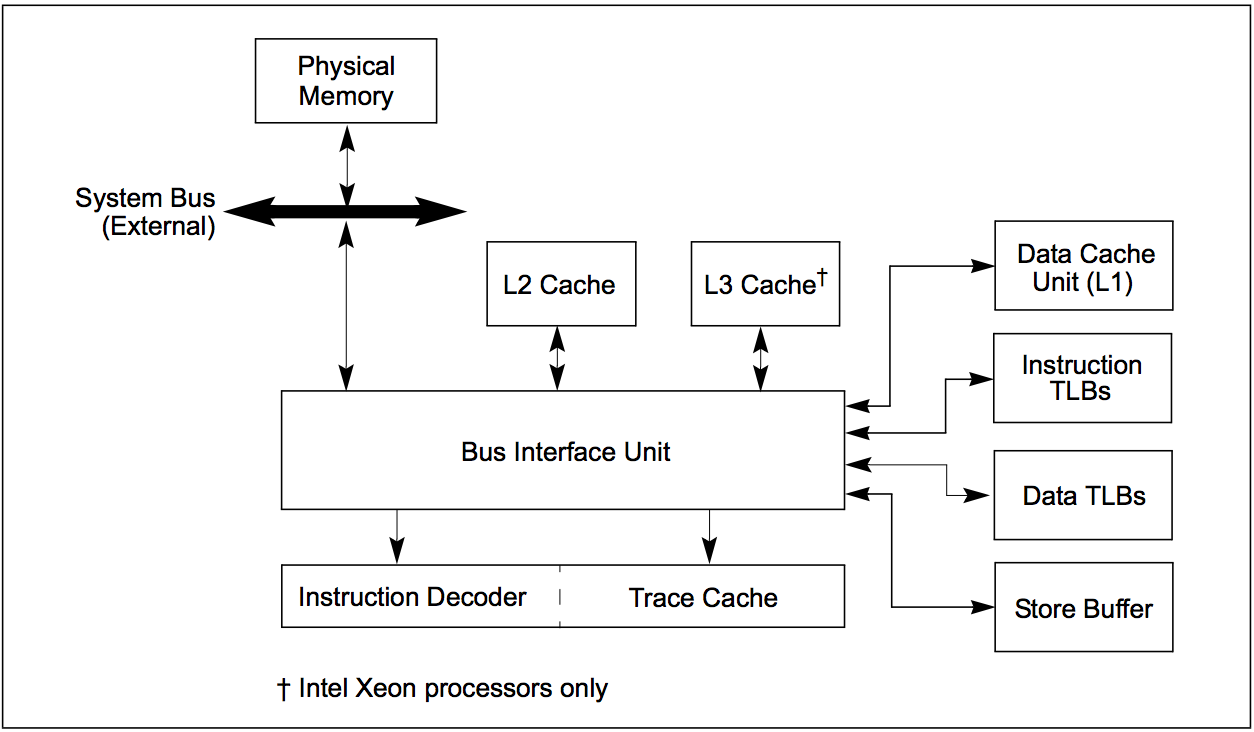
\includegraphics[width=145mm]{3/xeon_cache.png}
\caption{Cache Structure of the Pentium 4 and Intel Xeon Processors \cite{Intel2014}}
\label{xeon_cache_figure}
\end{figure}

Two other very important concepts are \textit{cache hits} and \textit{cache misses}. Cache hits occur when the cache can satisfy a request for the data required for further computation. If requested data cannot be found in the cache, of which the request was made, a cache miss occurs. Cache hits are a desired property of a computational system because they improve overall performance by reducing overhead caused by accessing data from bigger and slower levels of the memory hierarchy (e.g. RAM, a hard disk); system architects try to reduce the number of cache misses. Essentially, the larger the amount of data that can be provided directly from the cache, the greater the speed. The cache miss ratio is one of the ways to measure efficiency of cache usage; the lower the cache miss ratio, the faster the system is \cite{Chen2007}. Also, it is important to know that a \textit{cache line fill} happens when the CPU sees that a quantum of data, that is being read from memory, can be stored in a cache; the memory controller writes an entire cache line into the appropriate level(-s) of cache \cite{Intel2014}.

Studies indicate that fast cache-to-cache communication is crucial for achieving the best performance and scalability of multi-threaded programmes \cite{Molka2009,Lo2013,Zhang2010}. However, with increases in the clock rate, the system starts to suffer from the high level of cache miss ratio: caches are used more intensly. Heavy usage of processor hardware support (utilising larger caches and branch tables) and a bigger level of awareness on memory performance have helped processor designers manage cache misses and branches \cite{Jagtap2009}.

A term \textit{bus sniffing} is commonly used to describe a technique that is employed to support \textit{cache coherence}, i.e. the consistency of data stored in different levels of cache \cite{Hennessy2006}. Each controller of cache monitors instructions that may invalidate a cache line in the cache. They ensure that the same memory location is not loaded into more than one cache and if a quantum of data is requested, only one value is returned from all levels of memory \cite{Neupane2004}.

A fundamental decision in cache design is whether each piece of data can be stored in a cache once (in any cache line), or in only some of the lines \cite{Ostrovsky2010}. It is called \textit{cache associativity}. One may define three distinct types of cache associativity based on the way information is stored in the cache \cite{Hennessy2006}:

\begin{description}
  \item[Direct mapped cache] Each quantum of data can be saved in only a single cache line. It makes a cache block of data easy to find, but cache loses in flexibility of allocation of data.
  \item[N-way set associative cache] Every piece of data can be stored in one of N lines in the cache. For example, in a 8-way set associative cache, each quantum of data can saved in 8 different lines of cache. The index must be implemented to support locating data within the set.
  \item[Fully associative cache] Each quantum of information can be saved in any cache line; one may say that the cache works as a simple hash-table. Every tag associated with a quantum of data in the cache must be compared when looking for a block of data in the cache, but placement of data is simplified.
\end{description}

Figure \ref{cache_diagram} shows an example of a direct mapped cache and its interaction with blocks of data in main memory. Each block in main memory is associated with exactly one block in a cache.

\begin{figure}[ht!]
\centering
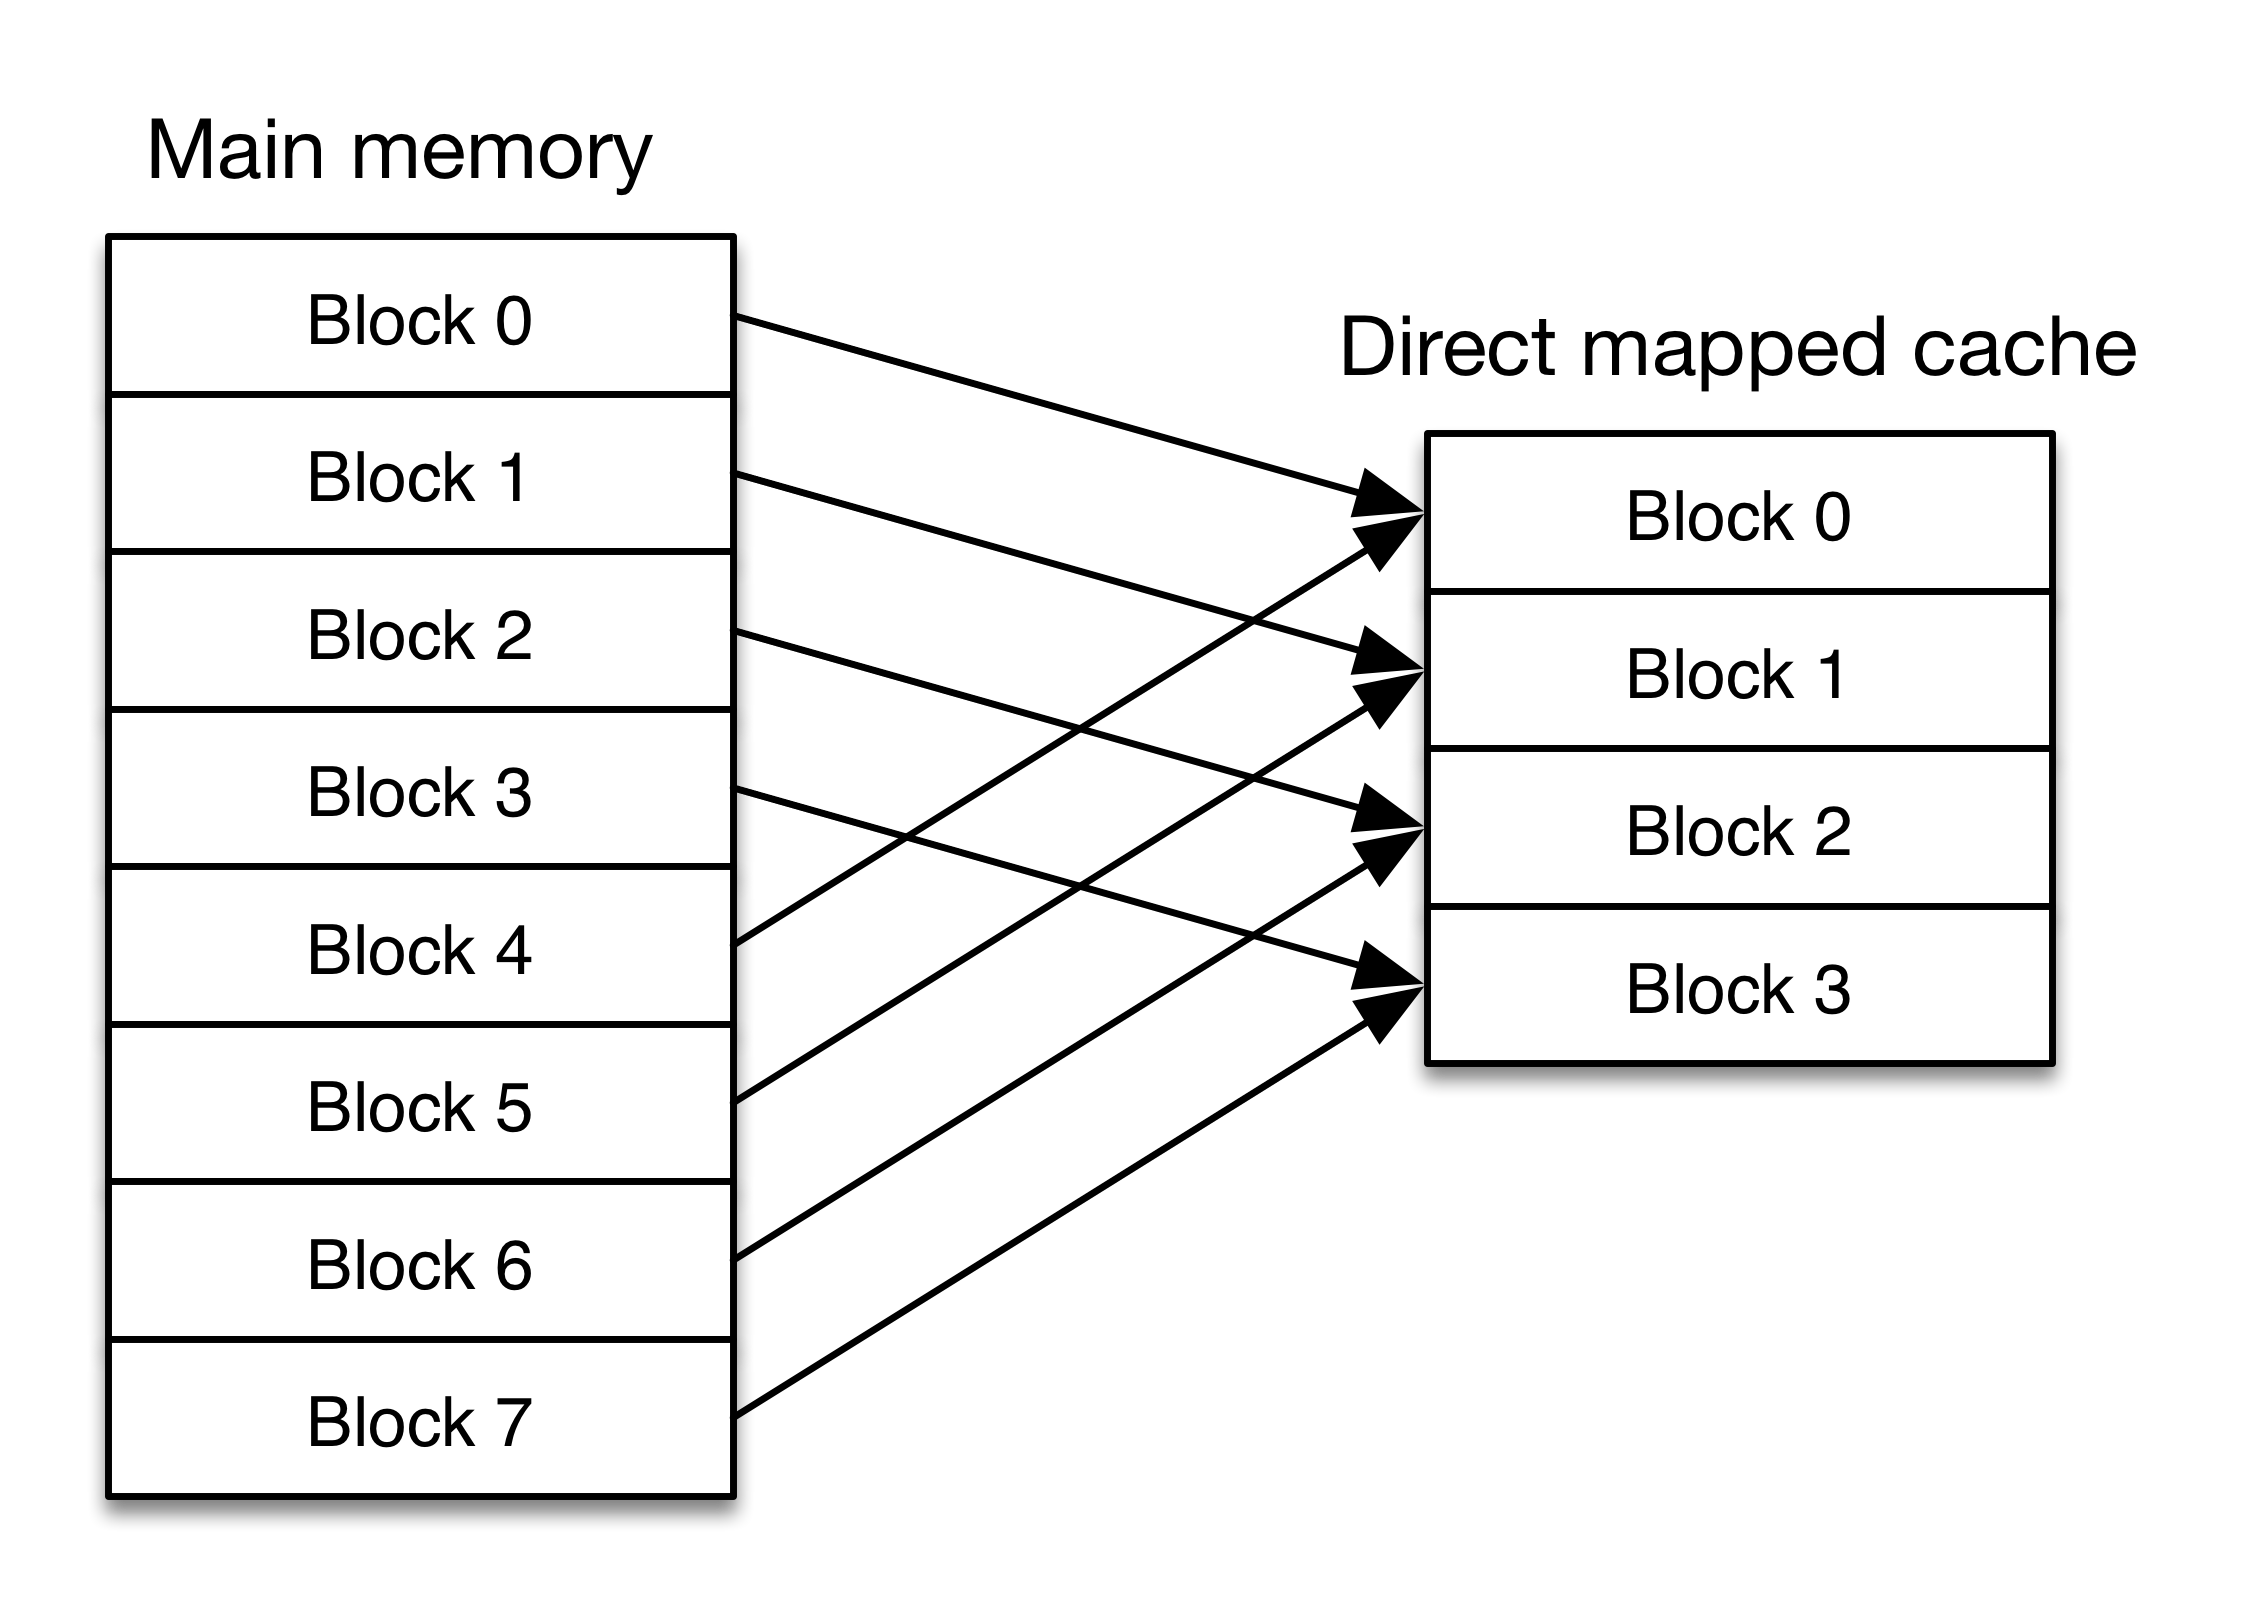
\includegraphics[width=100mm]{3/cache_diagram.png}
\caption{An example of a direct mapped cache}
\label{cache_diagram}
\end{figure}

Then, there are two main methods of caching (organising access to caches) available \cite{Intel2014}:

\begin{description}
  \item[Write-back (WB)] Both operations of writing and reading data to and from main memory are stored in caches. Data being cached is written only to the cache. The cached data is used to update main memory. This type of caching decreases bus traffic by eliminating many unnecessary writes to main memory. Processors used in this research have Write-back caches.
  \item[Write-through (WT)] Both operations of writing and reading data to and from main memory are also stored in caches. Data being cached is written both to the cache and to the main memory. When writing through to main memory, unused cache lines are not cleaned (indicate that it was unchanged since it was read from main memory), and valid cache lines are either filled (references memory in main memory when a word is not found in cache) or invalidated (marked as having incoherent copy of data in main memory). A write operation is not considered complete until the write to main memory is finished.
\end{description}

Finally, performance of processors is often impacted by implicit and explicit caching \cite{Intel2014}. \textit{Implicit caching} occurs when a piece of memory is marked as \textit{potentially cacheable}, although the element may never have been accessed. Implicit caching occurs in recent processor families due to data prefetching, branch prediction\footnote{\textit{Branch prediction}: when a CPU attempts to guess in which way a logical branch (e.g. if-then-else statement) will be executed before it can be known with certainty.}, and TLB miss handling. \textit{Explicit caching} is observed due to overuse of prefetch instructions (e.g. \textit{PREFETCHh} instruction, which was introduced in the Pentium III processor family). These instructions give ``hints" that a quantum of data will be used soon and should be cached as soon as possible. The explicit caching can lead to resource conflicts, which decrease the performance of an application. These events are difficult to handle on the software level and should be eliminated on the OS level.

\subsection{Cache Affinity}

One of the most commonly used metrics for measuring performance of multi-threaded systems is cache affinity \cite{Torrellas1995,Squillante1993,Vaswani1991}. Cache affinity is described as the amount of process's data or instructions stored inside of the cache. Affinity can be both high and low, depending on how much state has been accumulated. Speed of multi-threaded programmes is affected by the ability of processor cores to get access of required data by traveling through as few levels of cache and memory as possible \cite{Kazempour2008}. Cache affinity is often exploited by schedulers (algorithms that load-balance workload on processors) by rescheduling processes to run on a recently used processor.

Cache affinity has a direct impact on the level of cache misses in the system. The cache miss penalty to main memory, which costs hundreds of CPU cycles, and complexity of hardware that needs to be built, often reduce benefits that can be achieved from implementing instruction-level parallelism \cite{McKee2004}. Reduction of cache misses is beneficial for improving performance as well, as was shown in the project conducted by the author in the University of St Andrews \cite{Bazilinskyy2013}.

\subsection{Cache Latency and Throughput}

\textit{Cache latency} is the time taken to access a block of data in a cache. \textit{Cache throughput} is the amount of data that can be accessed in a unit of time. It is desirable to read as much data as quickly as possible, hence the lower the latency and the higher the throughput, the better.

CPUs often contain data \textit{prefetchers}, which transfer information into caches heuristically, i.e. they predict which data will also be accessed in the future and store it in the cache to be ready when required \cite{HasinaKhatoonShahidHafeezMirza2013}. By using the data prefetchers, one may reduce the amount of time that the CPU has to wait for the data to be fetched, i.e. data does not have to travel all the way from the main memory, but only from the faster cache. The Xeon processors used in the study utilise hardware data prefetchers \cite{Intel2009b}.

Applications often use data that is stored closely to what has been referenced recently, it is known as \textit{data locality}. There are two kinds of locality: 1) \textit{Temporal locality}: where there is a relatively big chance that a recently used quantum of data is likely to be used again in the near future; 2) \textit{Spatial locality}: pieces of data with nearby addresses are often referenced close together in time \cite{Denning2005}. Data Locality of information stored in the cache has a particularly large effect on the speed of multi-threaded applications \cite{ChenDing,Schneider2006}.

Data prefetchers use the principles of data locality and operate by analysing patterns in the access of data during the execution of programmes. Therefore, latency and throughput of accessing data depend on whether the prefetchers have been successful at comprehending the pattern of data usage and whether they have fetched the right piece of information into the caches. \cite[p.~811]{ward1990computation}

Cache latency and throughput affect both unichip and multichip systems. Benefits that can be received through reducing cache latency and increasing cache throughput differ across various multi-core architectures, i.e. multi-core uniprocessors and multi-core multiprocessors. The topic of the impact of the cache on speed of software has been discussed in the scientific community for more than two decades now; some examples of published results may be found in \cite{torrellas1995evaluating, Chen2007,VineethMekkatAnupHoleyPen-ChungYew2013}. The paper \cite{torrellas1995evaluating} proposed an algorithm for affinity-aware scheduling of threads that reduces the number of cache misses by up to 36\%; however, it was written in 1995 and the results cannot be considered as applicable to the modern-day computer architecture. The authors of \cite{Chen2007} merely discuss already built solutions that were developed in 1990s, and \cite{VineethMekkatAnupHoleyPen-ChungYew2013} focuses only on the shared last-level cache (LLC). Considerably fewer resources discuss the effect of cache on multi-core than on classic single-CPU architectures.

To summarize, the speed of multi-threaded programmes depends on a number of processes, as well as attributes associated with caches. This section has discussed a number of them: cache interference and cache miss ratio, the way caching is handled, and cache associativity. The context survey revealed that the impact of cache on data-sharing in multi-threaded environments is not covered extensively in published research. The motivation for this project came after realising that modern Linux kernels do not take the impact of the cache into account when scheduling of threads takes place in multi-core environments \cite{Bovet:2005:ULK:1077084,Aas2005}. Therefore, creation of a model of inter-thread communication in multi-core systems is investigated. The theoretical background offered by the model is tested by conducting a number of experiments on real hardware that form two distinct multi-core systems. A taxonomy of inter-thread communication is presented to support the model.

\section{Benchmarks for Testing Performance of Cache in Multi-Core Systems}
\label{sec:benchmarks}

A number of existing benchmarking suites were evaluated to understand if existing solutions could be utilised for answering the research questions. Providing a standardised set of tools for measuring and comparing performance of different parts of the system is currently a widely-discussed topic. Standardisation organisations\footnote{\url{http://www.spec.org/}} and conferences focused on the topic\footnote{\url{http://icpe2014.ipd.kit.edu/}}, that are meant to help software developers and hardware vendors, are emerging.

System- and component-level benchmarking tools were analysed. Namely: lmbench\footnote{\url{http://www.bitmover.com/lmbench/}}, Intel's VTune\footnote{\url{https://software.intel.com/en-us/intel-vtune-amplifier-xe}}, Valgrind\footnote{\url{http://valgrind.org/}}, and CPU2000\footnote{\url{https://www.spec.org/cpu2000/}}. VTune is a popular solution that is commonly used for fine-tuning high performance software that relies on hardware from Intel; it is not applicable to this study because of limited support for underlying libraries in the laboratory settings and lack of documentation on measuring latency and throughput of different layers of memory. It was found that Valgrind does not perform simulation on physical hardware, but, rather, through virtualisation, in this instance it cannot guarantee accuracy of results achieved from experiments. In addition, CPU2000 is an outdated product that is not supported by its developers and hence it offers little value to the scientific community. The tool lmbench is an open-source solution that was developed in early 1990s. Despite the lack of extensive documentation, it was possible to confirm that it is capable of checking latency of accessing cache.

% ---------------------------------------------------------------------------
%: ----------------------- end of thesis sub-document ------------------------
% ---------------------------------------------------------------------------


% this file is called up by thesis.tex
% content in this file will be fed into the main document

%: ----------------------- name of chapter  -------------------------
\chapter{Taxonomy and Model of Inter-Thread Communication} % top level followed by section, subsection
\label{chapterModel}

%: ----------------------- paths to graphics ------------------------

% change according to folder and file names
\ifpdf
    \graphicspath{{X/figures/PNG/}{X/figures/PDF/}{X/figures/}}
\else
    \graphicspath{{X/figures/EPS/}{X/figures/}}
\fi

%: ----------------------- contents from here ------------------------

This chapter describes a developed mathematical model of the involvement of cache in inter-thread data transfer. Creation of the exact model of what is expected when data is shared between threads that reside on different parts of the processor is a complex undertaking. Processor hardware is updated rapidly and each new generation of CPUs incorporates unseen before technologies that require more complex models that can describe the inter-thread communication. Such model is created to predict the impact of scheduling of the receiving thread for any CPU, it allows to generalise the proposed solution. It helps to develop the experiments that allow to characterise the performance of the data transfer through different levels of cache and main memory. In order to measure the impact of scheduling, the model is required as well. A number of resources of existing models of the cache are discussed in this chapter. Analysis of cache of inter-thread communication leads to a taxonomy shown in the next section. 

\section{Taxonomy of Inter-Thread Communication}
\label{taxonomy}

Multi-core systems handle usage of cache in multi-threaded programmes differently. Cache in most modern-day processors is organised in the following way: \textit{Level 1} (L1) and \textit{Level 2} (L2) data and instruction caches are private for each core and \textit{Level 3} (L3) cache is shared. Besides the mentioned in section \ref{cacheLit} Intel 64 architecture, such hierarchy is also commonly used in products of other manufacture, for example, IBM's POWER7 \cite{IBM2010} and AMD's Opteron \cite{Conway2011} chips that are utilised in servers and workstations. Additionally, in this type of architecture, private for each core levels of cache are inaccessible by private levels of cache associated with other cores. The private cores are each connected to the shared cache (normally L3) via the shared data bus. Providing external access to processors' cache memory is problematic, since caches from different levels have no direct physical connections between them. If one core needs to access data that is stored in another core's cache, the only way to receive required information is through the system bus.

In case of a processor where each core has a private L1 cache and shared between cores of the same CPU L2 caches, there can be three main patterns of thread communication. Refer to Figure \ref{Threads_cpu_diagram} for a diagram that outlines these patterns. It is assumed that no thread scheduling takes place. 

\begin{figure}[ht!]
\centering
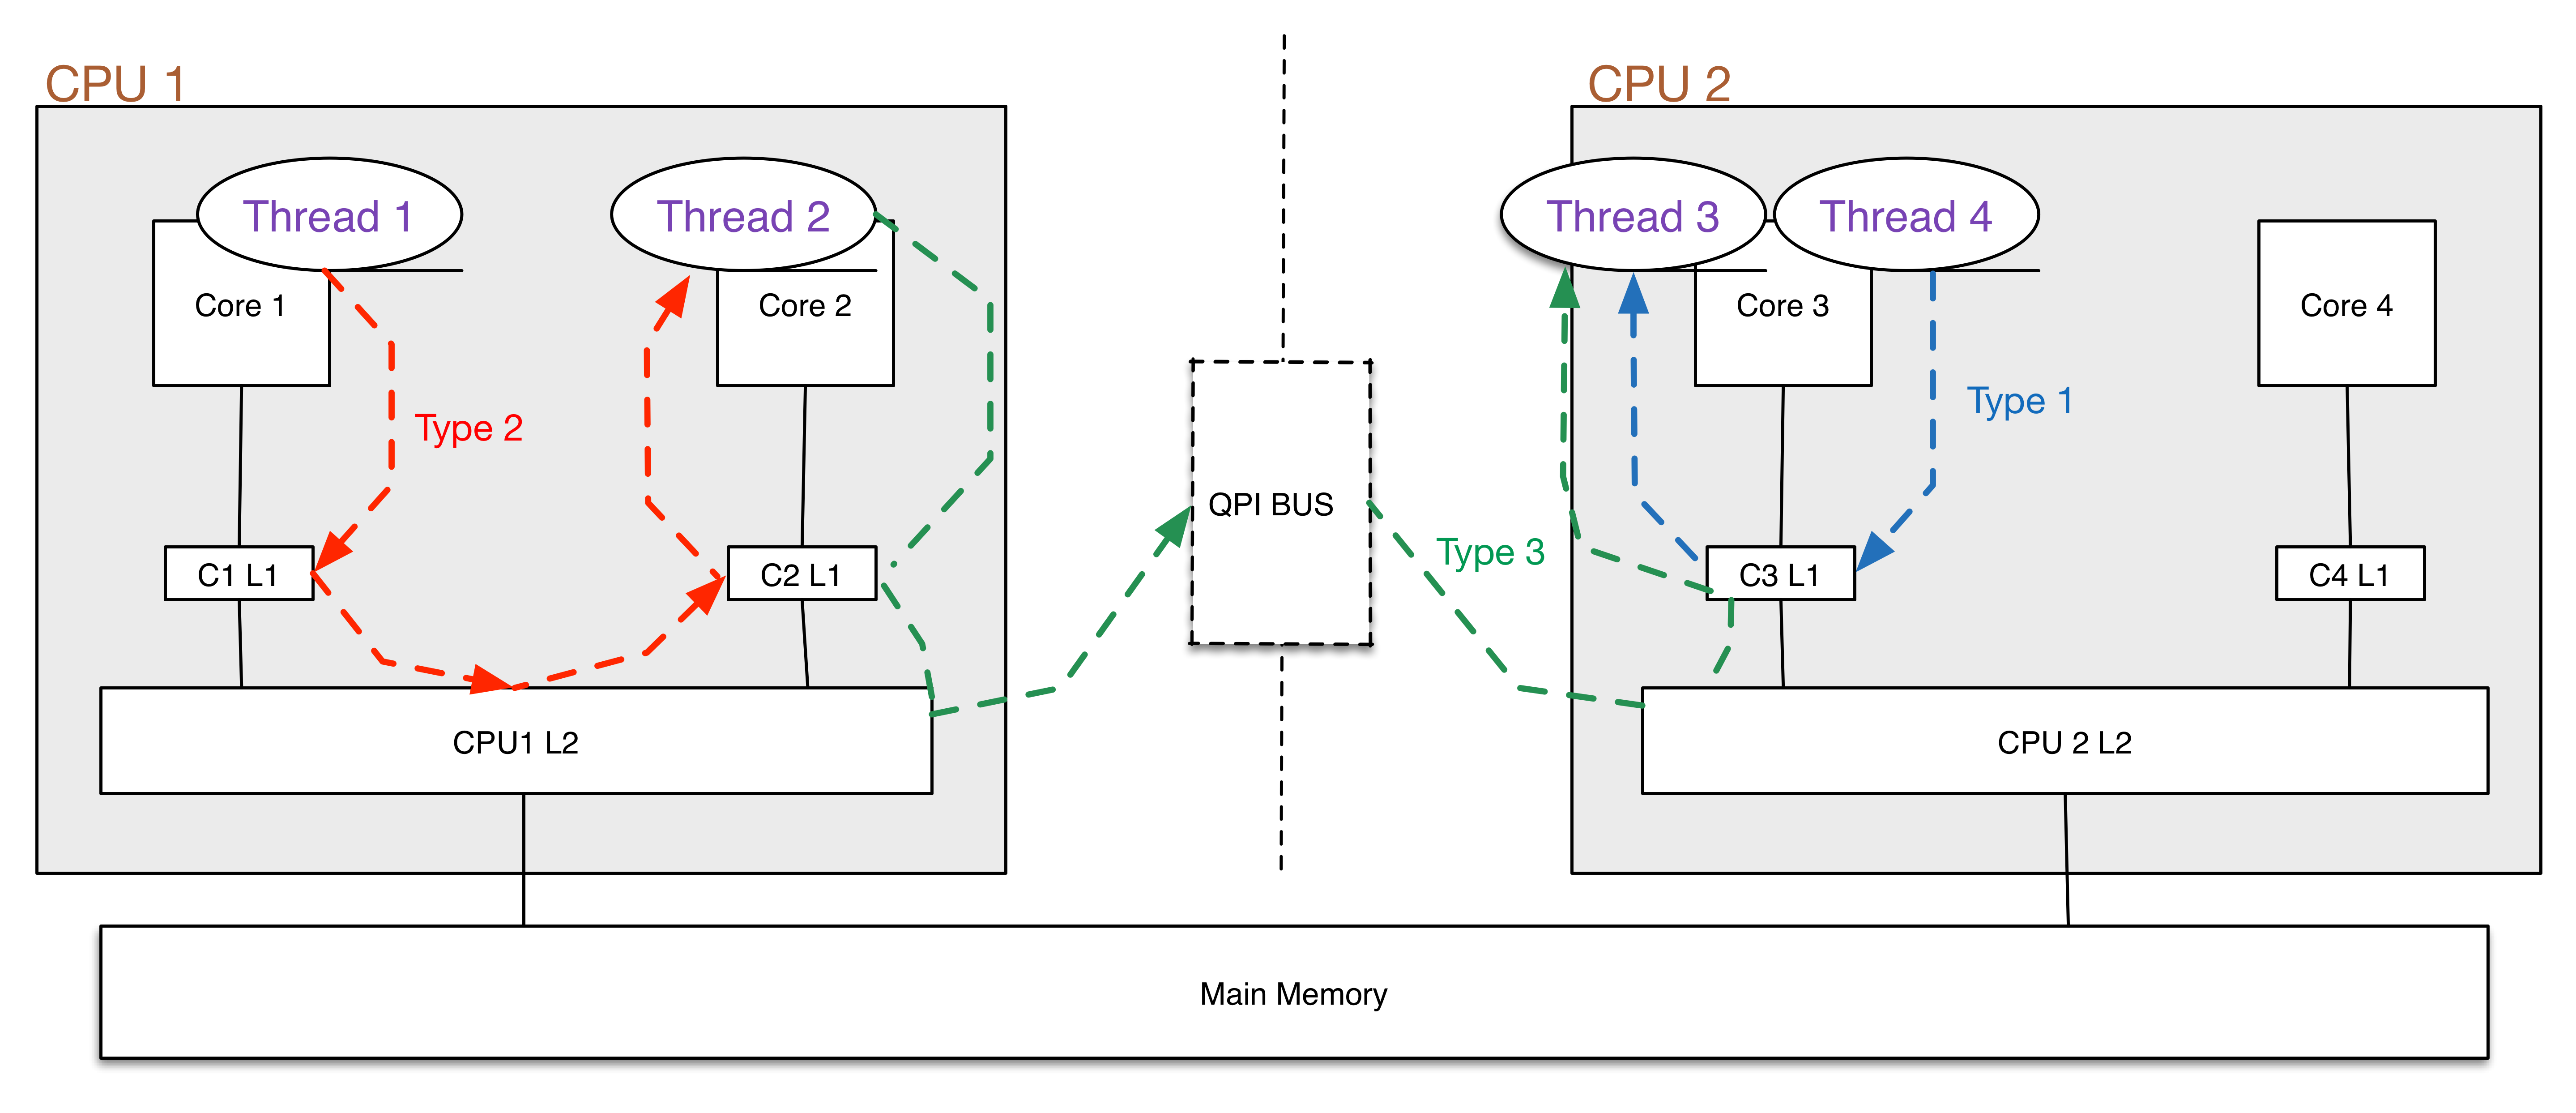
\includegraphics[width=145mm]{3/Threads_cpu_diagram.png}
\caption{Communication between threads in a multi-core environment}
\label{Threads_cpu_diagram}
\end{figure}

The following list presents the taxonomy of inter-thread exchange of data that defines three types of communication:

\begin{description}
  \item[Type 1] The simplest case that is associated with the least amount of overhead caused by moving data between threads (Thread 3 and Thread 4) is communication between two threads that reside on \textit{the same CPU, same core}. The blue line on the figure represents this scenario.
  \item[Type 2] Communication takes place between two threads that are executed by \textit{the same CPU, but they reside on different cores}; this type of communication is more expensive\footnote{\textit{expensive} -- takes a significant amount of time to execute.} computation-wise (compared to Type 1) because different L1 and L2 caches are utilised when the threads use shared data. The red line on the diagram shows an example of communication of this type. 
  \item[Type 3] The most complicated case involves all three levels of cache. In this case data is shared between threads that reside \textit{on different chips}. An inter-chip bus has to be used. The green line points to an example of communication of this type
\end{description}

The cost of inter-thread communication depends on the nature of the task that needs to be performed (i.e. amount of I/O, amount of data used etc.), the environment (primarily the choice of the processor) and a number of other attributes of the system used. Usage of a scheduler that is cache-aware may greatly improve the efficiency of cache in multi-core systems and hence the overall performance. One may find a few schedulers that are aimed at multi-threaded programmes \cite{Zhuravlev2012,Liaskovitis2006,Chen2007}. Two systems that claim to support cache-aware scheduling are Parallels Depth First (PDF)\cite{Blelloch1999} and Work Stealing (WS)\cite{Blumofe1994}. Both of them were built in 1990s, in the pre-multichip era.

\section{Model of Inter-Thread Communication}
\label{modelsection}

A number of resources discuss existing models of the cache \cite{ChenDing,Agarwal1989,Song2007}. A model suggested by the authors of \cite{ChenDing} was thoughtfully tested by a number of benchmarks and the findings presented in the paper were used as motivation for creation of the proposed in this section model. However, the referred model does not take into account exchange of data on the main memory level. Similarly, \cite{Song2007} discusses the L2 cache only. Work published in \cite{Agarwal1989} was conducted in the end of 1980s, and the proposed in that paper model proves to be too abstract, when applied to current computer architectures. A few papers discuss the implications of conducting simulations \cite{Heidelberger1990,Archibald1986,Zhao2011} rather than describing the behaviour of cache by means of mathematical modelling. The mathematical description of the inter-thread communication provides a much more solid grounding for further research. Creation of such model is undertaken within the scope of this study, because it allows to predict the impact of scheduling decisions for any CPU that the model can be applied for.

The proposed model describes communication between two threads that reside on a system that has three levels of cache. The Level 1 caches are private for each core, the Level 2 caches are private for each chip. The Level 3 caches are private for each chip, but, in case of most modern-day processors, they are connected by a bus, which, effectively, unites them and combines the caches into one shared across the whole processor entity. Such model is later tested by performing experiments on the real hardware.

The activity being analysed in this model is where the first thread Th1 writes data into caches, making the thread the sending end, and the second thread Th2 reads data, which makes it the receiving end. Time, which needs to be spent on writing data to a buffer in one thread, and then reading it out of that buffer in another thread, is modelled. The interaction between the size of the buffer and the cache size(s) is modelled. This scenario is an example of a simplified version of a typical ``client--server" application. Such programmes can often be seen in the telecommunication industry, where large quantities of data are exchanged between clients and servers. Analysis of such simplified case can be a base for further work that involves more complicated programmes.

There is one variable in the model: the size of data that is shared between two threads $n$. The quantum of stored data is one cache line (typically 64 or 128 bytes). Depending on the size of used data, information is stored in a cache (-s) of a particular level; i.e. if data fits into Level 1 cache, it is stored there, if not, it is cached in the next level of cache -- Level 2 cache.

The latency of using shared between two threads data (Thread 1 writes data into a cache or main memory and Thread 2 reads data from the cache or main memory) $d_{comm}$ can be described by an equation \eqref{eq:model1}:

\begin{equation}\label{eq:model1}
d_{comm} = d_{write} + Control + d_{read}
\end{equation}

, where the cost of writing data into the cache $d_{write}$ is described by equation \eqref{eq:model2}:

\begin{equation}\label{eq:model2}
d_{write} = \begin{cases}d_{WriteL1}= n/ns * lat_{WriteL1} & n \leq l_{L1}\\d_{WriteL2} = n/cls * lat_{WriteL2} + l1w & l_{L1} < n \leq l_{L2}\\d_{WriteL3} = n/cls * lat_{WriteMem} + l1w & l_{L2} < n \leq l_{L3}\\d_{WriteMem} = n/cls * lat_{WriteMem} + l1w & n > l_{L3}\end{cases}
\end{equation}

, where $l_{L1}$, $l_{L2}$, $l_{L3}$ indicate sizes of Level 1, Level 2, and Level 3 caches respectively. $ns$ points to the size of one word of data that is written in cache, e.g. 4 bytes for a case of using \textit{long} on most systems. As described in section \ref{cacheLit}, the minimum amount of data that can be fetched from caches is a cache line; in this model, $cls$ is the size of one cache line. $l1w$ indicates the cost of writing the amount of memory that can fit into Level 1 cache. In most cases this number is small and can be neglected. The model assumes that direct mapped caches are used.

\begin{equation}\label{eq:model20}
l1w = (n/ns - n/cls) *  lat_{WriteL1}
\end{equation}

Figure \ref{cacheline} gives an example of writing and reading one cache line, when the access is initiated from main memory. In this case the size of a cache line is 64 bytes and long words (4 bytes each) are written/read. The first write/read is very expensive because all levels of memory are used and its latency is equal to the latency of the level in memory, from which the operation was initiated. All subsequent actions are performed solemnly on the Level 1 cache and the latency of such operations equals to the latency of Level 1 cache. $l1w$ can be expressed by equation \ref{eq:model20}. The caches are assumed to be fully associative for simplicity, i.e. n-associativity of cache is ignored. It is also assumed that neither pipelining no simultaneous execution of multiple instructions are implemented.

\begin{figure}[ht!]
\centering
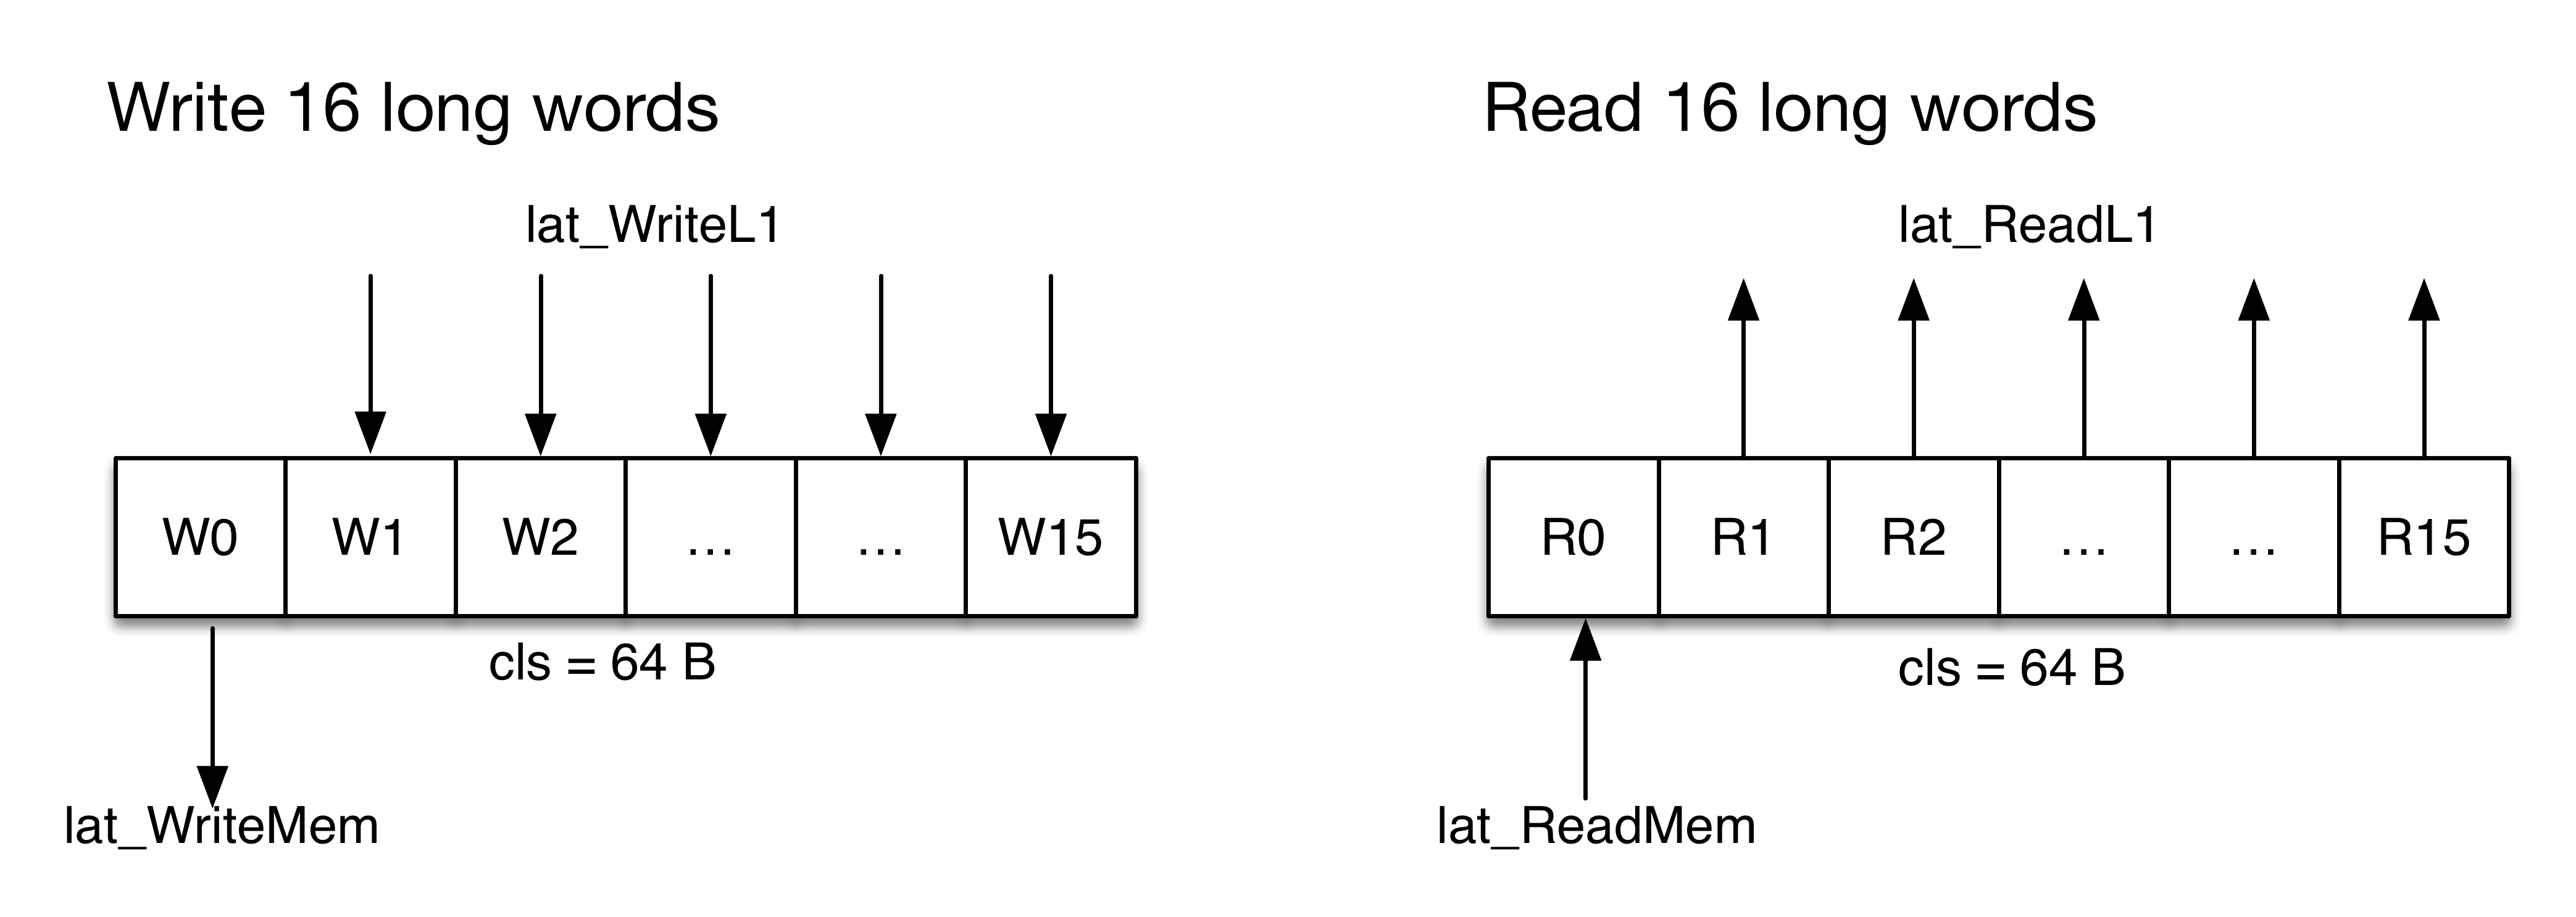
\includegraphics[width=145mm]{3/cacheline.png}
\caption{Writing and reading a cache line in a Write-back cache}
\label{cacheline}
\end{figure}

Utilisation of threads implies that there will also be overhead caused by the control element. In the situation of having two POSIX-threads\footnote{\textit{POSIX-threds} is a POSIX standard for threads. This technology is utilised to control threads in a multi-threaded environment in the project.} working with shared data, the overhead is caused by stopping the 1$^{\textnormal{st}}$ thread, yielding the CPU, scheduling and starting the 2$^{\textnormal{nd}}$ thread that starts to use shared data that is implanted into the cache/main memory by the 1$^{\textnormal{st}}$ thread. This overhead does not depend on the variable, which is the size of data shared between the threads. Such overhead $Control$ is described in equation \eqref{eq:model3}. This equation also defined the non-deterministic part of the equation $I$, which indicates the overhead caused by the unwanted events: $I_{int}$ -- interrupts, $I_{cs}$ -- context switches, $I_{pf\_maj}$ -- major page fault, and $I_{pf\_min}$ -- minor page faults. As discussed in section \ref{OSinterference}, context switches and interrupts always occur together and their impact can be united into a single parameter $I_{ics}$.

\begin{equation}\label{eq:model3}
\begin{split}
Control = Control_{exitTh1} + Control_{tt} + Control_{enterTh2} + I \\
I = I_{int} + I_{cs} + I_{pf\_maj} + I_{pf\_min} \\
I_{ics} = I_{int} + I_{cs} \\
Control = Control_{exitTh1} + Control_{tt} + Control_{enterTh2} + I_{ics} + I_{pf\_maj} + I_{pf\_min} \\
\end{split}
\end{equation}

, where $Control_{exitTh1}$ indicates the amount of time the Operating System needs to spend to exit Thread 1, $Control_{tt}$ expresses the amount of time required to switch between threads and $Control_{enterTh2}$ shows how much time the OS has to spend on giving control to the 2$^{\textnormal{nd}}$ thread that needs to copy data from the shared memory. The amount of overhead represented by $Control_{exitTh1}$, $Control_{tt}$, and $Control_{enterTh2}$ represents a determenistic parameter that can be measured once. The proposed model is applicable to all three types of inter-thread communication as described in the taxonomy in section \ref{taxonomy}. Finally, the cost of reading data from the cache or main memory $d_{read}$ is described by equation \eqref{eq:model4}:

\begin{equation}\label{eq:model4}
d_{read} = \begin{cases}d_{ReadL1}= n/ns * lat_{ReadL1} & n \leq l_{L1}\\d_{ReadL2} = n/cls * lat_{ReadL2} + l1r & l_{L1} < n \leq l_{L2}\\d_{ReadL3} = n/cls * lat_{ReadL3} + l1r & l_{L2} < n \leq l_{L3}\\d_{ReadMem} = n/cls * lat_{ReadMem} + l1r & n > l_{L3}\end{cases}
\end{equation}

, where, similarly to the equation \ref{eq:model2}, $l_{L1}$, $l_{L2}$, $l_{L3}$ indicate the amounts of data that can fit in Level 1, Level 2, and Level 3 caches respectively.

Latencies of writing data into different levels of cache $lat_{WriteL1}$, $lat_{WriteL2}$, $lat_{WriteL3}$ and main memory $lat_{WriteMem}$ are constants. Similarly, latencies of reading data from different levels of cache $lat_{ReadL1}$, $lat_{ReadL2}$, $lat_{ReadL3}$ and main memory $lat_{ReadMem}$ are also constants. $l1r$ indicates the cost of reading the amount of memory that can fit into Level 1 cache. This model assumes that a Write-back cache is used. In the scope of this research we assume that:

\begin{equation}\label{eq:model5}
\begin{split}
lat_{WriteL1} = lat_{ReadL1} \\
lat_{WriteL2} = lat_{ReadL2} \\
lat_{WriteL3} = lat_{ReadL3} \\
lat_{WriteMem} = lat_{ReadMem} \\
l1r = l1w \\
\end{split}
\end{equation}

Finally, the latency of using data exchanged between two threads may be described by the following equation \ref{eq:model10}:

\begin{equation}\label{eq:model10}
\begin{split}
d_{comm} = \begin{cases}d_{WriteL1}= n/ns * lat_{WriteL1} & n \leq l_{L1}\\d_{WriteL2} = n/cls * lat_{WriteL2} + l1w & l_{L1} < n \leq l_{L2}\\d_{WriteL3} = n/cls * lat_{WriteMem} + l1w & l_{L2} < n \leq l_{L3}\\d_{WriteMem} = n/cls * lat_{WriteMem} + l1w & n > l_{L3}\end{cases} \\ + Control_{exitTh1} + Control_{tt} + Control_{enterTh2} + I_{ics} + I_{pf\_maj} + I_{pf\_min} \\ + \begin{cases}d_{ReadL1}= n * lat_{ReadL1} & n \leq l_{L1}\\d_{ReadL2} = n/cls * lat_{ReadL2} + l1r & l_{L1} < n \leq l_{L2}\\d_{ReadL3} = n/cls * lat_{ReadMem} + l1r & l_{L2} < n \leq l_{L3}\\d_{ReadMem} = n/cls * lat_{ReadMem} + l1r & n > l_{L3}\end{cases}
\end{split}
\end{equation}

The parameters in the model are determined through experimentation (as the CPU specification does not include this level of detail). The cycle-level experiments are described in section \ref{design_cycle_level}. Data received from the experiments help quantify the model. Three application-level experiments were engineered to measure the impact of the cache in two real-life settings and verify the proposed model. Also, an additional experiment was developed; it measures how much time interrupts and minor page faults take, it is aimed to receive values for $I_{ics}$ and $I_{pf\_min}$. Refer to section \ref{app_design} for the description of the experiments. Results from the application-level experiments are used to verify the model and investigate the ways of improving its accuracy. Chapter \ref{discussionChapter} discusses findings received after executing the experiments and their applicability to the model and this study in general.
% ---------------------------------------------------------------------------
%: ----------------------- end of thesis sub-document ------------------------
% ---------------------------------------------------------------------------


% this file is called up by thesis.tex
% content in this file will be fed into the main document

%: ----------------------- name of chapter  -------------------------
\chapter{Experimental Environment and Experiments} % top level followed by section, subsection


%: ----------------------- paths to graphics ------------------------

% change according to folder and file names
\ifpdf
    \graphicspath{{X/figures/PNG/}{X/figures/PDF/}{X/figures/}}
\else
    \graphicspath{{X/figures/EPS/}{X/figures/}}
\fi

%: ----------------------- contents from here ------------------------


This chapter introduces the experimental environment and how the environment was designed and developed to receive results, which do not include overhead from the Operating System and support time measurements with nano-second accuracy. The chapter also describes the experiments that are used in the practical part of this project. The experiments were developed because described in section \ref{sec:benchmarks} benchmarking tools cannot provide precise and trustworthy information to parametrise the model. Both this chapter and chapter \ref{chapterCondExp} contain a great number of details; it should allow a reader to replicate the study, if required.

Figure \ref{exp_env_exp} outlines the structure of the proposed solution. This part of the document starts from describing the file structure, which lies in the base of all elements of the solution. The experimental environment is used to set-up the laboratory setting that is capable of monitoring unwanted events imposed by the OS and provide accurate time measurements with nano-second level of accuracy. A number of cycle- and application-level experiments are executed from the experimental environment. Gathered from running experiments data is recorded into CSV files / outputted on the screen by the experimental environment.

\begin{figure}[ht!]
\centering
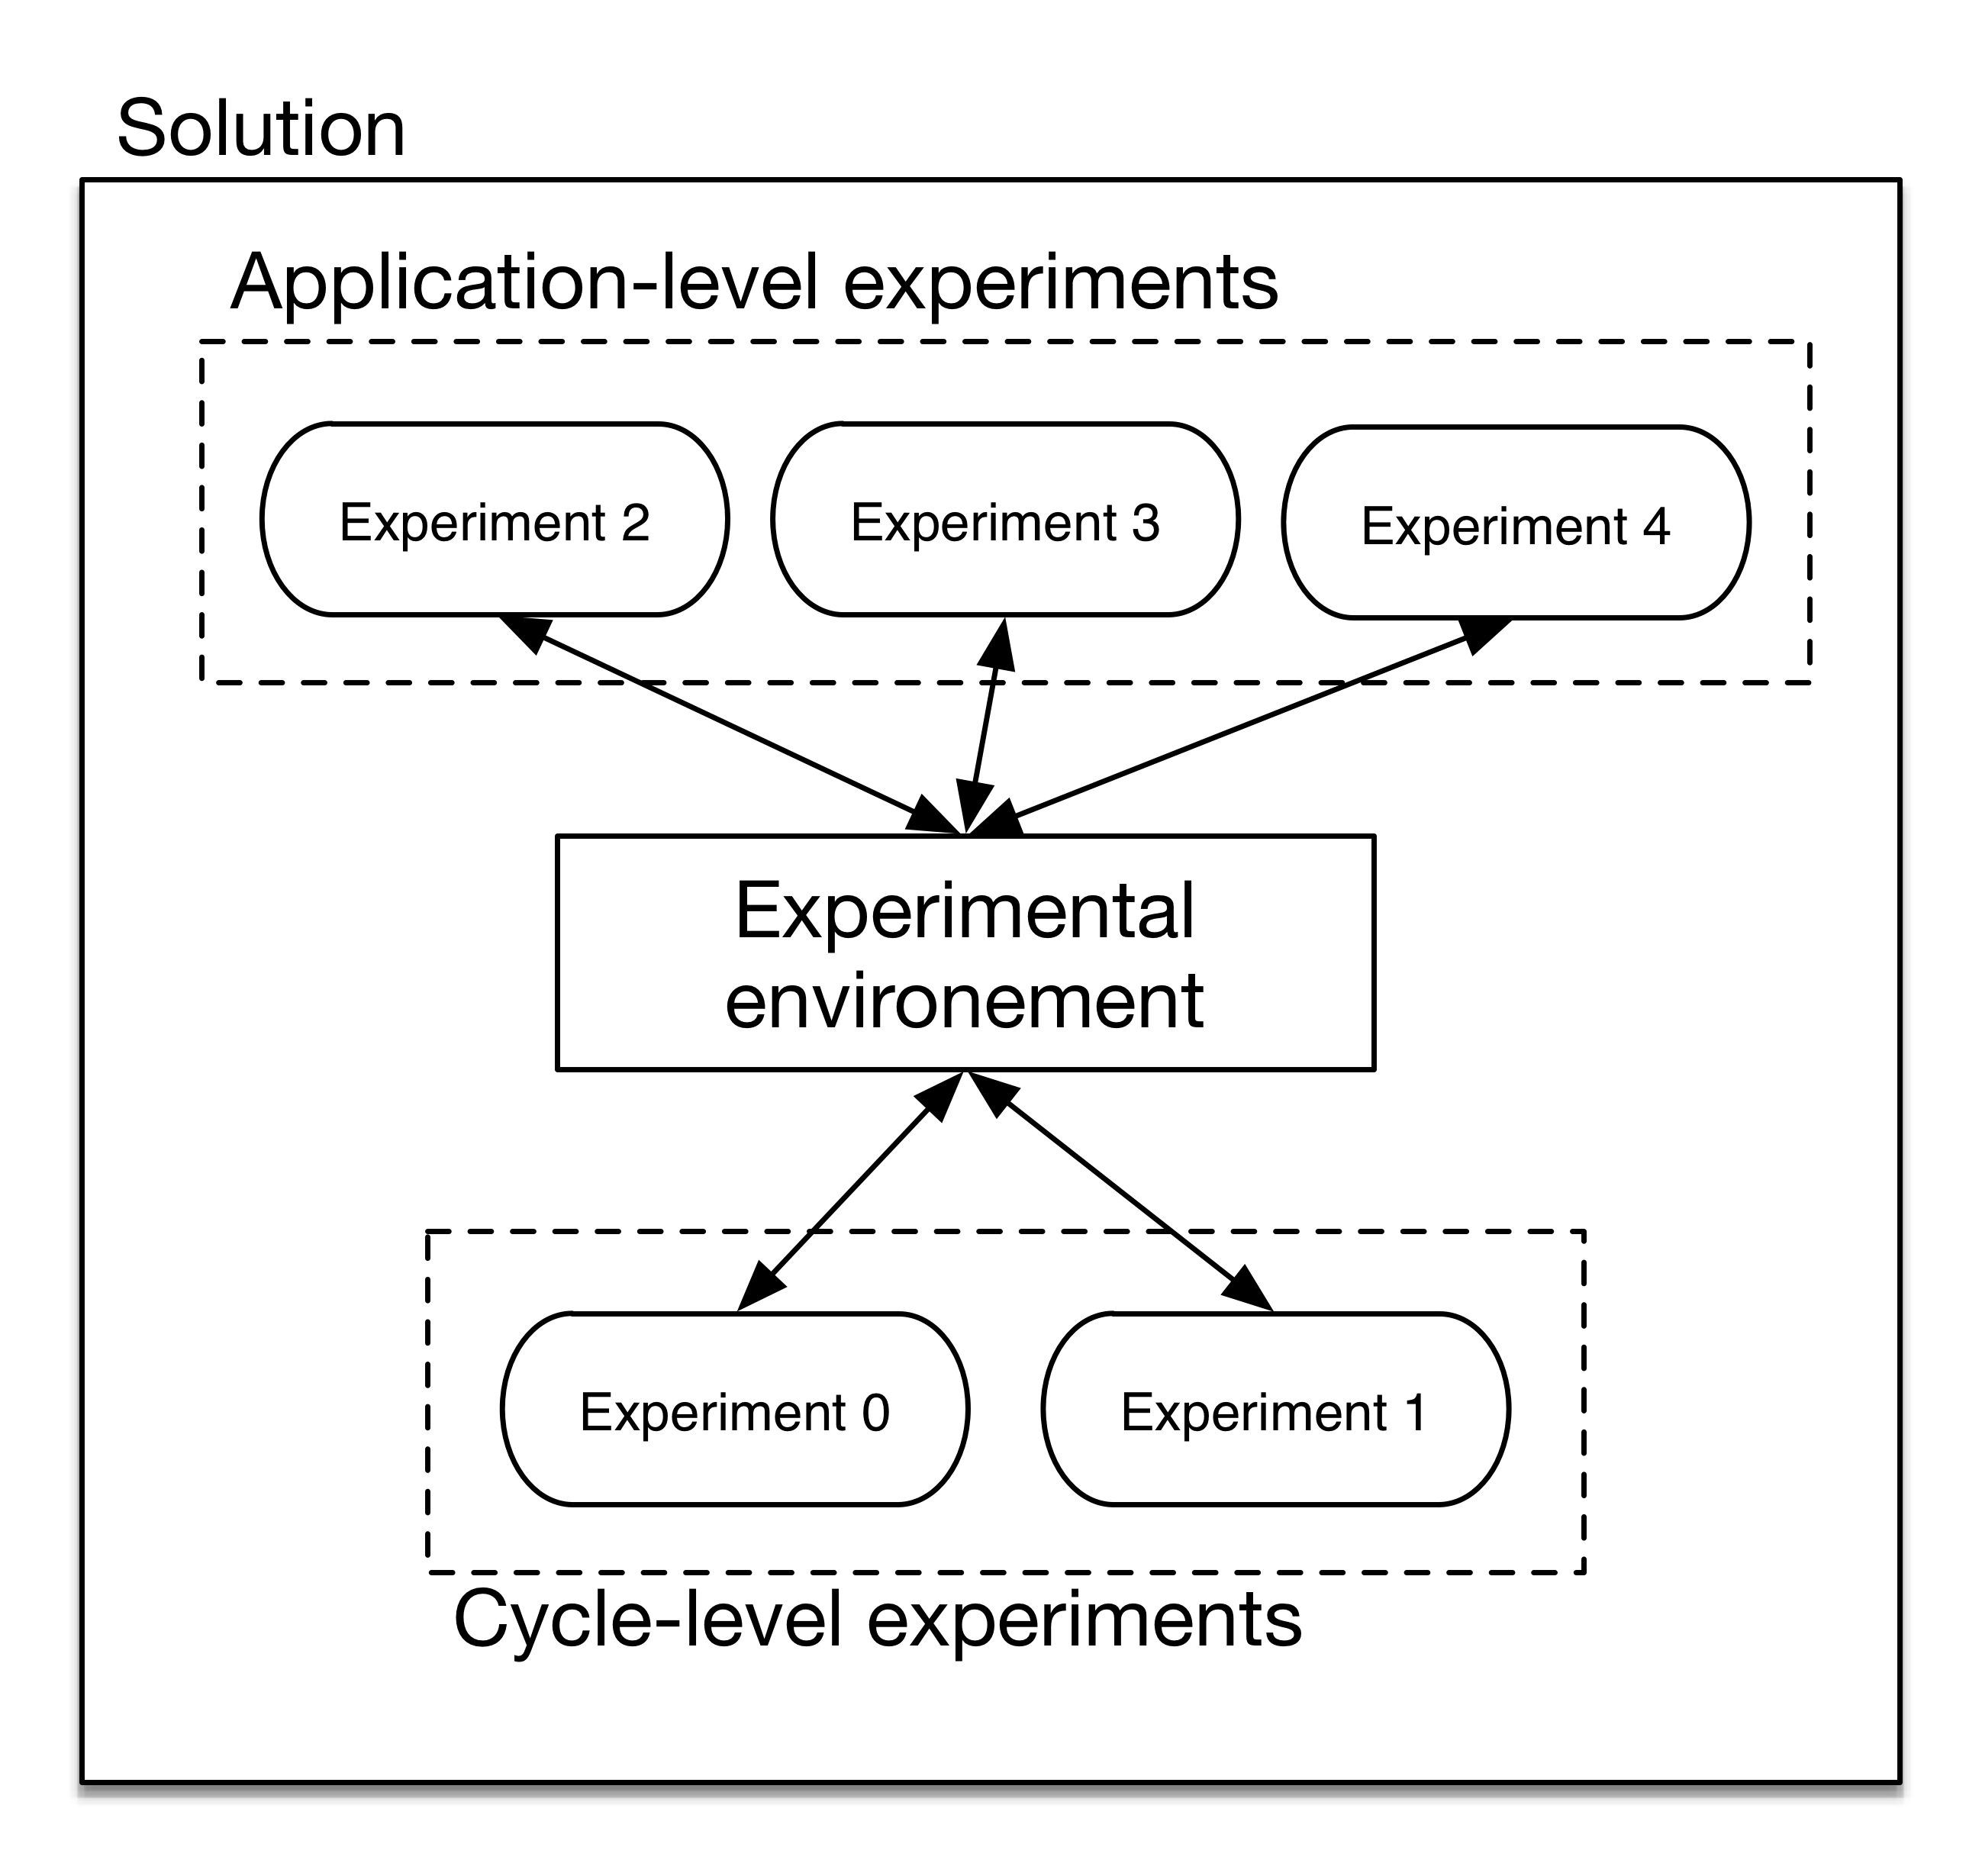
\includegraphics[width=90mm]{4/exp_env_exp.png}
\caption{Overview of the solution}
\label{exp_env_exp}
\end{figure}

Refer to the flowchart \ref{flowExperiment}, it outlines the actions that take place when experiments are run. The sections of this chapter give a detailed description of all processes that are present on the figure.

\begin{figure}[ht!]
\centering
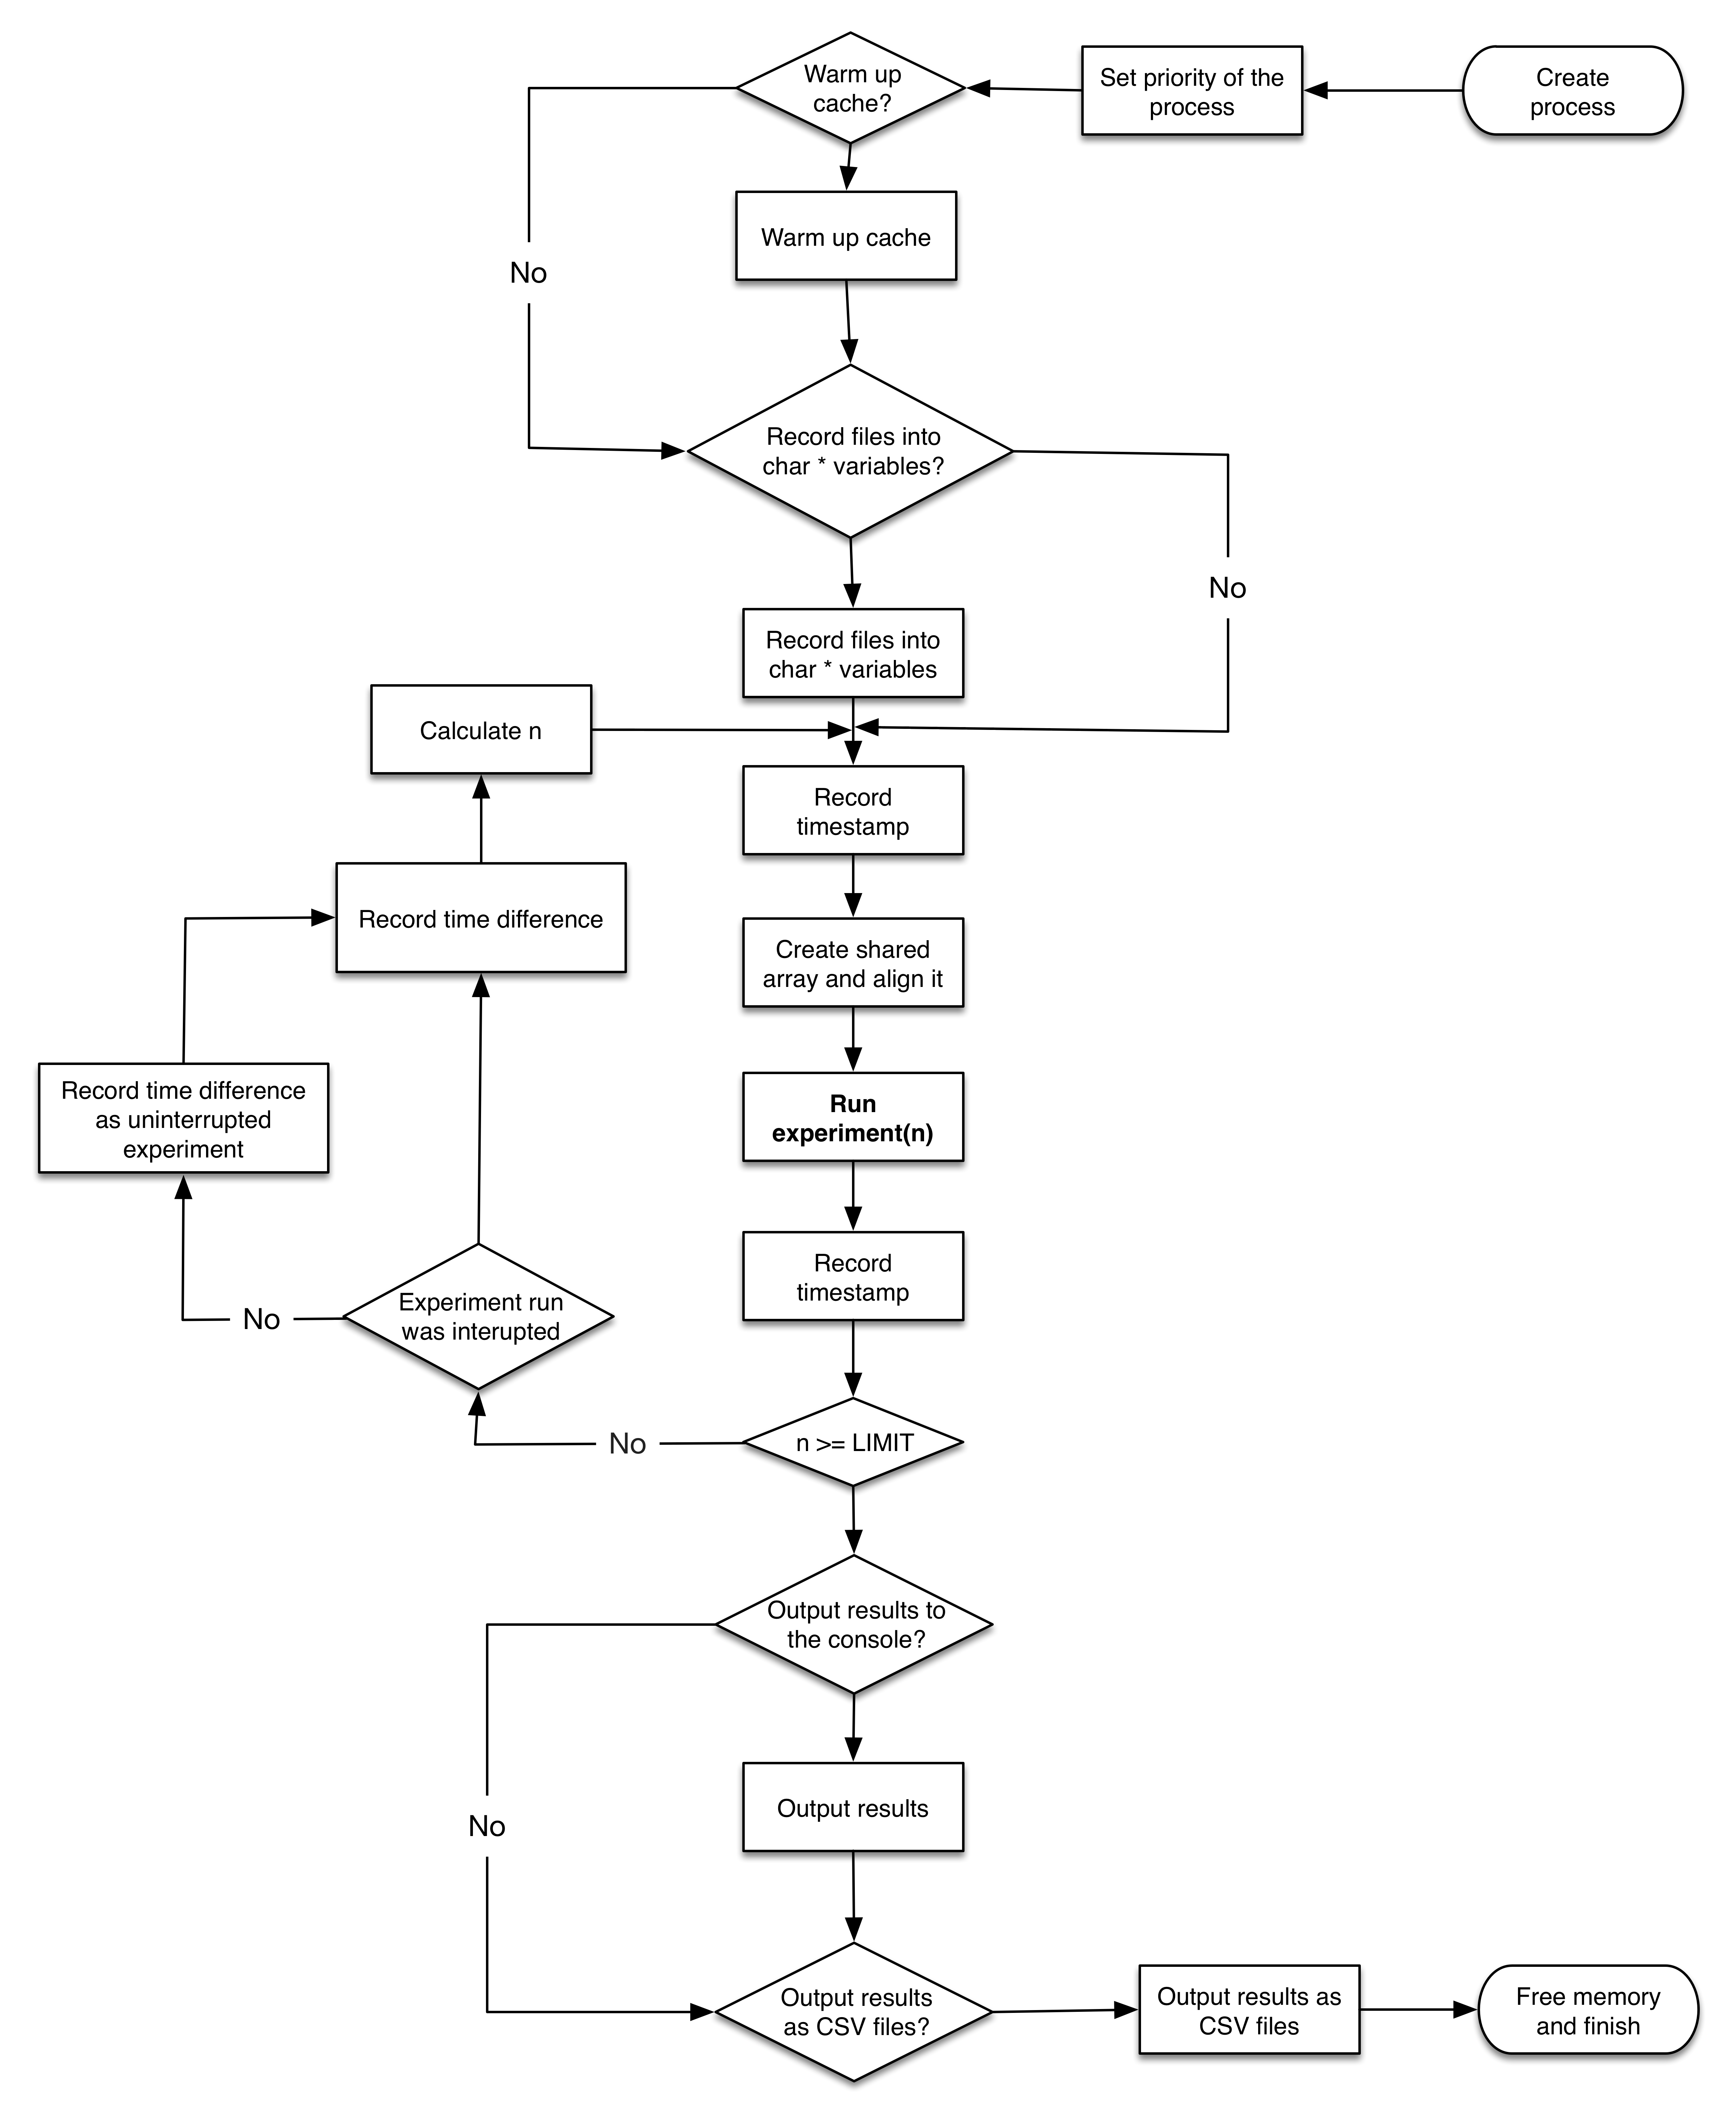
\includegraphics[width=145mm]{4/flow_experiment.png}
\caption{A diagram showing the flow of the process of running an experiment}
\label{flowExperiment}
\end{figure}

The rest of the chapter describes the proposed solution in details.

\section{Organisation of Solution}
\label{fileStrcture}

Even though the structure of the solution is a low-level detail, it is presented in the beginning of the chapter since specific files are referenced throughout the chapter. The C language was used because it has support of working with hardware and kernels of Operating Systems (e.g. by means of the Assembly language), as well as the fact that C does not impose high-level programming structures, such as tools that facilitate the object oriented programming paradigm (like in C++). Additionally, the hardware that was chosen for running experiments is capable of compiling and running programmes written in C without any additional configuration.

All files with the solution described in this section may be found in a folder \textit{``src"}\footnote{\url{https://github.com/Hollgam/cache-mt/tree/master/src/}}. Additional testing programmes are located in other folders, which are referenced when the programmes are discussed. The main files are listed below:

\begin{description}
  \item[clock\_gettime\_mac.c] The implementation of \textit{clock\_gettime(3)} for Mac OS.\footnote{\url{https://github.com/Hollgam/cache-mt/tree/master/src/clock\_gettime\_mac.c}}
  \item[clock\_gettime\_mac.h] The header file for the implementation of \textit{clock\_gettime(3)} for Mac OS.\footnote{\url{https://github.com/Hollgam/cache-mt/tree/master/src/clock\_gettime\_mac.h}}
  \item[conf.h] The configuration file. A number of constants that alter behaviour of the experimental environment are defined in the file.\footnote{\url{https://github.com/Hollgam/cache-mt/tree/master/src/conf.h}}
  \item[experiments.c] The implementation of the experiments.\footnote{\url{https://github.com/Hollgam/cache-mt/tree/master/src/experiments.c}}
  \item[experiments.h] The header for the implementation of the experiments.\footnote{\url{https://github.com/Hollgam/cache-mt/tree/master/src/experiments.h}}
  \item[file\_worker.c] The implementation of a number of functions that support file I/O.\footnote{\url{https://github.com/Hollgam/cache-mt/tree/master/src/file\_worker.c}}
  \item[file\_worker.h] The header for the implementation of a number of functions that support file I/O.\footnote{\url{https://github.com/Hollgam/cache-mt/tree/master/src/file\_worker.h}}
  \item[hr\_timer.c] The cross-platform high-resolution timer for performance measurements.\footnote{\url{https://github.com/Hollgam/cache-mt/tree/master/src/hr\_worker.c}}
  \item[hr\_timer.h] The header for the cross-platform high-resolution timer for performance measurements.\footnote{\url{https://github.com/Hollgam/cache-mt/tree/master/src/file\_worker.h}}
  \item[makefile] Makefile\footnote{\textit{Makefile} is a description file used by the make utility that creates executable files based on the source code and libraries.} for the project.\footnote{\url{https://github.com/Hollgam/cache-mt/tree/master/src/makefile}}
  \item[test\_env.c] A number of functions that support the experimental environment.\footnote{\url{https://github.com/Hollgam/cache-mt/tree/master/src/test\_env.c}}
  \item[test\_env.h] The header for the experimental environment.\footnote{\url{https://github.com/Hollgam/cache-mt/tree/master/src/test\_env.h}}
  \item[test.c] The main entry point of the programme. It prepares the experimental environment and executes the experiments.\footnote{\url{https://github.com/Hollgam/cache-mt/tree/master/src/test.c}}
  \item[test.h] The header for the main entry point.\footnote{\url{https://github.com/Hollgam/cache-mt/tree/master/src/test.h}}
\end{description}

Additional programmes written to test various aspects of the work of CPUs that are mentioned throughout this chapter may be found in other directories: \textit{test\_clockgettime}, \textit{test\_pagefault\_fopen}, \textit{test\_rdtsc}, and \textit{test\_time\_interrupt}.

\section{Experiments}
\label{experimentsDesign}

Two cycle- and three application-level experiments were designed to receive data on latency of different levels of cache, provide a framework to verify the model, and estimate an impact of scheduling on the speed of multi-threaded programmes. Different buffer sizes (amount of exchange data) are used in all experiments; it allows to measure the impact of different levels of memory on inter-thread communication. All experiments are described in the files \textit{experiments.h}\footnote{\url{https://github.com/Hollgam/cache-mt/tree/master/src/experiments.h}} and \textit{experiments.c}\footnote{\url{https://github.com/Hollgam/cache-mt/tree/master/src/experiments.c}}. The following experiments were designed in the project (they are described in the rest of this section):

\begin{description}
  \item[Experiment 0] A base case scenario where memory is stored in CPU registers is discussed. Latency of register-memory is measured.
  \item[Experiment 1] Latency and throughput of all levels of cache is measured.
  \item[Experiment 2] Both the sending and the receiving threads are pinned to a single core (with ID 0).
  \item[Experiment 3] The sending and the receiving threads are pinned to two different cores on the same chip (with IDs 0 and 1).
  \item[Experiment 4] The sending and the receiving threads are pinned to cores on two different chips (with IDs 0 and -1).
\end{description}

\subsection{Cycle-Level Experiments}
\label{design_cycle_level}

Two cycle-level experiments were designed to be executed within the scope of this project. The benchmarking tools described in section \ref{sec:benchmarks} were not used because they do not take timer interrupts and other events that take place in a real-world setting into account. The experiments were created to receive values of latency and throughput of different levels of memory to be applied to the model described earlier.

\subsubsection{Experiment 0}

Experiment 0 is used to measure latency of CPU registers. In Experiment 0 a variable \textit{register long x} is declared to be placed into one of the registers. A different variable \textit{long y} is created, but not as a register-variable. Then, a value of \textit{y} is assigned to \textit{x}. The amount of time that these three operations take is measured. It is considered to be latency of CPU registers. Refer to listing \ref{listingExperiment0} for a source code of the experiment.

\begin{lstlisting}[
language=C,
caption={Experiment 0: measuring latency of registers},
label={listingExperiment0}
]
/*
 * EXPERIMENT 0
 *
 * Measuring latency of registers.
 */
void experiment_0() {
	register long x = 10;
	long y = 0;
	x = y;
}
\end{lstlisting}

\subsubsection{Experiment 1}

Experiment 1 is utilised to measure latency of cache and main memory. It is a simple write-read programme that writes data into a cache and reads it back. A source code of Experiment 1 may be found in listing \ref{listingExperiment1}. An array \textit{long *testAr} is created and aligned. It is used to store data that is written and read. Then, in a for-loop  \textit{n}, all elements are written to the array, and right after that they are read back. Measuring the amount of time that these operations take allows to find the write-read cost of a cache. All allocated memory is then freed and the function is terminated.

\begin{lstlisting}[
language=C,
caption={Experiment 1: measuring latency of cache},
label={listingExperiment1}
]
/*
 * EXPERIMENT 1
 *
 * Measuring cycle-level latency.
 */
void experiment_1(int n) {
	// Aligned array for manipulating data
	long *testAr = align_long_array(sizeof(long) * n); 
	long testLong = 0; // 4 bytes of data
	int i;
	
	// Write and read 1 byte n times
	for (i = 0; i < n; i++) {
		testAr[(int) n] = LONG_TO_ADD; // Write 1 byte
		testLong += testAr[(int) n]; // Read 1 byte
	}
	free(testAr);
}
\end{lstlisting}

These experiments require very high level of precision since they deal with cases that can last for only a few nano-seconds. Special care was taken to prepare the experimental environment, which is described in the sections of this chapter above.

\subsection{Application-Level Experiments}
\label{app_design}

Similarly to the ``Client -- Server" experiment conducted in \cite[p.~63]{Bazilinskyy2013}, all application-level experiments were modelled as client -- server integer addition programmes. By performing such simple arithmetic operation, data can be communicated between threads, yet its implementation is not difficult. Three applications for three different patterns of inter-thread communication in the multi-core environment (as described in section \ref{taxonomy}) were developed.

\subsubsection{Experiments 2 -- 4}

Source code of all of these three experiments is practically identical. These experiments measure latency in three types of inter-thread communication, as described in section \ref{taxonomy}. A listing of one of the application-level experiments where two threads are assigned to the same core (Experiment 2) may be found in appendix \ref{app:listingExperiment2}. All experiments are described by three functions: an entry function and two functions that are executed by POSIX-threads. Refer to figure \ref{flow_threads_app_experiment} for a visual description of the interaction between threads in an application-level experiment, Experiment 3 is taken as an example. An array \textit{testAr} of type \textit{long} and of size \textit{n} is created as the first stage in the entry function \textit{void experiment\_2(int n)}; the entry functions for Experiment 3 and Experiment 4 are called \textit{void experiment\_3(int n)} and \textit{void experiment\_4(int n)} respectively. As was discussed in section \ref{OSinterference}, the arrays that are shared between threads are allocated with cache line alignment. A mutex is then initialised. This synchronization primitive is used to synchronise access to the shared array. A function \textit{pthread\_yield(3)} is utilised to force the writing thread to relinquish the CPU.

\begin{figure}[ht!]
\centering
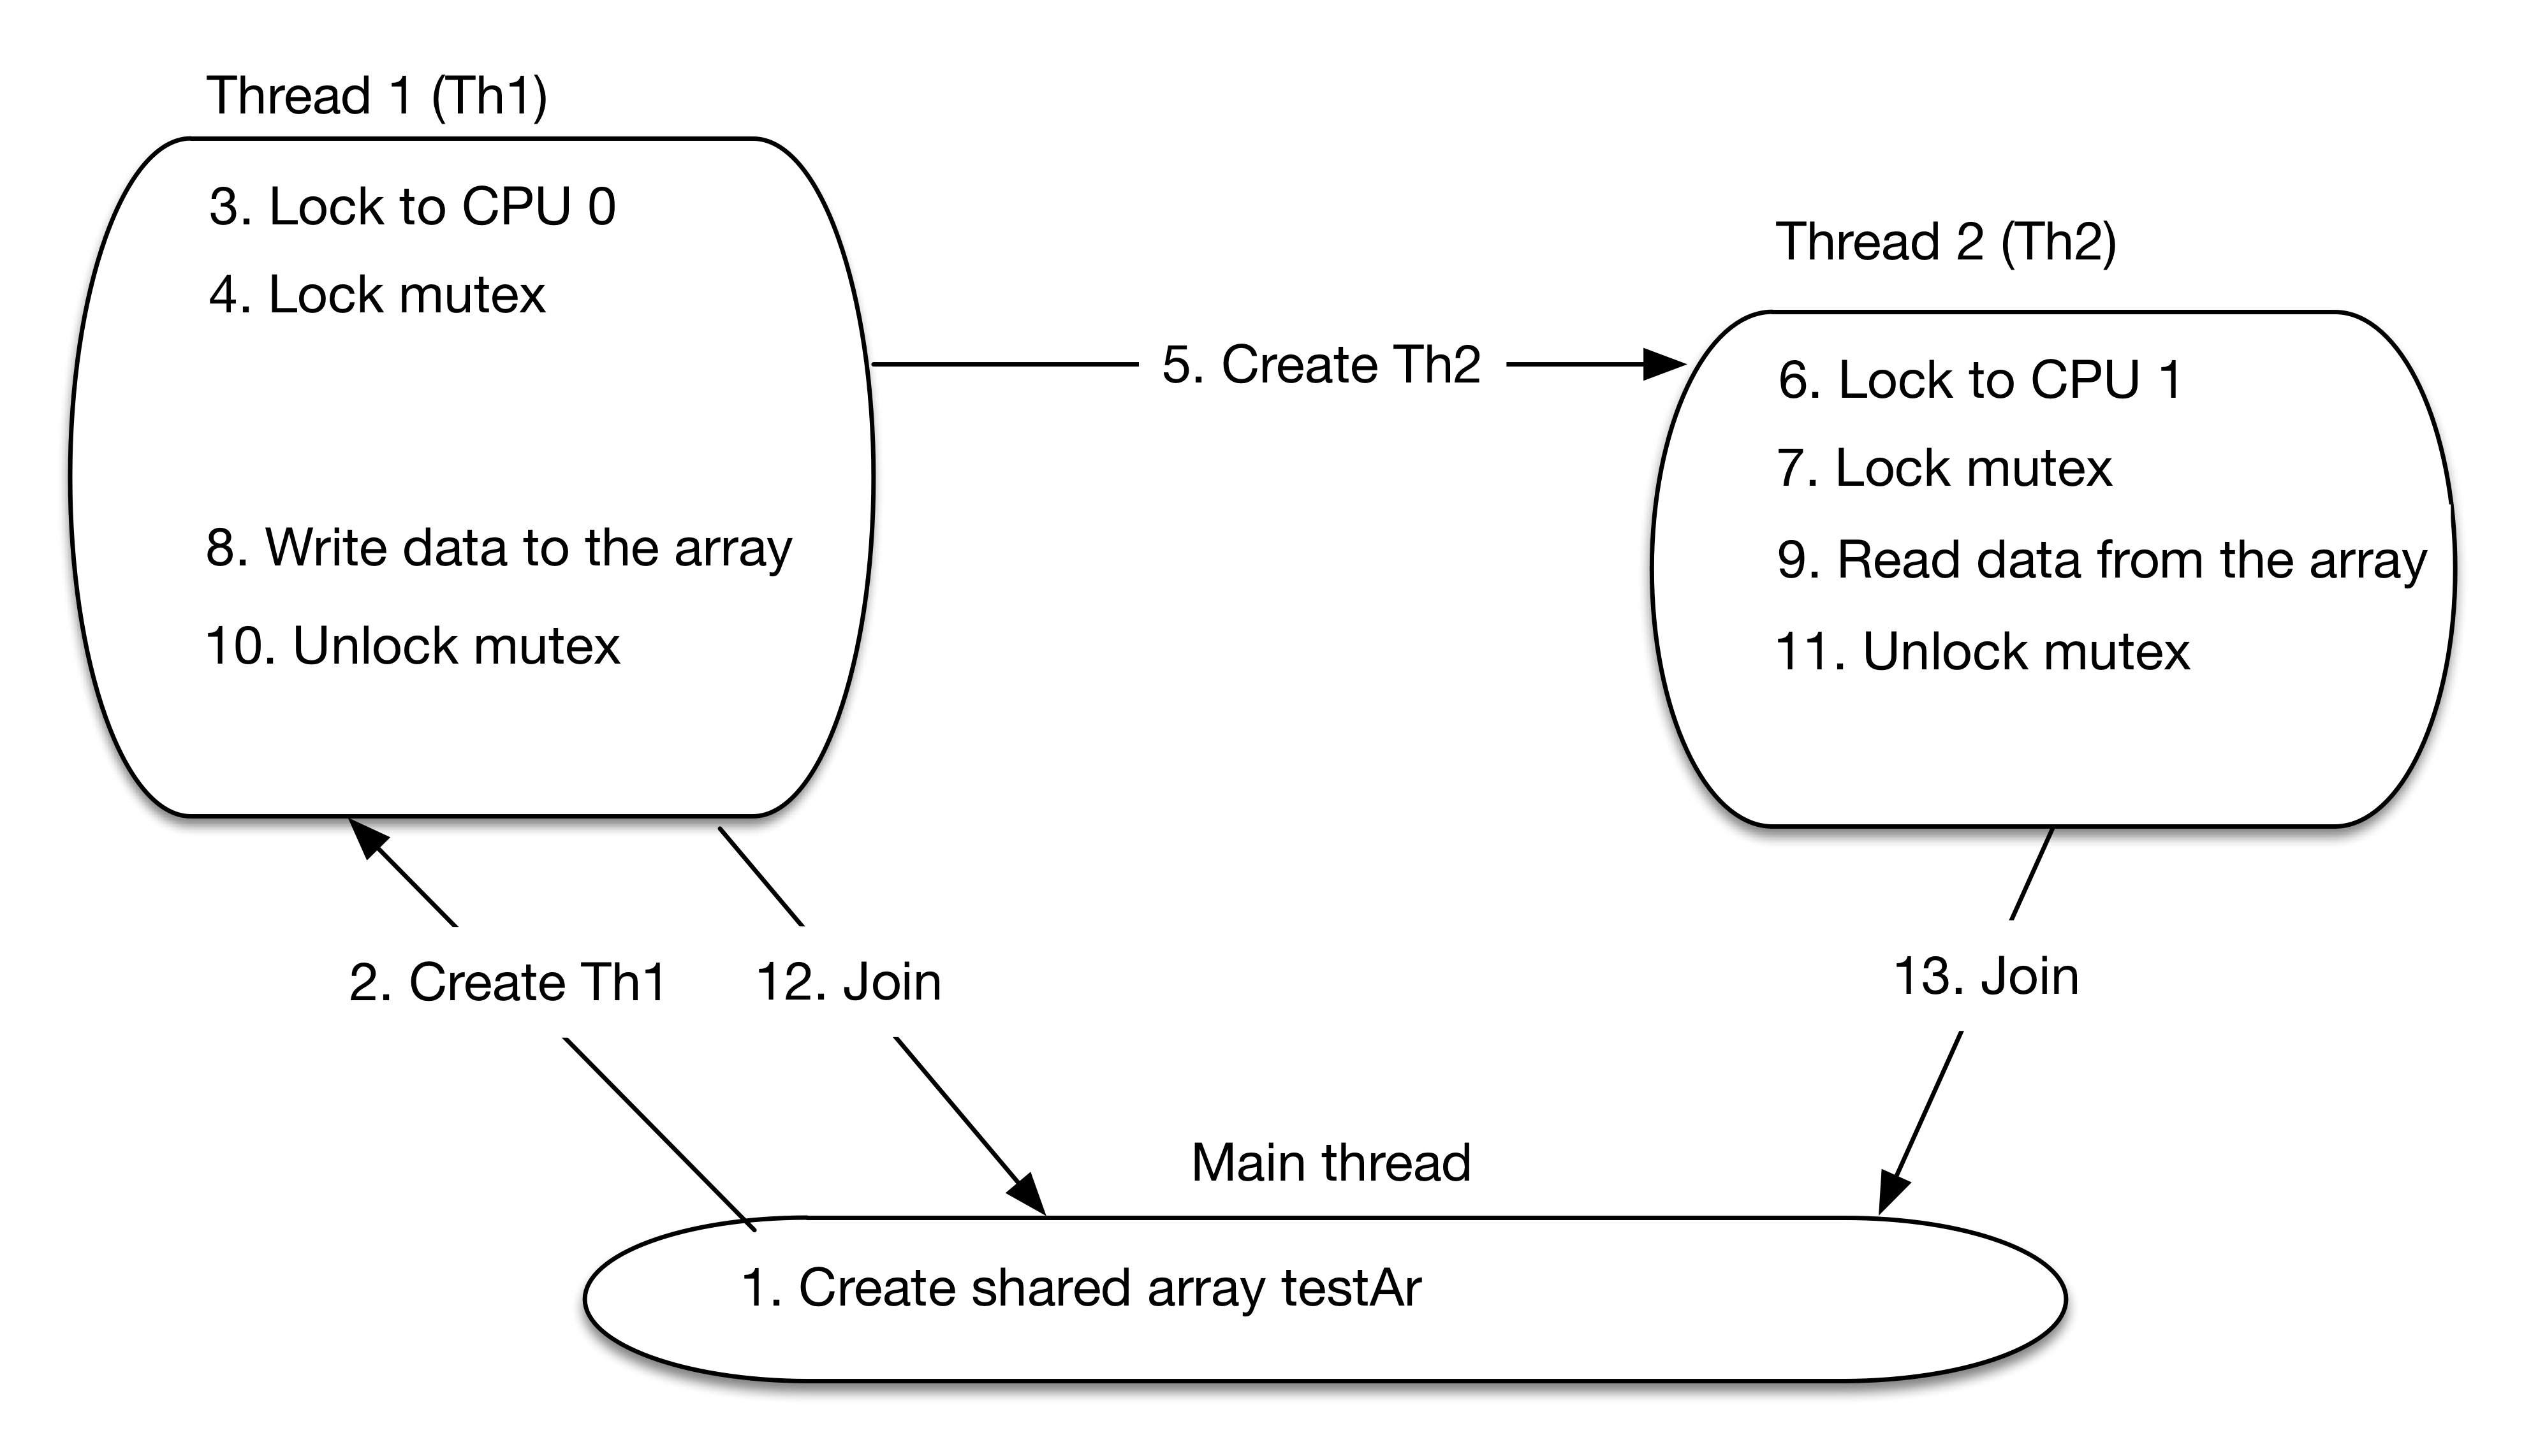
\includegraphics[width=145mm]{4/flow_threads_app_experiment.png}
\caption{A diagram showing the interactions between threads in Experiment 3}
\label{flow_threads_app_experiment}
\end{figure}

The first thread that plays a role of a writer is opened in the entry function, but, before it can be created certain, information needs to be wrapped in a structure so that it can be passed to a function that is to be executed from the new thread. Such ``walk-around" must be used because the \textit{pthread\_create()}\footnote{\url{http://man7.org/linux/man-pages/man3/pthread_create.3.html}} function that has to be called to create a new POSIX-thread can only take a single argument that can be passed to a function that is executed in the thread. Refer to a listing \ref{argStruct} for the definition of the structure. It stores the following information: 1) the ID of an experiment; 2) the size of data that is handled in the current iteration of the experiment; 3) a pointer to the array that is shared between threads.

\begin{lstlisting}[
language=C,
caption={A structure used to pass multiple arguments to the \textit{pthread\_create()} function},
label={argStruct}
]
/*
 * Structure used for a wrapper function used in pthread_create.
 */
struct argStructType {
	int experimentId; // ID of an experiment.
	int n; // Size of data handled in the experiment.
	long * testAr; // Pointer to a shared between
	               // threads structure.
};
\end{lstlisting}

The structure is passed to the thread where it is unwrapped at the entry to the function that is run in the thread \textit{void *e2\_pthread\_main1(void * argStruct)}; functions that are run from the writing threads in the Experiment 3 and the Experiment 4 are called \textit{void *e3\_pthread\_main1(void * argStruct)} and \textit{void *e4\_pthread\_main1(void * argStruct)} respectively. The mutex is then locked.

The second thread is created from the function that is run in the first thread \textit{void *e2\_pthread\_main2(void * argStruct)}; functions that are run from the reading threads in the Experiment 3 and the Experiment 4 are called \textit{void *e3\_pthread\_main2(void * argStruct)} and \textit{void *e4\_pthread\_main2(void * argStruct)} respectively. After that data is written into the shared array (by the first thread), and the mutex is unlocked in the first thread.

Similarly, the wrapped structure is passed to the second thread when it is created. The structure is unwrapped at the entry to the thread function, the mutex is then locked. Now when the mutex is locked and the first thread is prevented from accessing the shared data, contents of the shared array are read by the ``reader" (second) thread. The mutex is then unlocked in the second thread. Finally, both threads are joined by calling the \textit{pthread\_join()} function for each thread. Then, memory is freed and the mutex is destroyed.

\subsection{Organisation of Experiments}
The experiments are run with arrays up to $2^{24} * 8 = 134217728$ bytes (128 MB) in size. Such upper bound was chosen because it is larger than the Level 3 cache size in the Xeon E5-2695 v2, which is the size of the largest cache available across the systems used for executing the experiments. This figure is important because once the buffer contains more data that can fit into the largest cache, data is written into main memory, and caches no longer have impact on the speed of execution. Running experiments that share more data that can fit in the caches allows to measure latency of accessing main memory as well.

\begin{lstlisting}[
language=C,
caption={Function for choosing the length of an experiment},
label={listingCalculateN}
]
long calculate_n(long n) {
#ifdef MORE_EXPERIMENTS
    // Run a lot of experiments
	if (n < 100) {
		n *= 2.0;
	} else if (n > 100 && n < 1000) {
		n += 20;
	} else if (n > 1000 && n < 10000) {
		n += 200;
	} else if (n > 10000 && n < 100000) {
		n += 2000;
	} else if (n > 100000 && n < 1000000) {
		n += 20000;
	} else if (n > 1000000 && n < 10000000) {
		n += 200000;
	} else if (n > 10000000 && n < 100000000) {
		n += 2000000;
	} else {
		n *= 2.0;
	}
	return n;
#else
    // Or just multiple a number of bytes
    // in the iteration by two.
	return n * 2.0; 
#endif
}
\end{lstlisting}

The value of the only parameter -- the size of the array shared among threads -- is calculated in a function \textit{calculate\_n(long n)} that may be found in the file \textit{test\_env.c}\footnote{\url{https://github.com/Hollgam/cache-mt/tree/master/src/test\_env.c}}. This function ensures that samples of latency are taken uniformly. Refer to listing \ref{listingCalculateN} for a source code of that function. If a constant \textit{MORE\_EXPERIMENTS} is not defined, measurements are taken for the array of the size that is calculated as being a power of 2 (\textit{return n * 2.0}).

\begin{lstlisting}[
language=C,
caption={A function for assigning a thread to a particular processor core},
label={listingPinToCore}
]
// Pin thread to a particular core
int pin_thread_to_core(int coreId) {
	int num_cores = sysconf(_SC_NPROCESSORS_ONLN);
	if (coreId < 0 || coreId >= num_cores)
		return EINVAL;

	cpu_set_t cpuset;
	CPU_ZERO(&cpuset);
	CPU_SET(coreId, &cpuset);

	pthread_t current_thread = pthread_self();
	return pthread_setaffinity_np(current_thread,
	    sizeof(cpu_set_t), &cpuset);
}
\end{lstlisting}

A function \textit{int pin\_thread\_to\_core(int coreId)}\footnote{\url{https://github.com/Hollgam/cache-mt/tree/master/src/experiments.c}} for assigning threads to particular processor cores was also designed and developed. Refer to listing \ref{listingPinToCore} for a source code of the function. It utilises standard POSIX functionality that allows to receive a number of cores available in the system, such information is stored in a variable \textit{num\_cores}. A function \textit{pthread\_setaffinity\_np()} is then used to assign a current thread to a core with a given by a parameter \textit{coreId} core.

\section{Configuring Experimental Environment}
\label{design_env}

The rest of this chapter discusses common issues that are related to all experiments discussed in the previous section. A number of problems had to be faced while executing experiments. Solutions to these problems are outlined.

This section describes the experimental environment and outlines main difficulties that the author had to face to successfully run experiments and receive results that meet the requirements on precision and accuracy. The experimental environment can be configured by adjusting values in the file \textit{conf.h} \footnote{\url{https://github.com/Hollgam/cache-mt/tree/master/src/conf.h}}. A number of constants are declared in that file. By adjusting C's preprocessor macros that are defined in various places throughout the solution, one may configure the behaviour of the experimental environment.

All experiments are executed \textit{TIMES\_RUN\_EXPERIMENT} times. Each run of the experiment consists of a number of sub-experiments that are executions of the experiment with specific values given to the variable -- size of data shared between threads, if any -- that declares a number of times that each sub-experiment needs to be run. It is is defined by \textit{TIMES\_RUN\_SUB\_EXPERIMENT}. The values of these parameters were chosen through experimentation. Both of these values may be found in the \textit{conf.h} file.

\subsection{Avoiding Overhead from Operating System}
\label{OSinterference}

Both servers used in the study (refer to section \ref{sec_hardware}) work with Linux distributions. At the time of designing experiments, the server powered by Intel Xeon E5-2695 v2 processors\footnote{The server is referred as \textit{Xeon E5-2695 v2} in this document, unless stated otherwise.} was running SUSE Linux Enterprise Server 11\footnote{\url{https://www.suse.com/products/server/}}; the server based on Intel Xeon 5130\footnote{The server is referred as the \textit{Xeon 5130} in this document, unless stated otherwise.} was operated by Debian GNU/Linux 7\footnote{\url{https://www.debian.org/releases/wheezy/}}. Both of these distributions are identical in the areas that are relevant to this project, both of them are powered by the Linux kernel of version 3 (refer to table \ref{xeonTable}).

Before the design stage an alternative Operating System was also considered: BackTrack Linux\footnote{\url{http://www.backtrack-linux.org/}}. This version of Linux focuses on security and network and its authors claim that it is the ``highest rated and acclaimed Linux security distribution to date". Usage of this version of Linux can potentially present an environment with less overhead. The OS on the Xeon 5130 could be reinstalled; a number of tests with BackTrack Linux were performed by the author on his laptop, but no considerable advantages compared to Debian GNU/Linux 7 were found. The OS that powers Xeon E5-2695 v2 could not be altered, so a possibility of utilising a different Linux distribution for running experiments on that machine could not be considered.

The experimental environment is capable of setting the higher than default priority for the programme thread. It allows to eliminate overhead caused by the experiments being rescheduled by the scheduler. This is achieved with the \textit{setpriority} function\footnote{\url{http://linux.die.net/man/3/setpriority}} that sets the nice value\footnote{A \textit{nice} utility assigns a process with a particular priority, which gives the process either more or less CPU-time, compared to other processes registered in the system.} \cite{citeulike:200722} of the process. All experiments are assigned with higher than default priority. Refer to \ref{listingSetPriority} for the source code with the call of the function with passing appropriate arguments.

\begin{lstlisting}[
language=C,
caption={Setting higher priority of the process},
label={listingSetPriority}
]
int set_highest_process_priority(void) {
	setpriority(PRIO_PROCESS, 0, -20);
	return 1;
}
\end{lstlisting}

% Additionally, a possibility of running experiments as real-time processes \cite{Kernel.org2012} was investigated. However, it was learnt that such behaviour is not supported by the Xeon 5130 and enabling support for user-defined real-time processes would involve recompiling Linux with a modified kernel. It was decided that within the scope of the project such alteration of the OS would not be reasonable. The account that was used to run experiments on the Xeon E5-2695 v2 did not allow for such system-level changes to take place.

Then, a technique of \textit{warming up} cache was utilised in the experimental environment. The ``warm-up" is necessary to avoid receiving false data that is obscured by the interference of cache, as was learnt in the previous project \cite{Bazilinskyy2013}. Without the warm-up, incorrect time measurements would be received in the experiments, since caches would be have to be invalidated before being loaded with appropriate data. A few published papers were investigated, for example \cite{Luo2004}, but it was not possible to find a sufficient number of resources on the ways of performing cache warm-up ``intelligently". The authors of \cite{Luo2004} suggested using heuristics for the warm-up of caches in microprocessors. The heuristics is received by analysing the number of instructions in each sample of code. The proposed method for choosing heuristics is reasonable, but it was concluded that implementation of such technique would not give any noticeable advantage for running the relatively small-scale experiments designed within the scope of the project. The ``warm-up" is achieved by running one iteration of each experiment once before actually conducting the experiments, similarly to what is described in a much older publication \cite{D.Muntz1991}.

\begin{lstlisting}[
language=C,
caption={Alignment of data},
label={listingAlignmentData}
]
// Return a pointer to an aligned array of longs
long * align_long_array(int size) {
#ifdef ALIGN_DATA
    int cacheLine = 64 * 2;
	long x = malloc(size + cacheLine);
	if (x == NULL) { // Array for manipulating data
		printf("Error with allocating space.\n");
		exit(1);
	}
	return (unsigned long *) ((unsigned long long)
	    (x + cacheLine) & 0xFFFFFFE0);
#else
	return malloc(size);
#endif
}
\end{lstlisting}

Then, all data that is shared among threads and is used in the inter-thread communication is aligned on the initialisation stage. Alignment is done to prevent cache misses, which affect performance. Panda P.R. in his papers \cite{Panda1999} and \cite{RanjanPanda1997} together with other researchers discuss the method of alignment, which involves the insertion of ``dummy" data into allocated for a certain variable space. In this project a more simplified approach was taken, where a function receives a pointer to an array of type \textit{long} and simply aligns it by a number of bytes that correlate to the size of one cache line. Refer to listing \ref{listingAlignmentData} for a snippet of C code that performs alignment of data on both the Xeon 5130 and the Xeon E5-2695 v2s. A preprocessor directive \textit{\#ifdef ALIGN\_DATA} checks if a global variable \textit{ALIGN\_DATA is defined}, which indicates that alignment of data must be performed.

Finally, \textit{-O0} flag is used when experiments are compiled with the \textit{gcc} compiler. It ensures that the lowest level of compiler optimisation is used.

\subsection{Measuring Interrupts and Minor and Major Page Faults}

There are a number of sources of inaccuracy of time measurements. To eliminate the overhead imposed by them, the occurrence of the following events is monitored by the experimental environment: minor and major page faults and interrupts. The occurrence of context switches is not traced because, as was learnt, they always occur when interrupts take place. None of these events are desired as all of them take relatively long time to execute and can potentially make low-level experiments invalid.

A page fault can occur when a CPU attempts to access a page that resides in the virtual address space, but cannot be found in physical memory. Such events are normally handled by the memory management unit (MMU) making the required page accessible in physical memory. Attempts to access pages that do not exist are tolerated as ``illegal access errors" and may result in the termination of a programme. There are two types of page faults: minor and major. Minor page faults occur when the page is loaded into physical memory, but the MMU has not marked it as being in the physical memory space. Major page faults happen when the CPU tries to access an address in virtual memory that does not have a page in physical memory assigned to it. The reference to a missing page causes the OS kernel to allocate a page and return back to the MMU. Major page faults have extremely negative impact on the performance of the system, they are much more expensive than minor page faults and they increase latency of memory access dramatically. \cite{rao2008computer}

Another process that regularly takes place in modern-day computers is an interrupt. It is a signal that is emitted when a certain event needs immediate attention and CPU-time. Such high-priority events demand currently executed tasks to be interrupted and scheduled for later execution. When such activity happens, a CPU saves its state and executes an interrupt handler \cite{Mogul1997}. After the interrupt handler finishes its execution, the CPU can continue with execution of the thread that had to be stopped. Interrupts take noticeable amount of time to be finished and can obscure results of experiments that require high precision. A number of different types of interrupts can occur in the system. Time interrupts can be seen each time the internal clock reaches a certain value.

Lastly, a context switch (also known as a task switch) is the switching of the central processing unit from one thread to another. In other words, a context switch\footnote{\url{http://www.linfo.org/context_switch.html}} is a process of the kernel suspending execution of one process and resuming execution of another process that had previously been put on pause. Context switches as well as all aforementioned processes affect multi-threaded programmes \cite{agarwal1992performance}.

An experiment is thought to be invalid if any page faults or interrupts (and consequently context switches) take place during the run of the experiment. Time measurements in such experiments cannot be accurate. One minor page fault per file that is read before starting an experiment is allowed: such page faults rise because of operations that the OS performs when files are read with the \textit{fopen()}\footnote{\url{http://man7.org/linux/man-pages/man3/fopen.3.html}} function. No sources that document such behaviour were found, hence it was proven experimentally with a program \textit{test\_pagefault\_fopen}\footnote{\url{https://github.com/Hollgam/cache-mt/blob/master/test\_pagefault\_fopen/pagefaults\_fopen.c}}. Refer to appendix \ref{app:listingTestPagefault} for the source code of the programme. The output of the programme run on the Xeon 5130 may be seen in a listing \ref{listingOutputPageFaultOpen}.

\begin{lstlisting}[
language=bash,
caption={Results from the experiment that proves that one minor page fault is generated per file-read},
label={listingOutputPageFaultOpen}
]
1st time /proc/interrupts: Before: 209 After: 220
2nd time /proc/interrupts: Before: 222 After: 223
1st time /proc/iomem: Before: 224 After: 225
2nd time /proc/iomem: Before: 226 After: 227
/proc/interrupts changed: Before: 241 After: 244
\end{lstlisting}

The programme \textit{test\_pagefault\_fopen} reads files \textit{``/proc/interrupts"} and \textit{``/proc/iomem"}, which are generated by the Linux kernel and are heavily used in this project. A number of page faults generated across the system is read once before a file is read (written as a number after ``Before:" in the output) and straight after the file is closed (written as a number after ``After:" in the output). A thesis that page faults are generated only after files are read for the first time was suggested. To check this assumption, both files used in the experiments are read twice (results measured when the file is read for the 1$^{\textnormal{st}}$ time are marked with ``1st time", when the file file is opened for the 2$^{\textnormal{nd}}$ time in the same session -- ``2nd time"). The experiment showed that it is not a case. Additionally, a different scenario was tested: when files are changed by the OS between taking measurements of generated page faults. The results from testing this scenario are presented in the last line of the output: three page faults are generated for the file \textit{``/proc/interrupts"}; however, this figure is not constant for different files. A decision was made to disregard results from running experiments where more page faults are generated than a number of files read for measuring data before the start of the experiment.

A number of interrupts that occur during the execution of an experiment is derived by subtracting a sum of all interrupts registered in the system before running the experiment from a sum of all interrupts that can be measured after the experiment has finished. A number of interrupts can be obtained by reading a system file \textit{``/proc/interrupts"} that is generated dynamically on request by the kernel of the OS.

A similar logic is applied to obtaining numbers of page faults (both minor and major) that occur during the execution of experiments: first, one measures a number of page faults that occurred while running an experiment before the execution of the test, then after the experiment has finished. Then, a number of page faults generated before running the experiment is subtracted from a figure that is read after the experiment is no longer running. Such information is generated for each process that is run by Linux individually and may be found in a file \textit{``/proc/PID/stat"}, where \textit{PID} indicates the ID of a process.

The files \textit{``/proc/interrupts"} and \textit{``/proc/PID/stat"} need to be opened for reading information about the numbers of interrupts and page faults recorded prior to running an experiment. The content of these two files is stored in variables of type \textit{char *} and it is read after finishing the experiment. It is done in this way to avoid overhead caused by the analysis of the content of the files for fetching figures of detected interrupts and page faults. Furthermore, before all experiments are run, the content of the files is stored into two ``extra" \textit{char *} variables each time before reading data from them. Such operation is maintained to avoid possible compiler optimisation that may generate additional page faults and prevent receiving accurate results.

\begin{lstlisting}[
language=C,
caption={Measuring time after timer tick or after recording a timer interrupt},
label={listingStartMeasuringTime}
]
#if START_AFTER == TIMER_TICK
	// Start after the timer ticks.
	struct timespec temp_time1, start;

	get_time_ns(&temp_time1);
	get_time_ns(&start);

	while (start.tv_sec == temp_time1.tv_sec &&
	    temp_time1.tv_nsec == start.tv_nsec) {
		get_time_ns(&start);
	}
#elif START_AFTER == TIME_INTERRUPT
	// Start after the time interrupt
	unsigned long long interrupts1 = search_in_file(
	    "/proc/interrupts", "LOC:", 1);
	unsigned long long interrupts2 = search_in_file(
	    "/proc/interrupts", "LOC:", 1);

	while (interrupts1 == interrupts2) {
		interrupts2 = search_in_file(
		    "/proc/interrupts", "LOC:", 1);
	}
	// Calculate the start time
	struct timespec start;
	get_time_ns(&start);
#endif
\end{lstlisting}

To further eliminate a possibility of the Operating System altering the timing results, a number of other precautions were taken. All experiments may be started after a timer tick or after a timer interrupt is recorded in the system. The listing \ref{listingStartMeasuringTime} shows a piece of code in the experimental environment that is responsible for taking a timestamp before running an experiment.

\section{Timing}

\subsection{Measuring Time at Nano-Second Accuracy}
\label{measuringTime}

One of the most challenging aspects of designing the experimental environment for running the experiments that are described in this document was finding a way to measure execution times with enough precision, at a nano-second level. Time can be measured in either nano-seconds or clock cycles\footnote{\textit{Clock cycle} is the amount of time between two adjacent pulses of a processor oscillator.}. A number of options were found and evaluated. This section describes two approaches that were considered.

\subsubsection{Using clock\_gettime(3)}

The first tool that was evaluated for measuring time was the \textit{clock\_gettime(3)}\footnote{\url{http://linux.die.net/man/3/clock_gettime}} function that is provided in most Linux kernels. It is a monotonic function. It is said to be capable of providing measurements of time with nano-second accuracy. The figures of recorded seconds and nano-seconds are stored separately in two 32-bit counters, hence a ``wrap-around" may happen only after many years of the execution time.

The documentation says that \textit{CLOCK\_MONOTONIC} provides ``Clock that cannot be set and represents monotonic time since some unspecified starting point". In other words, it represents the absolute amount of time elapsed since a certain fixed point in the past. It is not affected by the system's clock. \textit{CLOCK\_REALTIME} was also experimented with, but it proved to be less reliable. The reading generated by this clock can be affected by discontinuous jumps in the system time (e.g. the clock is adjusted manually).

The documentation\footnote{\url{http://linux.die.net/man/3/clock_gettime}} associated with this function states that it provides highly-accurate results with nano-second precision. A function \textit{get\_res(3)} was used to find the precision of \textit{clock\_gettime(3)} and, indeed, in cases of both machines utilised in the study \textit{clock\_gettime(3)} does support nano-second precision.

No tools are offered to test the accuracy of this function. A custom programme to check the accuracy of \textit{clock\_gettime(3)} was developed. The application \textit{test\_clockgettime}\footnote{\url{https://github.com/Hollgam/cache-mt/blob/master/test\_clockgettime/clock-gettime\_test.c}} was written to learn whether the amount of overhead of running this function is constant, i.e. if it is capable of outputting the same amount of nano-seconds when the same experiment is run multiple times in the same environment setting. Refer to appendix \ref{app:listingTestClockGetTime} for the source code of the programme. This programme calls \textit{clock\_gettime(3)} 1024 times and records what is returned by the function in each case in an array. Then, it outputs differences between the i$^{\textnormal{th}}$ and the (i-1)$^{\textnormal{th}}$ calls. Refer to \ref{lst:clock_gettime} for an excerpt of the output generated by this programme.

\begin{lstlisting}[
language=bash,
caption={An excerpt from running the \textit{test\_clockgettime} programme on the Xeon 5130},
label={lst:clock_gettime}
]
clock_gettime() ==
90 85 81 81 81 81 82 84 81 81 81 82 81 84 81 81 82 81 81 84 81
82 81 81 81 84 82 81 81 81 81 85 81 81 81 81 82 84 81 81 81 82
81 84 81 81 82 81 81 84 81 82 81 81 81 84 82 81 81 81 81 85 81
81 81 81 82 84 81 81 81 82 81 84 81 81 82 81 81 84 81 82 81 81
81 85 81 81 81 81 82 84 81 81 81 82 81 84 81 81 82 81 81 84 81
82 81 81 81 84 82 81 81 81 81 85 81 81 81 81 82 84 81 81 81 82
81 84 81 81 82 81 81 84 81 82 81 81 81 84 82 81 81 81 81 (...)
\end{lstlisting}

As may be noticed, unfortunately, \textit{clock\_gettime(3)} did not output the same result each time it was called in the testing application. It may be explained by the fact that different underlying instructions may take different amounts of clock-cycles in modern-day CPUs \cite{Granlund2012}. Hence this function cannot be fully trusted for timing experiments that demand high precision. Further, this function uses the \textit{RDTSC} high-frequency timer in its core, so a more direct approach to use that function straight away was considered as an alternative. The overhead of running \textit{clock\_gettime(3)} is also quite large and is equal to 81 -- 90 nano-seconds, which is a big disadvantage of this method.

\subsubsection{Using RDTSC/RDTSCP}

Due to instability of \textit{clock\_gettime(3)} and a relatively large amount of overhead that is associated with calling that function, the \textit{Read time-stamp counter} (RDTSC)\footnote{\url{http://www.mcs.anl.gov/~kazutomo/rdtsc.html}} instruction was chosen as an alternative way to time the experiments. It is an instruction that on x86 and x86-64 platforms can access the Time Stamp Counter (TSC) 64-bit register. As with \textit{clock\_gettime(3)}, the issue of the number reported by \textit{RDTSC} ``wrapping around" is close to being non-existent. The \textit{RDTSC} instruction always returns an increased number until it wraps around. However, in case of, for example, a 2 GHz processor, such behaviour can be seen only after about three centuries.

\begin{lstlisting}[
language=C,
caption={The wrapper function for calling RDTSC with Assembly language},
label={lst:func_rdtsc}
]
/*
 * Use RDTSC to measure time at nanosecond
 * accuracy (if it is not disabled)
 * CPUID == 1 - use CPUID;
 * CPUID == 0 - do not use CPUID.
*/
unsigned long long rdtsc(int CPUID) {
	unsigned long a, b;
	unsigned long long temp;
	if (CPUID)
		__asm__ __volatile__("CPUID\nrdtsc" : "=a" (a),
		    "=d" (b):: "memory", "%ebx", "%ecx");
	else
		__asm__ __volatile__("rdtsc" : "=a" (a),
		    "=d" (b):: "memory", "%ebx", "%ecx");
	temp = b;
	temp = (temp << 32) | a;
	return temp;
}
\end{lstlisting}

\textit{RDTSC} is an Assembly command that loads the current value of the processor's time-stamp counter into the EDX:EAX registers \cite{Faydoc2014}. A wrapper function that calls a piece of inline Assembly code was written. Refer to \ref{lst:func_rdtsc} for a listing with a source code of the function. This function has a single parameter \textit{int CPUID}, which is a flag that indicates whether \textit{CPUID} instruction should be called before invoking the \textit{RDTSC} operation. This instruction is called before \textit{RDTSC} because it prevents out-of-order execution on modern CPUs (a situation when instructions are executed in a different than was programmed order). Invocation of the \textit{CPUID} command serializes the instruction queue. 

The author of \cite{Kankowski2012} states that a combination of \textit{CPUID} and \textit{RDTSC} can provide constant performance, i.e. the overhead associated with invoking these commands is constant. A function \textit{void test\_rdtsc(void)}\footnote{\url{https://github.com/Hollgam/cache-mt/blob/master/test/src/hr\_timer.c}} was built to verify this thesis. Refer to appendix \ref{app:listingTestRDTSC} for a source code of the function. Similarly to the test that was performed to verify the accuracy of \textit{clock\_gettime(3)}, this program calls \textit{RDTSC} 1024 times. Refer to figure \ref{lst:test_rdtsc} for an excerpt from the output of this application when it was run on the Xeon 5130. It outputs what is received from the instruction: large numbers (e.g. 21210592467695670), which represent the amount of ellapsed time. The numbers in square brackets indicate the differences with what was returned from the previous calls of the \textit{RDTSC} instruction (e.g. [336]). Despite what is claimed in \cite{Kankowski2012}, this excerpt clearly shows that RDTSC is not capable of providing constant performance on the Xeon 5130, the test was also executed on the Xeon E5-2695 v2, but the results were largely the same: the overhead was not constant. It may be a case because of the nature of underlying Assembly-commands that take different numbers of clock-cycles to execute on modern CPUs. Any other more reliable sources of information on the nature of \textit{RDTSC} and its performance could not be found.

\begin{lstlisting}[
language=bash,
caption={An excerpt from running the \textit{test\_rdtsc()} function on the Xeon 5130},
label={lst:test_rdtsc}
]
21210592467695670 [336]
21210592467695994 [324]
21210592467696318 [324]
21210592467696642 [324]
21210592467696972 [330]
21210592467697296 [324]
21210592467697626 [330]
21210592467697950 [324]
21210592467698274 [324]
21210592467698604 [330]
21210592467698928 [324]
21210592467699252 [324]
21210592467699594 [324]
21210592467699918 [324]
21210592467700242 [324]
21210592467700566 [324]
21210592467700890 [324]
21210592467701220 [330]
(...)
\end{lstlisting}

The aforementioned test showed that receiving accurate timing information with assistance of RDTSC is a complicated undertaking on its own. In addition to the problem of out-of-order execution of instructions on modern-day CPUs (like those that are used in the study), the clock speed also varies, which leads to the alteration of timing results. In older multi-core systems, the rate returned by \textit{RDTSC} could change differently on different execution units, as they would adjust their clock speeds according to the load.

Another possibility was suggested in one of the white paper from Intel on this topic \cite{Paolini2010}: the \textit{RDTSCP} instruction. The main difference between \textit{RDTSCP} and the standard \textit{RDTSC} instructions is that \textit{RDTSCP} works as a serializing instruction, i.e. the CPU is prevented from reordering instructions around the call to \textit{RDTSCP}. Unfortunately, \textit{RDTSCP} is available only on new processors, and a number of tests showed that it could not be run in the experimental environment designed for this project.

\section{Support for Mac OS}

Because a machine powered by Mac OS X could be easily accessed, this Unix-based OS was also selected as a platform for running the experiments. Most functionality that is supported by Linux is also available in Mac OS. This assumption was not valid in case of the \textit{clock\_gettime(3)} function. A custom-built timer that imitates the behaviour of \textit{clock\_gettime(3)} was designed and developed in the early stage of this project to extend support of Mac OS. Its implementation may be found in the file \textit{clock\_gettime\_mac.c}\footnote{\url{https://github.com/Hollgam/cache-mt/tree/master/src/clock\_gettime\_mac.c}}.

It was speculated that the author's MacBook Air laptop powered by an Intel i7 processor could also be used for running experiments. Then at a much later stage of the project the fact that Mac OS does not support assigning threads to particular cores was discovered. The initial vision of the experimental environment assumed that it would be cross-platform and could be used for running experiments on both Linux-based systems and on Mac OS X. After it was learnt that such vital for the success of the project functionality cannot be achieved by using the standard tools offered on Mac OS, a decision to abandon the cross-platform support was taken. As a result, the proposed system is only partially cross-platform.

\section{Measuring Duration of Interrupts and Minor Page Faults}
\label{design_duration_int_pf}

It is important to know the duration of one time interrupt and a minor page fault, since these events have a big affect on performance of a system that is engaged in inter-thread communication. At first an attempt to retrieve information about the values of duration of page faults, context switches, and interrupts was undertaken. No such data was found for both CPUs used in the experiments.

A programme for testing the duration of an interrupt \textit{test\_time\_int\_pf}\footnote{\url{https://github.com/Hollgam/cache-mt/tree/master/test\_time\_int\_pf}} was written. Refer to appendix \ref{app:listingTestInterrupt} for a listing of the source code of the main function that handles the experiment. Most supplementary functions that handle measuring time and getting information on the numbers of recorded interrupts and page faults are described in this chapter. This application waits until an interrupt is detected and measures a difference between timestamps taken before and after occurrence of the interrupt. Such operation is performed 10 times. Similar actions are taken to record the duration of a minor page fault. Then, the average duration of one interrupt is reported.

\section{Dependability}
\label{dependabilitySection}

This section discusses the aspect of dependability of the proposed solution. This thesis focuses on the impact of cache on data-intensive multi-threaded application. Programmes of this type often have high requirements for security and protection of data: separation of bandwidth in telecommunication systems, accessing data in distributed databases, etc. Speed is an important factor for achieving stable performance of such systems, and the impact of the cache needs to be predictable and quantifiable.

The outlined in the section experiments run directly on the hardware. Execution times are measured by extracting information straight from CPU registers. Therefore, measured data is dependable, provided that the used hardware does not malfunction. Boolean logic is used to test modern-days microprocessors and the probability of using a faulty processor is very small, as the fault tolerance of CPUs is extremely high. Two processors were used to run the experiments, one of which powers a supercomputer in a respected research institute, so the chance of operating a faulty processor becomes even lower.

All experiments were run ten times and the final results are generated from calculating the average values from all runs of the experiments. Moreover, special care was taken to avoid interference from the OS by detecting interrupts and page faults, warming up caches, and starting each experiment after a timer tick / interrupt is recorded.
% ---------------------------------------------------------------------------
%: ----------------------- end of thesis sub-document ------------------------
% ---------------------------------------------------------------------------

	
% this file is called up by thesis.tex
% content in this file will be fed into the main document

%: ----------------------- name of chapter  -------------------------
\chapter{Conducting Experiments} % top level followed by section, subsection
\label{chapterCondExp}

%: ----------------------- paths to graphics ------------------------

% change according to folder and file names
\ifpdf
    \graphicspath{{X/figures/PNG/}{X/figures/PDF/}{X/figures/}}
\else
    \graphicspath{{X/figures/EPS/}{X/figures/}}
\fi

%: ----------------------- contents from here ------------------------

This chapter gives an outline of the process of conducting cycle- and application-level experiments that are described in the previous chapter. It provides a detailed description of what needs to be done to run the described experiments on the Xeon 5130 and Xeon E5-2695 v2 processors. If a reader wishes to replicate the study, the content of this chapter will give a detailed description on how to do that. It starts from giving a description of the hardware that was used in the project. It also lists main constraints that had to be faced while running the experiments.

\section{Hardware}
\label{sec_hardware}

The faculty of Computer Science in the National University of Ireland, Maynooth provided access to a machine powered by one Intel Xeon 5130 dual-core processor. Rights to SSH into the computer and use it for this research were also given. Additionally, the Ireland's High-Performance Computing Centre (ICHEC)\footnote{\url{https://www.ichec.ie/}} offered to create an account on their fionn3 server. That server has 320 nodes (7680 cores; 20 TiB RAM) and each node contains 24 (2x12) Ivy Bridge CPU cores that are powered by Intel Xeon E5-2695 v2 CPUs. Fundamentally, the processors utilised in the machines are similar, but they exhibit different levels of support to varies technologies. For example, the Xeon E5-2695 v2 supports the \textit{RDTSCP} instruction, and the Xeon 5130 does not. Moreover, Intel Xeon 5130 is 7 years older than Intel Xeon E5-2695 v2 and they have a number of vital differences. Such differences are beneficial for the analysis of results obtained in the project. A table \ref{xeonTable} outlines main characteristics of both machines.

\begin{table*}
\caption{Description of the processors used in the study}
\centering 
\begin{tabular}{lll}
\hline
                & \textbf{Intel Xeon 5130 (NUIM)} & \textbf{Intel Xeon E5-2695 v2 (ICHEC)} \\ \hline
Server          & IBM System x3550 -[797841Y]-                     & Fionn\footnote{\url{https://www.ichec.ie/infrastructure/fionn}}                       \\
Launch year     & 2006                       & 2013                             \\
Lithography     & 65 nm                      & 22 nm                            \\
Number of cores & 4                          & 24                               \\
Clock speed     & 2 GHz                      & 2.4 GHz                          \\
L1 cache size   & 32 KB                      & 32 KB                            \\
L2 cache size   & 4 MB                    & 256 KB                           \\
L3 cache size   & None                       & 30 MB \\
Cache line size   & 64 B                       & 64 B \\
Linux version   & 3.2.0-4-rt-amd64           & 3.0.74-0.6.6-default
\end{tabular}
\label{xeonTable}
\end{table*}

No CPU-specific specification for both processors used in the study (e.g. cache latency times) is available from Intel. The publicly-available software developer manual (especially chapter 11 in that document) was used for reference \cite{Intel2014}. Through experimentation and referring to a resource that discusses CPUs from the Intel Xeon 5600 processor family with a similar to what is used in the study architecture \cite{Balakrishnan2010}, layout diagrams were produced for both the Xeon 5130 and the Xeon E5-2695 v2. The figure \ref{Threads_cpu_diagram} outlines the design of the Intel Xeon 5130 processor. This is a multi-chip processor that has two CPUs. All cores have private Level 1 caches, all chips have private Level 2 caches. This processor does not have a shared Level 3 cache. Two chips are connected by a QPI (QuickPath Interconnect) point-to-point processor interconnect bus \cite{Intel2009a}.

\begin{figure}[ht!]
\centering
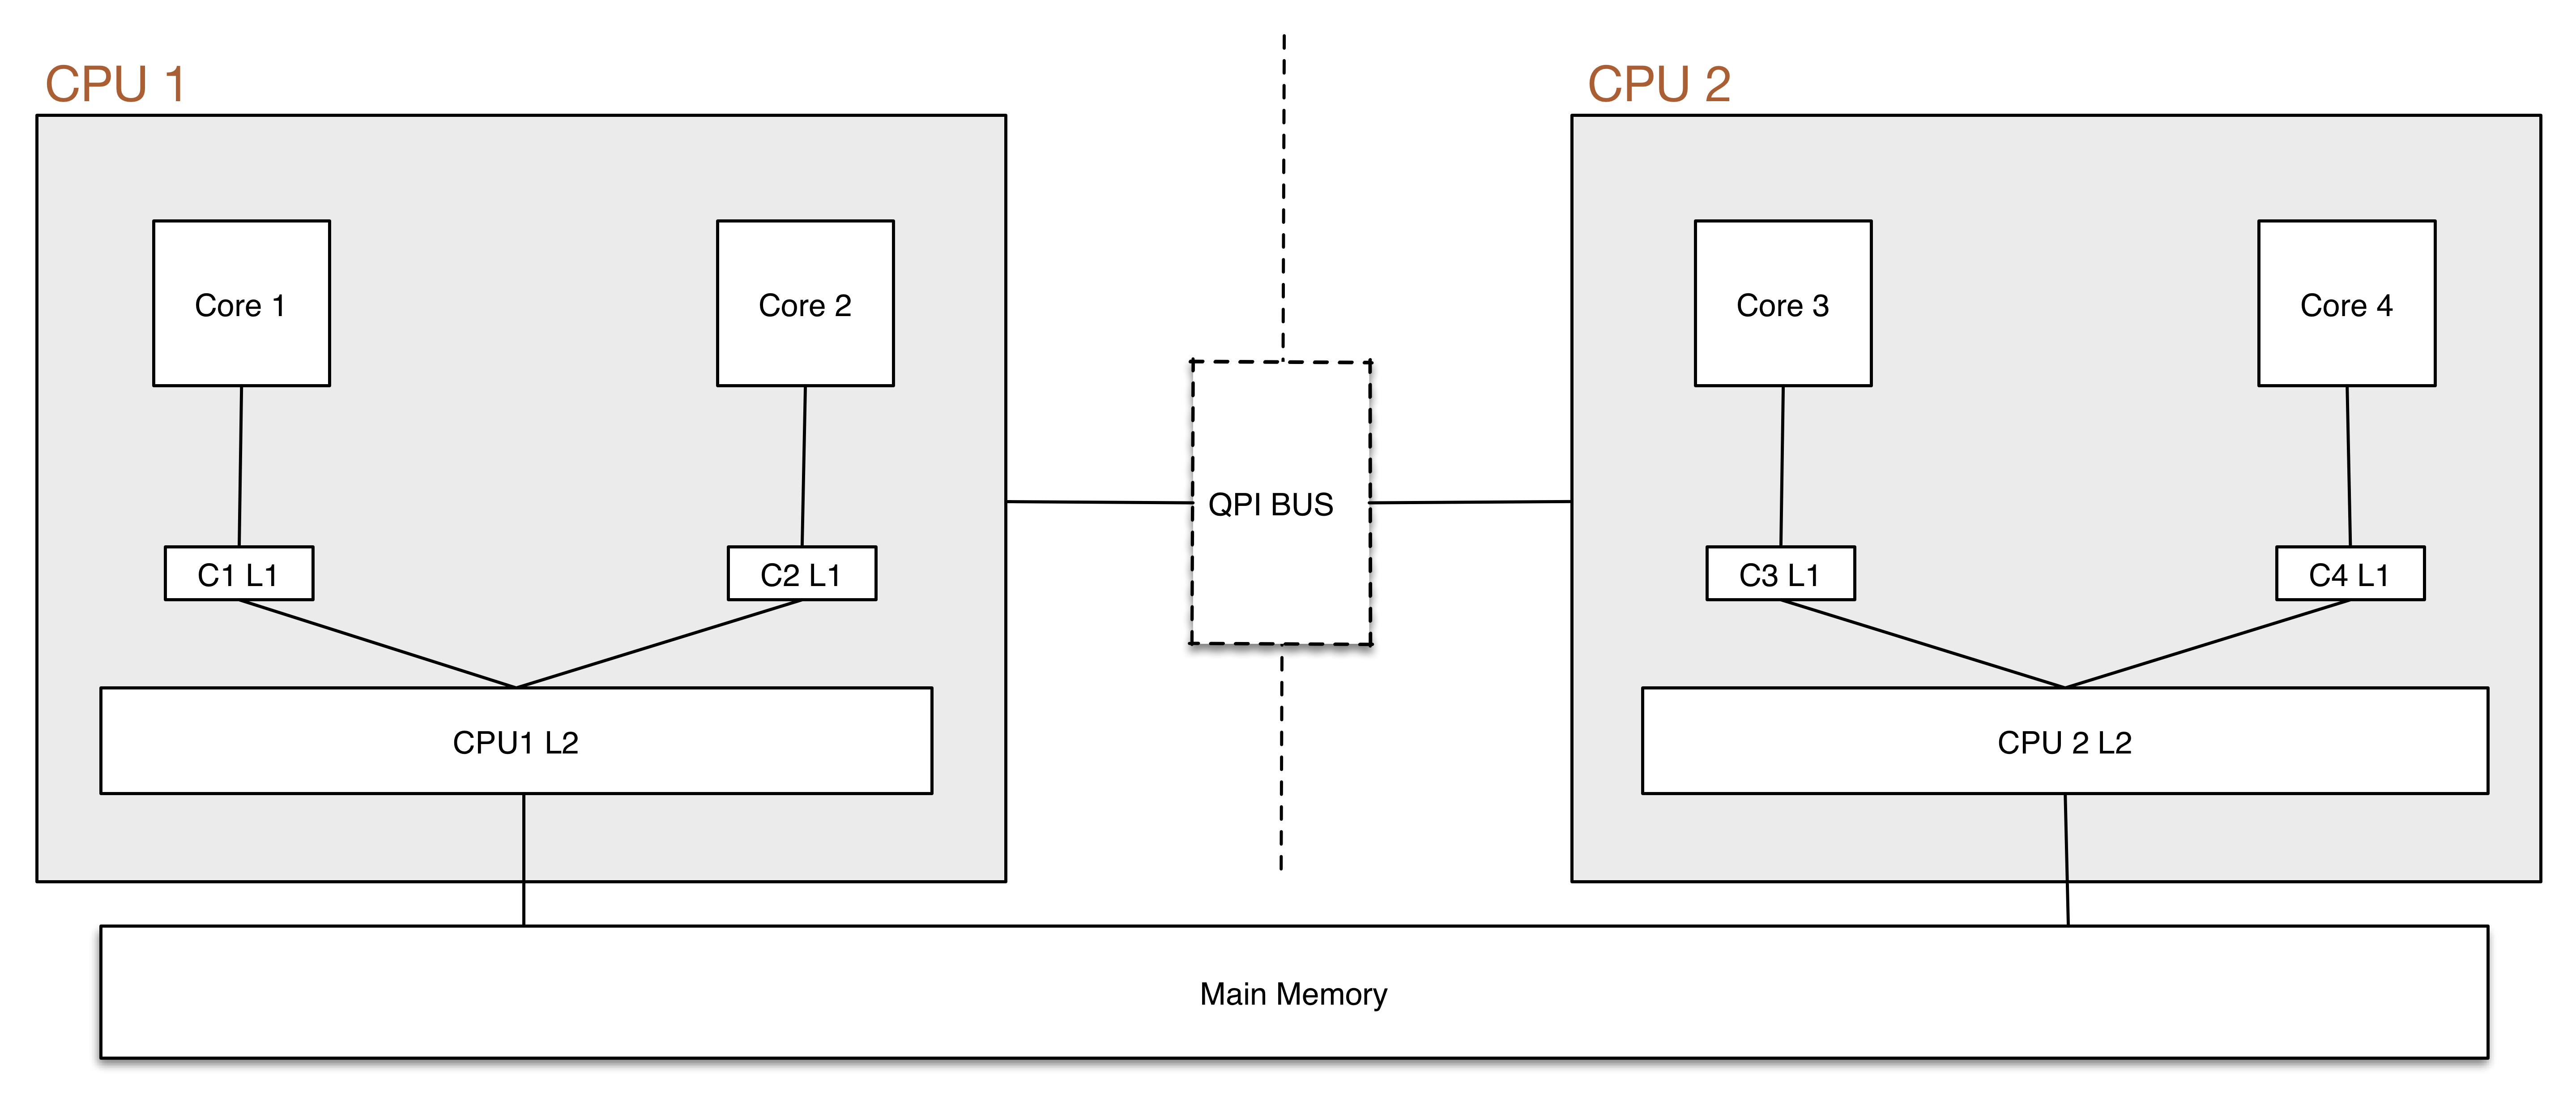
\includegraphics[width=145mm]{4/Xeon_5130.png}
\caption{Diagram of the layout of Xeon 5130}
\label{layout_xeon_5130}
\end{figure}

The diagram \ref{layout_xeon_2695} represents all main components of the Intel Xeon E5-2695 v2 CPU. This CPU has 24 cores, each core has private L1 and L2 caches, each of two dies has a rather big 30 MB L3 cache. The cores of this processor are also connected by a QPI bus.

In both cases the write-through (WT) cache is considered. Obtaining the exact figures for latency and throughput of different caches that are used in these processors, that can be supported by a published resource, proved to be impossible. The only official document from Intel \cite{Levinthal} that could be found reports latency for the processor Core i7 and the processor family Xeon 5500. The Xeon 5500 CPU is relatively similar to the Xeon 5130, yet it is three years newer and it works on much higher frequencies and instead of two cores it includes up to four hyper-threaded cores \cite{Intel2009}. The cache itself is fundamentally different, as processors of that type have Intel® Smart Cache-enabled caches \cite{Intel2012}.

\begin{figure}[ht!]
\centering
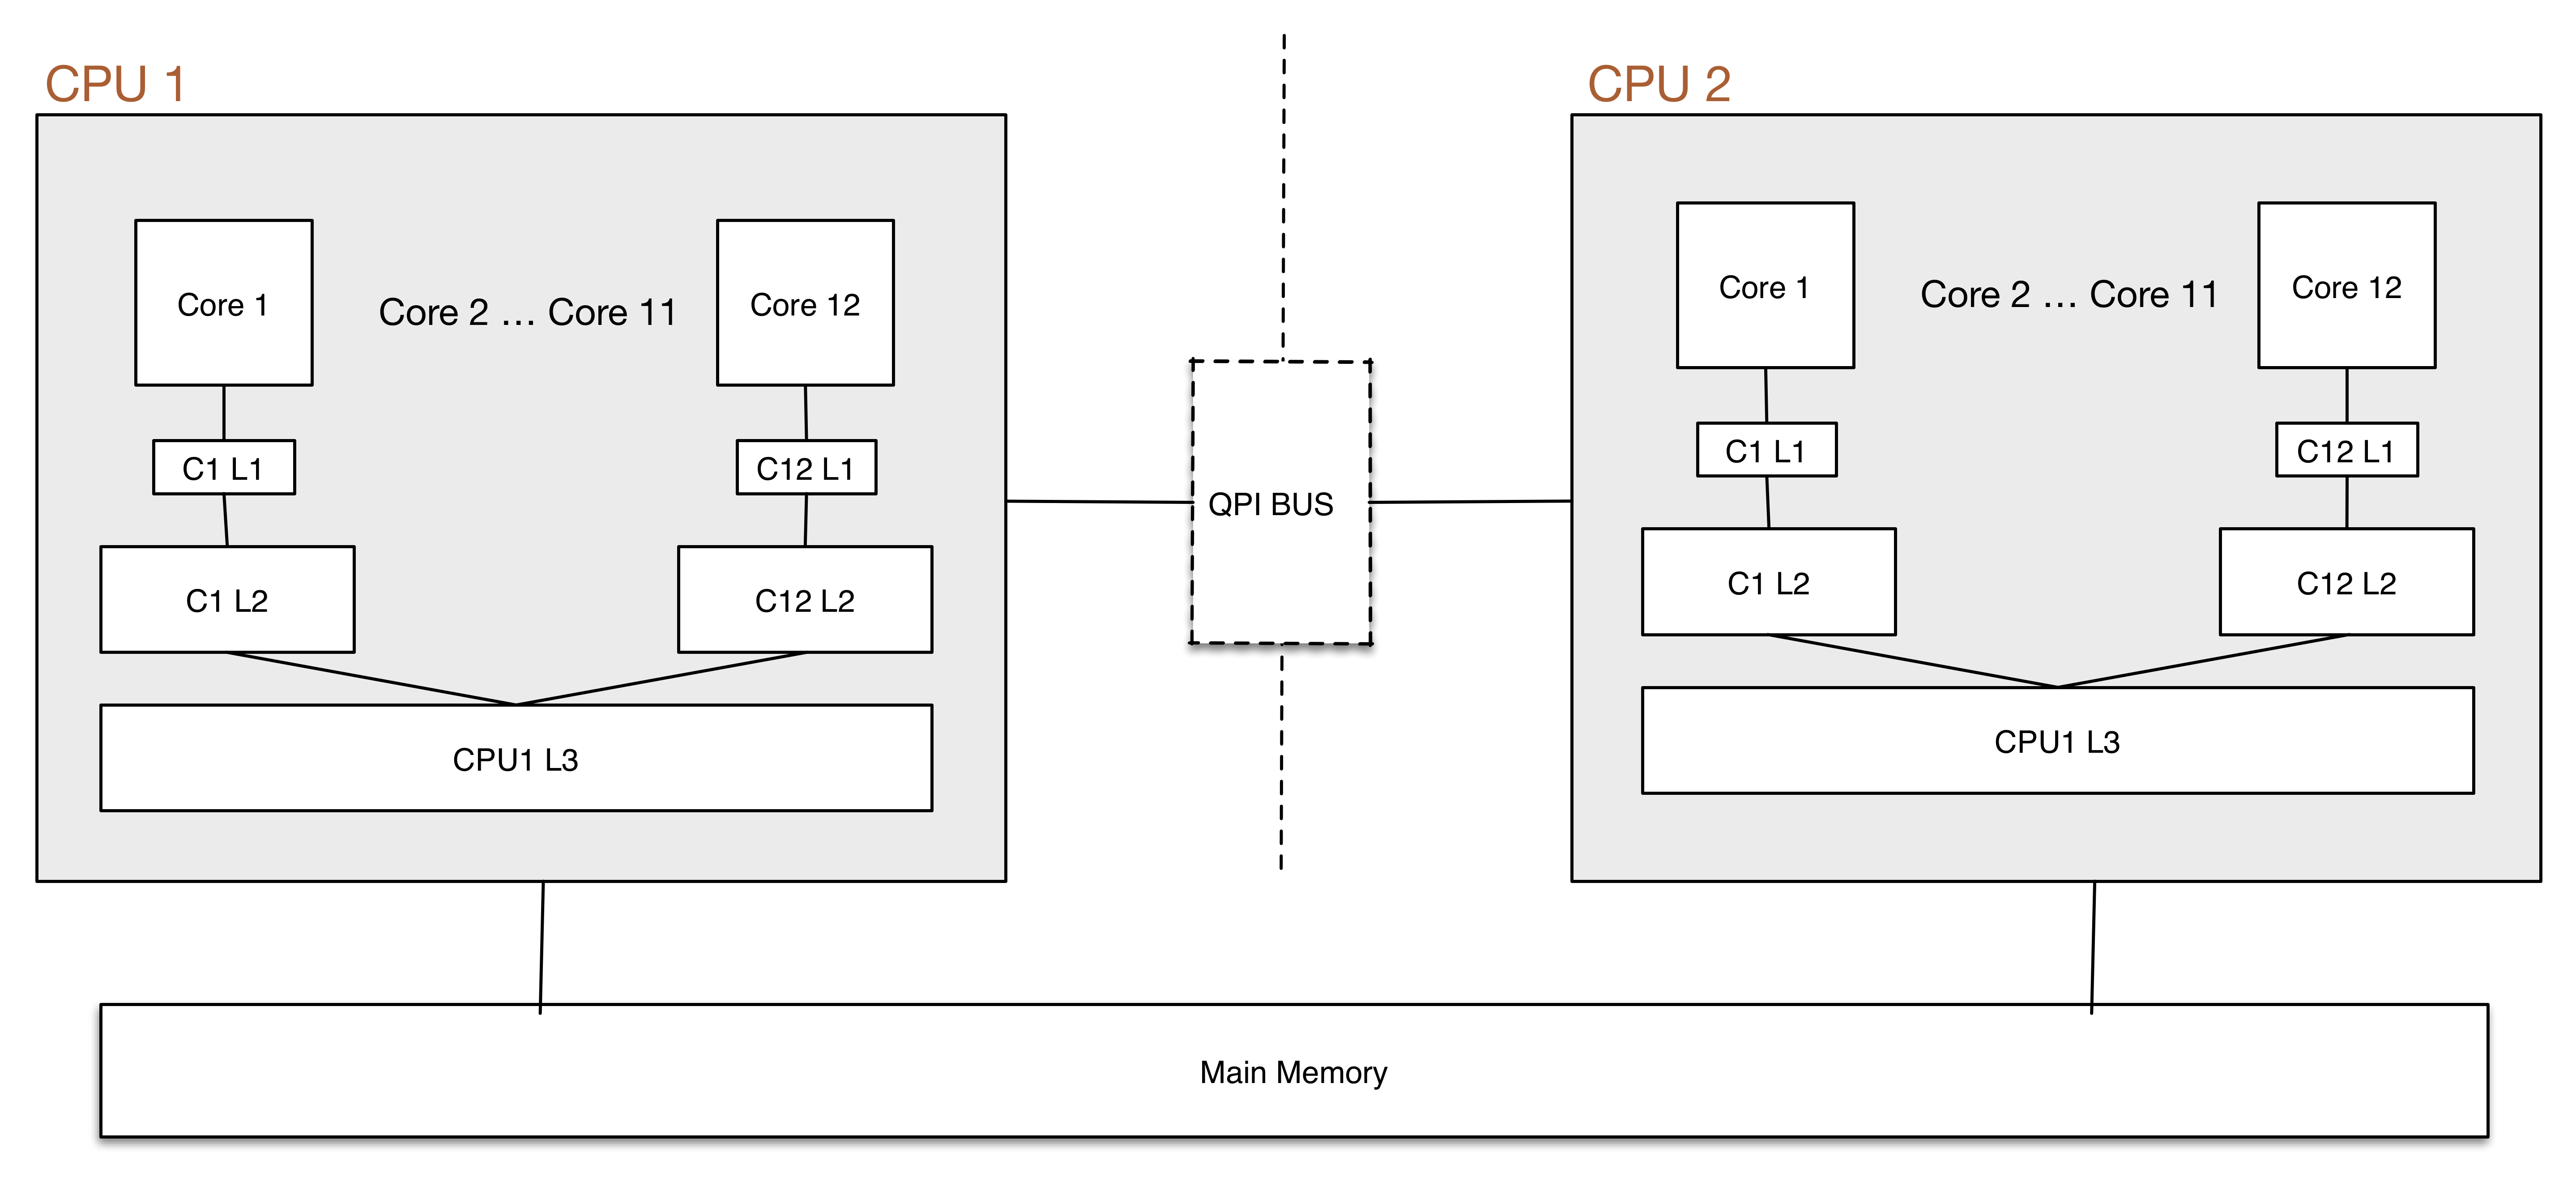
\includegraphics[width=145mm]{4/Xeon_E5-2695_v2.png}
\caption{Diagram of the layout of Xeon E5-2695 v2}
\label{layout_xeon_2695}
\end{figure}

The machine powered by Xeon 5130 consists of a single node, but the ICHEC's server is a workstation that consists of a number of units of computation. To be able to run the designed experiments, all tests had to be run on a single node. The experiments are relatively small, so any noticeable advantages could not be achieved by running experiments on multiple nodes. Both the Xeon 5130 and the Xeon E5-2695 v2 support the Intel® Hyper-Threading Technology (Intel® HT Technology) that allows an execution core to function as two logical processors. This technology was disabled on the Xeon 5130 to improve accuracy of achieved results. Disabling this feature could not be requested on the Xeon E5-2695 v2, although it is speculated that is is disabled by default.

\section{Constraints}
The designed experiments are constrained by a number of factors. Accuracy of results depends on isolation of processes/threads that belong to the run experiment and ability to terminate as many unnecessary processes as possible. Experiments are run from a Linux terminal, which allows to eliminate overhead caused by a GUI and other supporting system tasks, but the commands are executed with SSH that imposes additional overhead. The experiments are executed on hardware that was provided by the hosting university, access to more sophisticated and advanced machines could not be granted due to financial and bureaucratic reasons. All of these constraints were considered during the stage of designing the experimental environment and the experiments.

\section{Experiments}

A series of experiments were designed in the scope of the project. They are described in section \ref{experimentsDesign}. This section outlines how they can be run in the developed experimental environment and how results can be collected.

\subsection{Running Experiments on Servers}

All experiments were run from the terminal window on Mac OS X Mavericks. Both machines could be accessed by using the SSH protocol. Refer to figure \ref{terminal-nuim} for an image of the Terminal window with typed in commands that are required to SSH into the Xeon 5130, enter the directory with the source code of the experimental environment and the experiments, compile the code and run it. One may observe a \textit{make} command used to run the experiments. A makefile was created to optimise the process of running required experiments. Refer to appendix \ref{app:listingMakefile} for a source code of the file. This makefile can be used on both Linux-based Operating Systems and on Mac OS.

\begin{figure}[ht!]
\centering
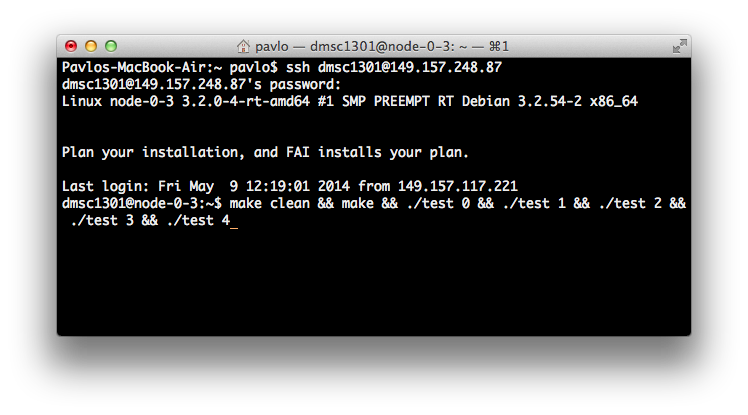
\includegraphics[width=145mm]{5/terminal-nuim.png}
\caption{Commands required to SSH into the Xeon 5130 and run the experiments}
\label{terminal-nuim}
\end{figure}

In case of the Xeon E5-2695 v2, since that machine has multiple nodes, the experiments had to be scheduled to be run on a single node. Refer to the Listing \ref{lst:ichecCommand} for the exact command used to schedule a job. This command was derived after reading documentation available at \cite{ICHEC2014a}. The \textit{qsub} command is utilised to explicitly send a job to a given queue. The argument \textit{-A nuim01} defines the account string associated with the job. Then, the argument \textit{-l nodes=1:ppn=24} specifies the resources that are required by the job, in this case one node and 24 units of computation associated with the node are asked. The \textit{walltime=0:29:00} mentiones the maximum amount of time that the job can be run for, in this case it says that the job can be run for the maximum of 29 minutes. Lastly, the argument \textit{-I} means that the new session needs to be interactive (with access to issuing new commands via the command prompt).
              
\begin{lstlisting}[
language=bash,
caption={Command to schedule a job on one node in the Xeon E5-2695 v2},
label={lst:ichecCommand}
]
qsub -A nuim01 -l nodes=1:ppn=24 walltime=0:29:00 -I
\end{lstlisting}

Files with source code can be copied onto the servers and back by the secure copy command \textit{scp}. Measured data can then be analysed on the local machine.

\subsection{Execution of Experiments}

When the experimental environment is compiled, the experiments are ready to be run. All experiments could be executing by running the compiled experimental environment and passing a single argument: a ID of an experiment. For example, a command \textit{./test 2} will run the Experiment 2. When experiments are executed, different information may be outputted. A level of details in the information shown to a user may be configured by defining variables \textit{DEBUG} and \textit{DETAILED\_DEBUG} (by default defined in the \textit{conf.h}\footnote{\url{https://github.com/Hollgam/Impact-of-cache-on-multi-threaded-programmes/blob/master/test/
src/conf.h}} file). If a variable \textit{SHOW\_RESULTS} is defined, the summary of results from running the experiments is also outputted onto the screen. 

To continue, the experimental environment could not be prepared to support completely free from the impact of the Operating System experiments. It was decided to produce two CSV files for each experiment. One file with filtered data and another one with unfiltered data. Files are named as \textit{``CPU\_TYPE-EXPERIMENT-RUN.csv"}, where \textit{CPU} indicates a type of CPU that an experiment was run on (e.g. ``xeon"), \textit{TYPE} shows the type of data stored in the file (can be either ``clean" for filtered data or ``dirty" for unfiltered data), \textit{EXPERIMENT} gives the ID of the experiment, and \textit{RUN} shows a run of the experiment (if an experiment is run more than once, individual CSV files are generated for each run). All files are placed in a \textit{results} folder. They present quantitative information gathered before and after running experiments and mention numbers of any interrupts and minor and major page faults detected while executing the experiments. Files with filtered data contain timing results only from running those experiments that were not interrupted by interrupts or page faults, i.e. if such unwanted processes were detected during execution of all runs of an experiment, its duration is noted as ``0".

\begin{table*}
\caption{A sample of a CSV file with filtered data}
\centering 
\scalebox{0.8}{
    \begin{tabular}{lllllllllll}
    N         & Time   & TimeMin   & 1.INT & 1.PFMIN & 1.PFMAJ & 2.INT & ... & 10.INT & 10.PFMIN & 10.PFMAJ \\
    0         & 581742 & 581742 & 0     & 6       & 0       & 0     & ... & 0      & 2        & 0        \\
    8         & 591849 & 581742 & 0     & 0       & 0       & 0     & ... & 0      & 2        & 0        \\
    16        & 583742 & 581742 & 0     & 0       & 0       & 0     & ... & 0      & 2        & 0        \\
    ...       & ...    & ... & ...   & ...     & ...     & ...   & ... & ...    & ...      & ...      \\
    128000064 & 0      & 581742 & 38    & 31253   & 0       & 38    & ... & 37     & 31253    & 0        
    \end{tabular}
}
\label{csvTable}
\end{table*}

Refer to table \ref{csvTable} for a sample of a file that contains filtered data for an experiment that was run for a selection of data exchanged between two threads, starting from 0 bytes (for calculating overhead imposed by the OS) and finishing with 128000064 bytes of data exchanged between two threads (shown in a column \textit{N}). Each test in the experiment is run ten times. The duration presented in the second column \textit{Time} is an average of duration of each of ten tests. If reported in the file data is filtered, only those tests that qualify for being ``uninterrupted" are taken into account. Information about recorded interrupts, minor page faults, and major page faults is recorded for each sub-experiment (run with a specific value given to the parameter -- the amount of exchanged data) of the experiment in columns (\textit{N.INT}, \textit{N.PFMIN}, and \textit{N.PFMAJ} respectively, where \textit{N} indicates an ID of the test). It could be observed that tests are affected from overhead of the OS. If one looked at the last row in the sample, it is apparent that tests with a large amount of data exchanged between threads (in this case 128 MB) do indeed suffer from large numbers of interrupts and minor page faults.

\subsection{Cycle-Level Experiments. Experiments 0 and 1}
\label{conducting_cycle}

Experiment 0 and Experiment 1 were executed to provide cycle-level measurements. The \textit{RDTSC} instruction was used to measure time because, as was shown in \ref{measuringTime}, it is more reliable than \textit{clock\_gettime(3)}. However, received results are unrealistic and unsatisfactory. It may be speculated that due to the thread scheduling performed by the Operating System, the \textit{RDTSC} instruction is executed out of order, before entering the loop where data is written and read (refer to listings \ref{listingExperiment0} and \ref{listingExperiment1}). Usage of \textit{clock\_gettime(3)} resulted in the same behaviour.

Almost no differences in data marked as filtered and unfiltered could be found, all measurements were obscured by the overhead caused by the OS. Hence it was accepted that no accurate data can be collected by running the designed cycle-level experiments. A decision was made to use one of the benchmarks described in section \ref{sec:benchmarks}. After evaluating all tools listed in that section and their applicability to measuring latency in the given laboratory environment, lmbench \cite{McVoy2012} was chosen as the most suitable suite. Running experiments with this benchmark is a complicated undertaking. The benchmark has not been updated since the end of 1990's and little documentation is available. It is an open-source product that used to be supported by Intel, but the source code is difficult to interpret.

One of the benchmarks available in the lmbench suite \textit{lat\_mem\_rd}\footnote{\url{http://www.bitmover.com/lmbench/lat_mem_rd.8.html}} was utilised as a tool for measuring latency of memory and cache \cite{Ruggiero2008}. The instructions that were given in \cite{Ruggiero2008} did not work on the servers used for running experiments as no output could be gathered due to unknown reason. An attempt was made to run the full benchmark on the Xeon 5130. It tests all aspects of the system. The problem with the tool is that it asks a number of questions about hardware and some of them could not be answered with full certainty, since information that would allow to provide answers could not be accessed. A number of educated guesses were taken and a summary of results was received.  

Working with the tool on the Xeon E5-2695 v2 was much more complicated. Because of the set-up used in the Xeon E5-2695 v2, it is not possible to run interactive sessions for more than 29 minutes. As a results, no summary of results could be received, as it is outputted on the screen. A alternative was found: a bash script was written that allows to redirect output into a textual file and send a summary via email. Refer to the Appendix \ref{app:listingLmbenchICHEC} for the source code of the script. A large number of attempts to configure it and make the benchmark run successfully had to be taken. Because of different reasons the job would be terminated before it can finish its execution. Refer to listing \ref{listingJobError} for an example of an error message that would be returned after the termination of the script, in this case the job could not be finished because it timed out. Due to an unknown problem, a few times the job also terminated from occurrence of a segmentation fault. In an attempt to overflow the allowed hard disk space, it would cause a core dump. Examination of the source code of the benchmark did not lead into finding the reason for such problem.

\begin{lstlisting}[
language=C,
caption={The error message caused by termination of lmbench on the Xeon E5-2695 v2},
label={listingJobError}
]
PBS Job Id: 174345.service1.cb3.ichec.ie
Job Name:   lmbench
Exec host: r1i7n3/0+r1i7n3/1+r1i7n3/2+r1i7n3/3+r1i7n3/4+r1i7n3
/5+r1i7n3/6+r1i7n3/7+r1i7n3/8+r1i7n3/9+r1i7n3/10+r1i7n3/11+r1i
7n3/12+r1i7n3/13+r1i7n3/14+r1i7n3/15+r1i7n3/16+r1i7n3/17+r1i7n
3/18+r1i7n3/19+r1i7n3/20+r1i7n3/21+r1i7n3/22+r1i7n3/23
Aborted by PBS Server 
Job exceeded its walltime limit. Job was aborted
See Administrator for help
Exit_status=-11
resources_used.cput=04:59:34
resources_used.mem=46238200kb
resources_used.vmem=46363608kb
resources_used.walltime=05:00:36
\end{lstlisting}

However, certain data could be measured. Lmbench runs tests on memory by varying its stride. Examining the source code revealed that the benchmark controls two nested for-loops. The outer loop changes the stride size, the inner loop varies the array size. For each array size, the benchmark creates a ring of pointers that point forward one stride. Nevertheless, information about memory latency for different values of the \textit{stride} parameter could not be extracted due to time limitations and lack of support from creators of lmbench. Much later, close to the end of the project, an undocumented and unlisted script \textit{cache} was found in the distribution of lmbench. That application was then used to receive information about latency of cache and main memory.
   
\subsection{Application-Level Experiments. Experiments 2 -- 4}

Running application-level experiments was less complicated and more straight-forward than execution of the cycle-level experiments. For measuring duration of the application-level experiments \textit{clock\_gettime(3)} was used because it outputs information about the system-wide clock, and not the data that is dependant on CPU cores. Even though it is less stable than the \textit{RDTSC} instruction (which is core-dependant), the accuracy of the tool used for timing is not crucial on the application level. All experiments also produced both filtered and unfiltered data.

% ---------------------------------------------------------------------------
%: ----------------------- end of thesis sub-document ------------------------
% ---------------------------------------------------------------------------


% this file is called up by thesis.tex
% content in this file will be fed into the main document

%: ----------------------- name of chapter  -------------------------
\chapter{Results} % top level followed by section, subsection
\label{resultsChapter}

This chapter introduces results that were measured from all five programmes, both cycle- and application-level experiments. All reported results are based on ten runs for all buffer sizes. There are multiple figures in the chapter, some of them cannot be rendered on the pages where they are referenced due to their large sizes.

%: ----------------------- paths to graphics ------------------------

% change according to folder and file names
\ifpdf
    \graphicspath{{X/figures/PNG/}{X/figures/PDF/}{X/figures/}}
\else
    \graphicspath{{X/figures/EPS/}{X/figures/}}
\fi

%: ----------------------- contents from here ------------------------

\section{Cycle-Level Experiments}

\label{sec:cycle_results}

\subsection{Experiment 0}

As identified in section \ref{design_env}, it was learnt through running experiments that a number of page faults cannot be avoided for even the shortest experiments. Gathering results that are not affected by the processes that take place in the OS proved to be impossible in the given environment. The act of reading the interrupts count generates page faults. The base Experiment 0 showed that on average accessing data from a CPU register takes 349 clock-cycles.

\subsection{Experiment 1}

Refer to figures \ref{Cycle_experiment_clean_nuim} and \ref{Cycle_experiment_dirty_nuim} for the graphs where unfiltered and filtered (respectively) data measured by running Experiment 1 on the Xeon 5130 is plotted. Filtered data indicates results that are not affected by overhead of the OS; unfiltered data reports measurements as they are seen in the environment, including overhead. On these graphs the x-axes represent the numbers of bytes transferred using the array \textit{testAr}. Data is written/read in a form of \textit{long} words, which are 8 bytes each, on both systems used in the project. The value is defined by the argument \textit{n} that is passed to the experiment function. The y-axes plot how much time (measured in clock-cycles) it takes to write \textit{n} bytes into memory and subsequently read them from memory. Detailed filtered results of first three runs of all iterations of the experiment with an indication of the numbers of interrupts and minor page faults that were recorded while running the experiment in this setting may be found in appendix \ref{app:cycle-level-results-clean-nuim}.

\begin{figure}[!htb]
\centering
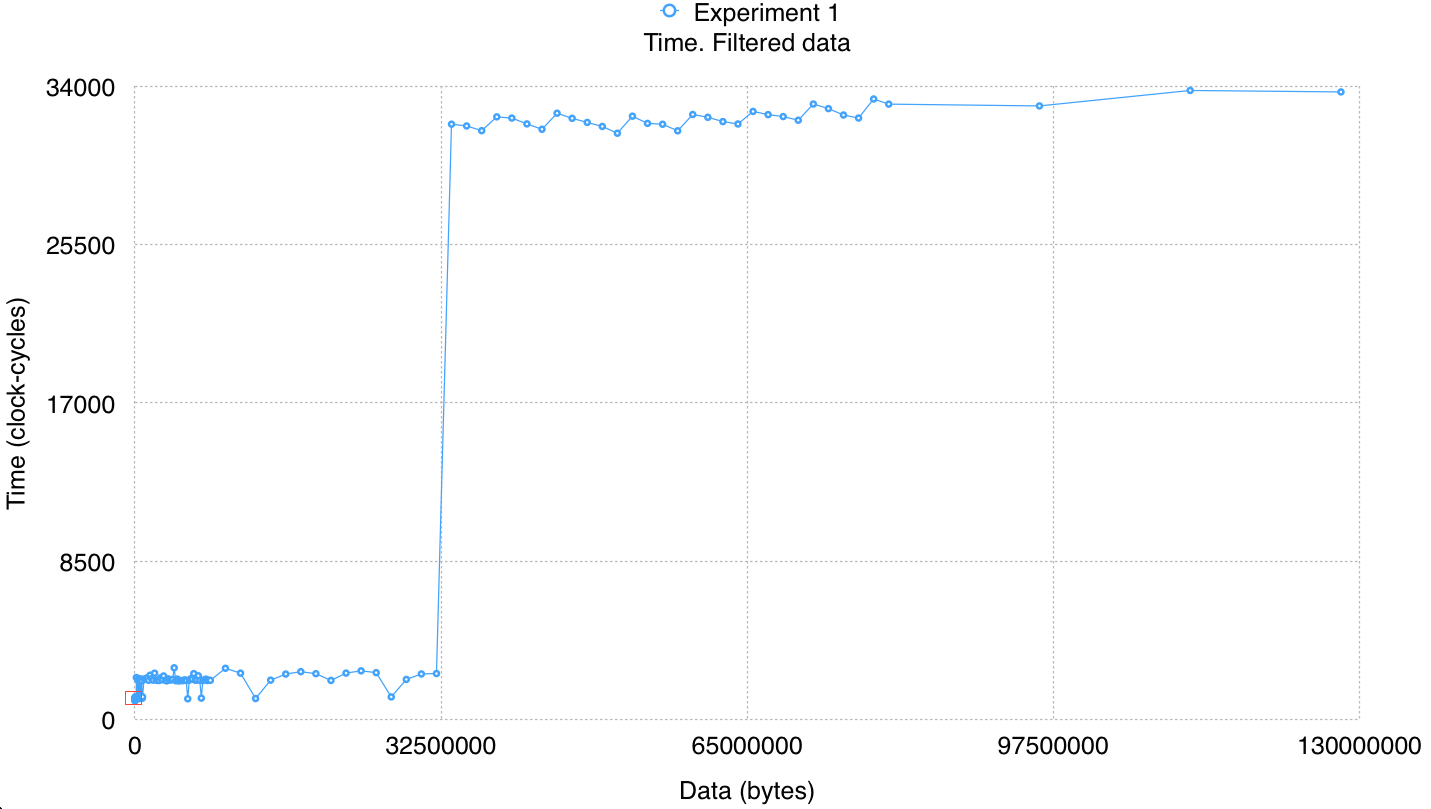
\includegraphics[width=145mm]{6/Cycle_experiment_clean_nuim.png}
\caption{Xeon 5130: data copying times (filtered data, Experiment 1)}
\label{Cycle_experiment_clean_nuim}
\end{figure}

\begin{figure}[!htb]
\centering
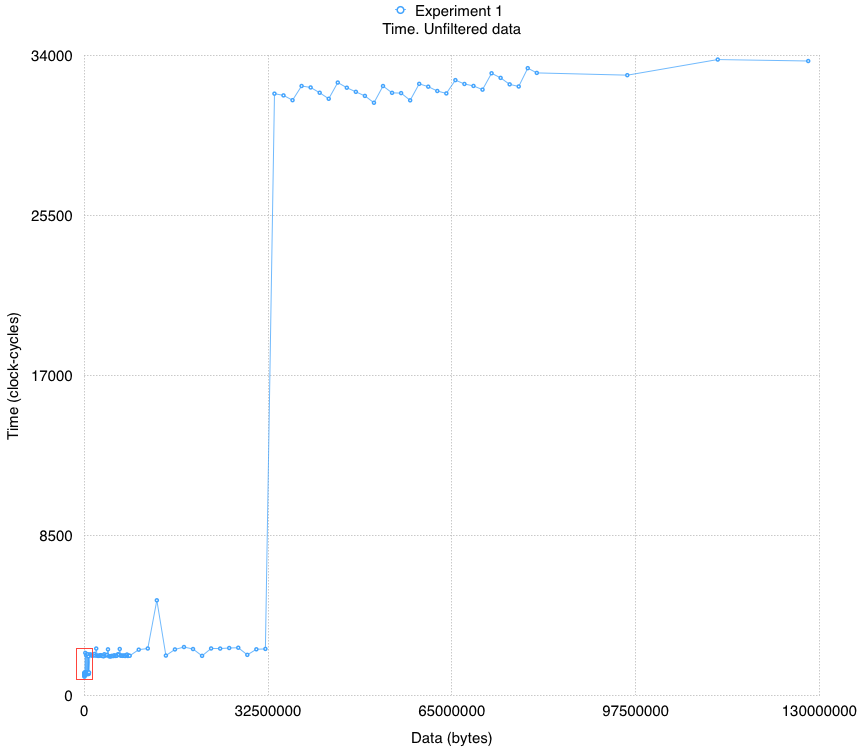
\includegraphics[width=145mm]{6/Cycle_experiment_dirty_nuim.png}
\caption{Xeon 5130: data copying times (unfiltered data, Experiment 1)}
\label{Cycle_experiment_dirty_nuim}
\end{figure}

Figures \ref{Cycle_experiment_clean_nuim_small} and \ref{Cycle_experiment_dirty_nuim_small} are similar to graphs \ref{Cycle_experiment_clean_nuim} and \ref{Cycle_experiment_dirty_nuim}. They also plot filtered and unfiltered data (respectively) measured from running Experiment 1 on the Xeon 5130, but they focus on the results of running the experiment with $8 <= n <= 400064$. The relative parts of the graphs, which are ``zoomed in" are outlined by red rectangles on the figure \ref{Cycle_experiment_clean_nuim} and \ref{Cycle_experiment_dirty_nuim}.

\begin{figure}[!htb]
\centering
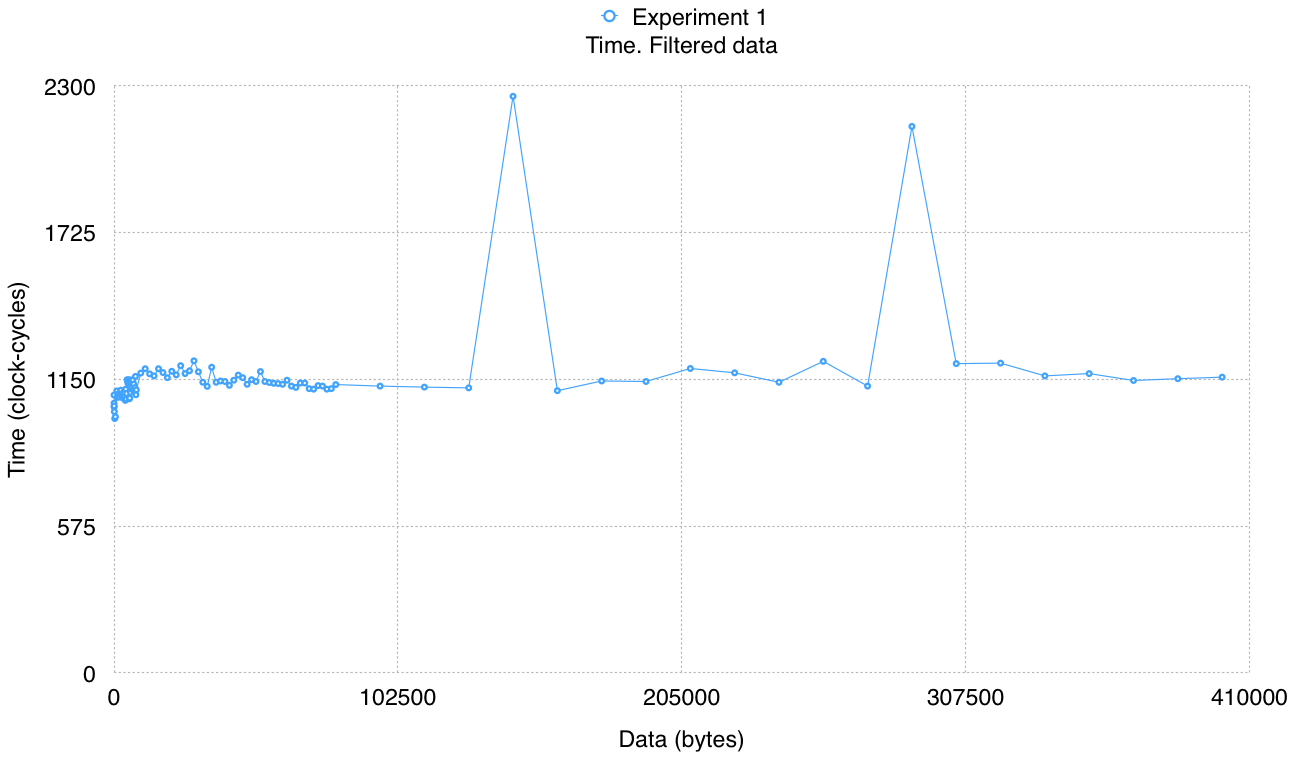
\includegraphics[width=145mm]{6/Cycle_experiment_clean_nuim_small.png}
\caption{Xeon 5130: data copying times, where $8 <= n <= 400064$ (filtered data, Experiment 1)}
\label{Cycle_experiment_clean_nuim_small}
\end{figure}

\begin{figure}[!htb]
\centering
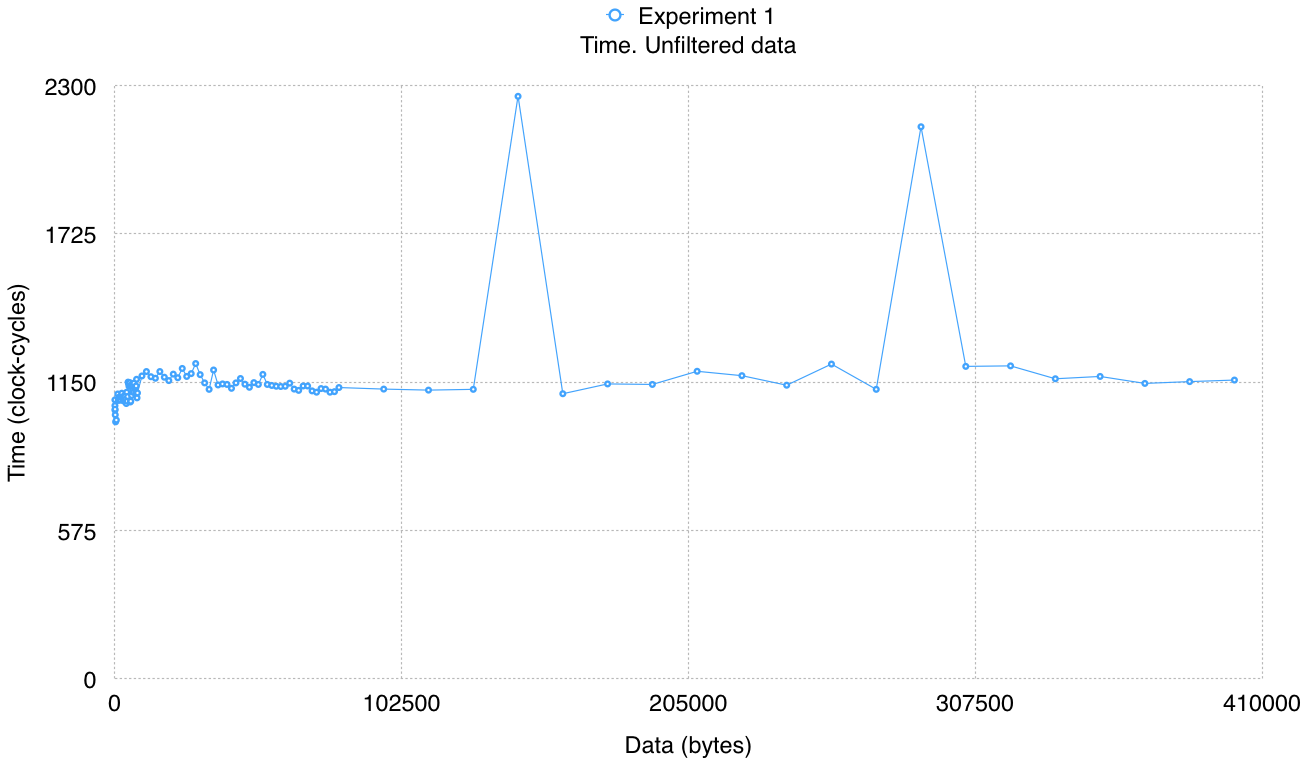
\includegraphics[width=145mm]{6/Cycle_experiment_dirty_nuim_small.png}
\caption{Xeon 5130: data copying times, where $8<= n <= 400064$ (unfiltered data, Experiment 1)}
\label{Cycle_experiment_dirty_nuim_small}
\end{figure}

Refer to figures \ref{Cycle_experiment_clean_ichec} and \ref{Cycle_experiment_dirty_ichec} for the graphs where unfiltered and filtered (respectively) data measured by running Experiment 1 on the Xeon E5-2695 v2 is plotted. As in the case of graphs showing results of running this experiment on a different machine, in these graphs the x-axes represent numbers of bytes written into the array \textit{testAr}. The value is defined by the argument \textit{n} that is passed to the experiment function. The y-axes plot how much time (measured in clock-cycles) it takes to write \textit{n} bytes into memory and subsequently read them from memory. Again, detailed filtered results of first three runs of all iterations of the experiment with an indication of the numbers of interrupts and minor page faults that were recorded while running the experiment in this setting may be found in appendix \ref{app:cycle-level-results-clean-ichec}.

\begin{figure}[!htb]
\centering
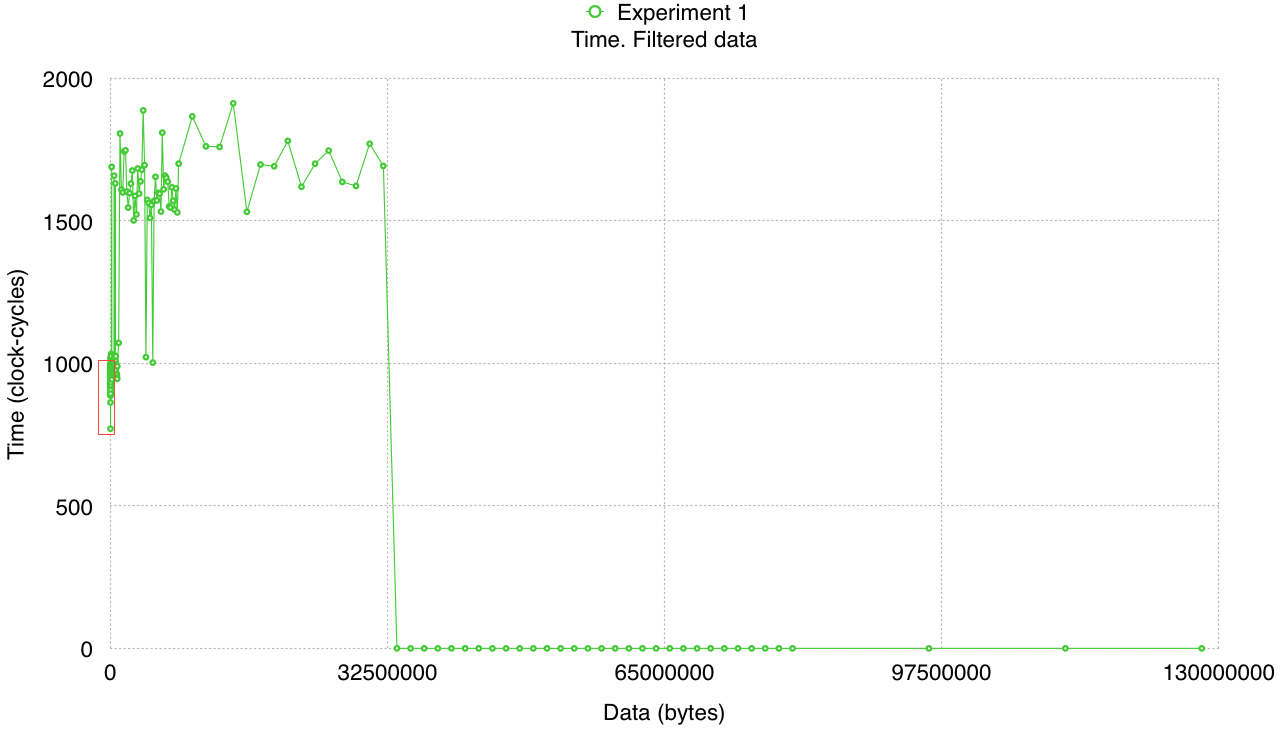
\includegraphics[width=145mm]{6/Cycle_experiment_clean_ichec.png}
\caption{Xeon E5-2695 v2: data copying times (filtered data, Experiment 1)}
\label{Cycle_experiment_clean_ichec}
\end{figure}

Data that was measured on the Xeon E5-2695 v2 was especially ``noisy". It may be caused by the fact that, compared to the Xeon 5130, it is a much more complicated machine where many more processes take place. For $n >= 33600064$, the amount of interrupts and minor page faults generated in the system was so large (at least 4 minor page faults in each run) that all runs of the experiment were seen as ``overly-noisy" data and could not filtered, i.e. all of them are marked as having $t = 0$, where $t$ is execution time.

\begin{figure}[!htb]
\centering
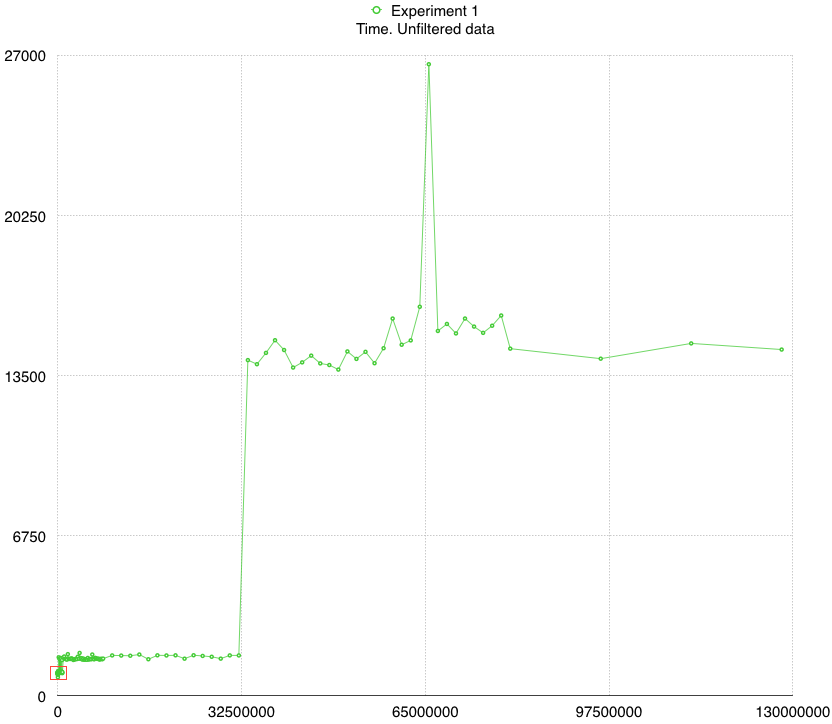
\includegraphics[width=145mm]{6/Cycle_experiment_dirty_ichec.png}
\caption{Xeon E5-2695 v2: data copying times (unfiltered data, Experiment 1)}
\label{Cycle_experiment_dirty_ichec}
\end{figure}

Figures \ref{Cycle_experiment_clean_ichec_small} and \ref{Cycle_experiment_dirty_ichec_small} are similar to graphs \ref{Cycle_experiment_clean_ichec} and \ref{Cycle_experiment_dirty_ichec}. They plot filtered and unfiltered data (respectively) measured from running Experiment 1 on the Xeon E5-2695 v2, but they focus on the results of running the experiment with $8 <= n <= 400064$. The relative parts of the graphs, which are ``zoomed in" are outlined by red rectangles on the figure \ref{Cycle_experiment_clean_ichec} and \ref{Cycle_experiment_dirty_ichec}.

\begin{figure}[!htb]
\centering
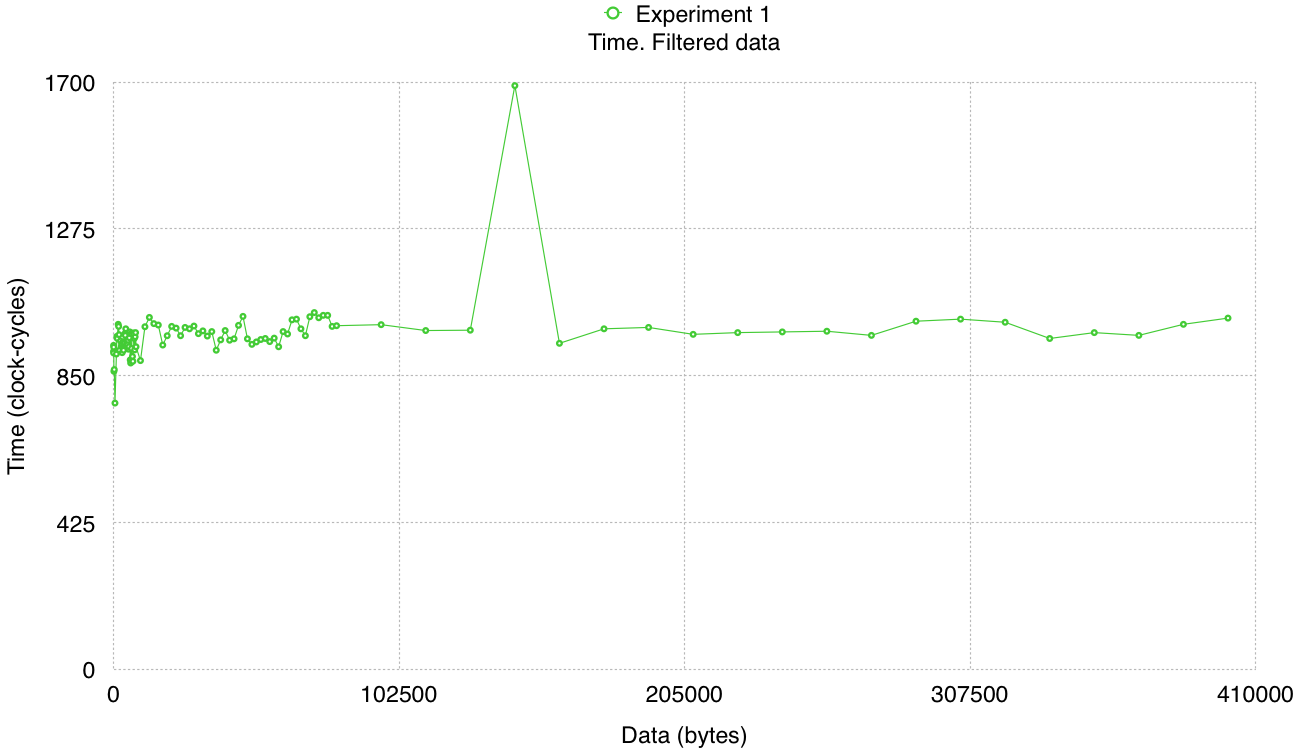
\includegraphics[width=145mm]{6/Cycle_experiment_clean_ichec_small.png}
\caption{Xeon E5-2695 v2: data copying times, where $8 <= n <= 400064$ (filtered data, Experiment 1)}
\label{Cycle_experiment_clean_ichec_small}
\end{figure}

\begin{figure}[!htb]
\centering
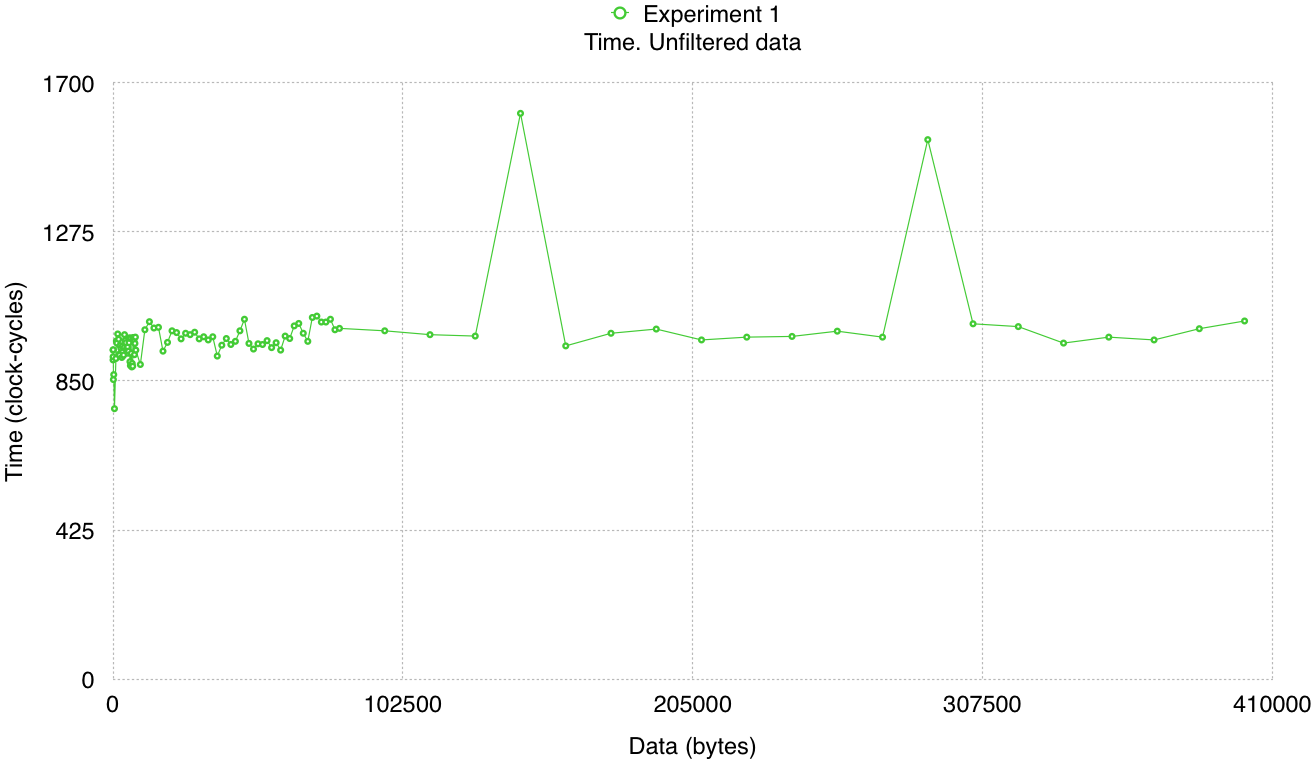
\includegraphics[width=145mm]{6/Cycle_experiment_dirty_ichec_small.png}
\caption{Xeon E5-2695 v2: data copying times, where $8 <= n <= 400064$ (unfiltered data, Experiment 1)}
\label{Cycle_experiment_dirty_ichec_small}
\end{figure}

A couple of ``big spikes" and a number of ``smaller spikes" may be seen on all graphs described in this section \ref{sec:cycle_results}, these abnormalities may be explained by the occurrence of interrupts and page faults that could not be filtered out, i.e. they were not only caused by the only unavoidable process that could be proven as such that generated minor page faults – opening files – and thus were caused by other processes run by the OS. On a smaller scale, where a small amount of data is shared between threads ($< 1000$ bytes), such behaviour may be explained by the fact that data is fetched from cache in pieces of information that are dividable by the size of a cache line. Also, one may argue that because it was not clear if hyper-threading is disabled on the Xeon E5-2695 v2, it may have had an impact as well. The experiments were run multiple times, but each time such abnormalities could not be isolated out.

In the end, the testing environment could not be configured to remove all overhead caused by the Operating System and all other processes that are executed when cycle-level experiments are run. Information on latency of cache and main memory was measured with lmbench, as described in the following section.

\subsection{Measuring Latency of Cache with lmbench}
\label{results_lmbench}

The lmbench tool reports that the Xeon 5130 machine has 0.5 ns timer accuracy and the Xeon E5-2695 v2 has 0.25 ns timer accuracy. Together with the chief technician of the faculty the author examined the source code of lmbench, which allowed to evaluate methods that are used in the benchmark. This evaluation revealed that it was not possible to configure the way the programme chooses its stride for ``jumping" between data samples. The stride value is important as it allows to configure the size of the buffer that is used in the benchmark; a correct value of this parameter will make sure that no levels of memory can be ``jumped over".

Figure \ref{lmbench_nuim} shows results of running \textit{lat\_mem\_rd} on the Xeon 5130. The x-axis represents the amount of data that is written into memory, the y-axis shows how many nano-seconds writing that data into memory takes. This plot shows how latency increases when the amount of data written into memory approaches the size of Level 2 cache, when data has to be written into main memory (more data is exchanged between threads that can fit into cache), the graph starts to flatten out.

\begin{figure}[!htb]
\centering
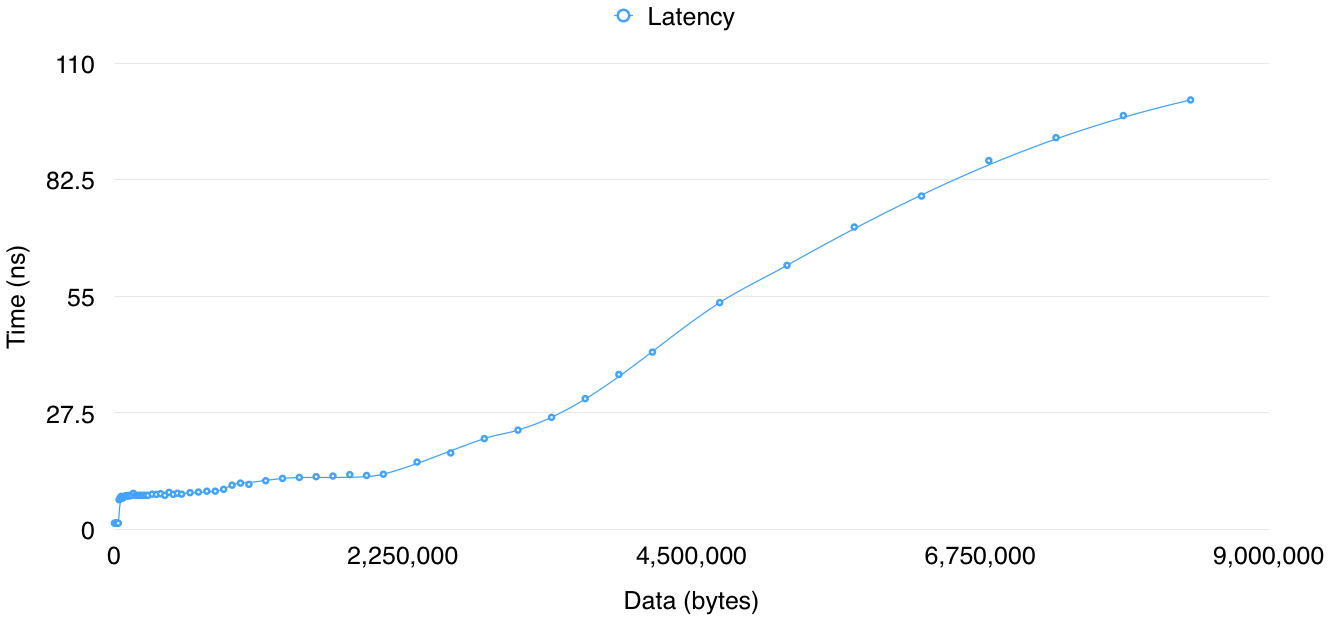
\includegraphics[width=145mm]{6/lmbench_nuim.png}
\caption{Xeon 5130: latency of cache, measured with lmbench}
\label{lmbench_nuim}
\end{figure}

Figure \ref{lmbench_ichec} shows results of running \textit{lat\_mem\_rd} on the Xeon E5-2695 v2. Similar to the figure \ref{lmbench_nuim}, the x-axis represents the amount of data that is written into memory, the y-axis shows how many nano-seconds writing that data into memory takes. Similar to figure \ref{lmbench_nuim}, one can see a ``jump" when the amount of data exchanged between threads approaches the size of Level 3 cache, then it gradually flattens out, as data is written into main memory at that stage. 

\begin{figure}[!htb]
\centering
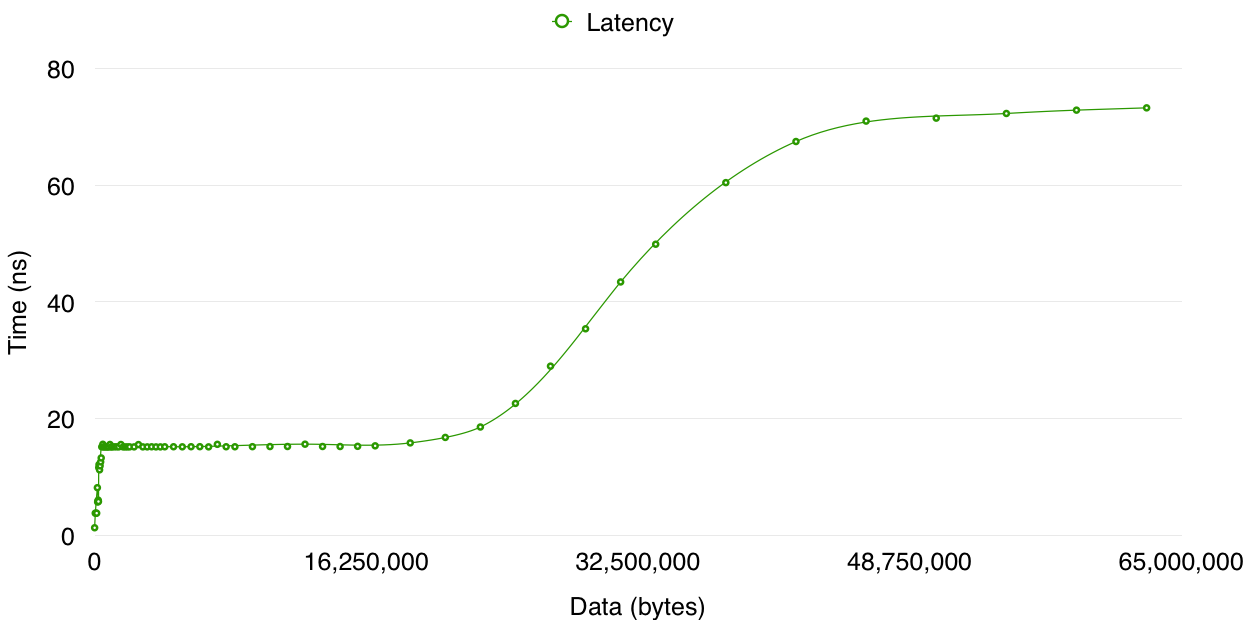
\includegraphics[width=145mm]{6/lmbench_ichec.png}
\caption{Xeon E5-2695 v2: latency of cache, measured with lmbench}
\label{lmbench_ichec}
\end{figure}

As was described in section \ref{conducting_cycle}, lmbench was difficult to operate. Mixed results were received. However, when the \textit{./cache} application was discovered, it became possible to verify assumptions made by running the \textit{lat\_mem\_rd} benchmark. Refer to table \ref{lmbenchTable} for results received from executing the \textit{./cache} programme. Close examination of the figures \ref{lmbench_nuim} and \ref{lmbench_ichec} and data presented in Appendix \ref{app:lmbench-results} shows that both benchmarks indicate the same values of latency of cache and memory. One may notice ``jumps" when the sizes of levels of cache are reached on the graphs.

\begin{table*}
\caption{Latency of cache and main memory as reported by lmbench}
\centering 
\begin{tabular}{lllll}
             & L1 cache & L2 cache & L3 cache & Main memory \\
Xeon 5130  & 1.5      & 7.0      & None     & 100.0         \\
Xeon E5-2695 v2 & 1.25     & 3.75     & 15.5     & 60.0       
\end{tabular}
\label{lmbenchTable}
\end{table*}

Results achieved by executing cycle-level experiments allowed to derive values of latency in two distinctly-different environments that are used in chapter \ref{discussionChapter} to discuss the model presented in chapter \ref{chapterModel}.

\section{Application-Level Experiments. Experiments 2 -- 4}
\label{results_app_experiments}

Figures \ref{App_experiment_1_throughput_dirty_nuim} and \ref{App_experiment_1_throughput_dirty_ichec} show unfiltered data measured through running three application-level experiments on the Xeon 5130 and the Xeon E5-2695 v2. In both cases, the x-axis represents the amount of data that is exchanged between threads, the y-axis shows the throughput ($n / t$, where $n$ indicated the amount of data exchanged between threads and $t$ represents the amount of time spent of exchanging the data).

\begin{figure}[!htb]
\centering
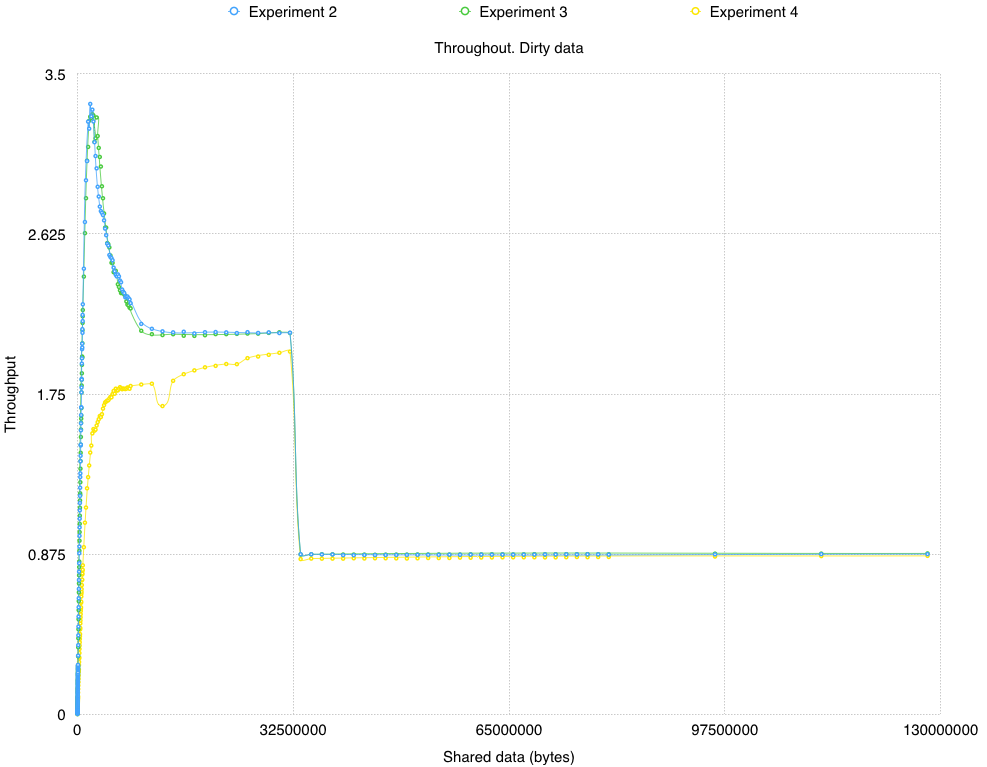
\includegraphics[width=145mm]{6/App_experiment_1_dirty_throughput_nuim.png}
\caption{Xeon 5130: throughput of copying data in inter-thread communication (Experiments 2-4)}
\label{App_experiment_1_throughput_dirty_nuim}
\end{figure}

\begin{figure}[!htb]
\centering
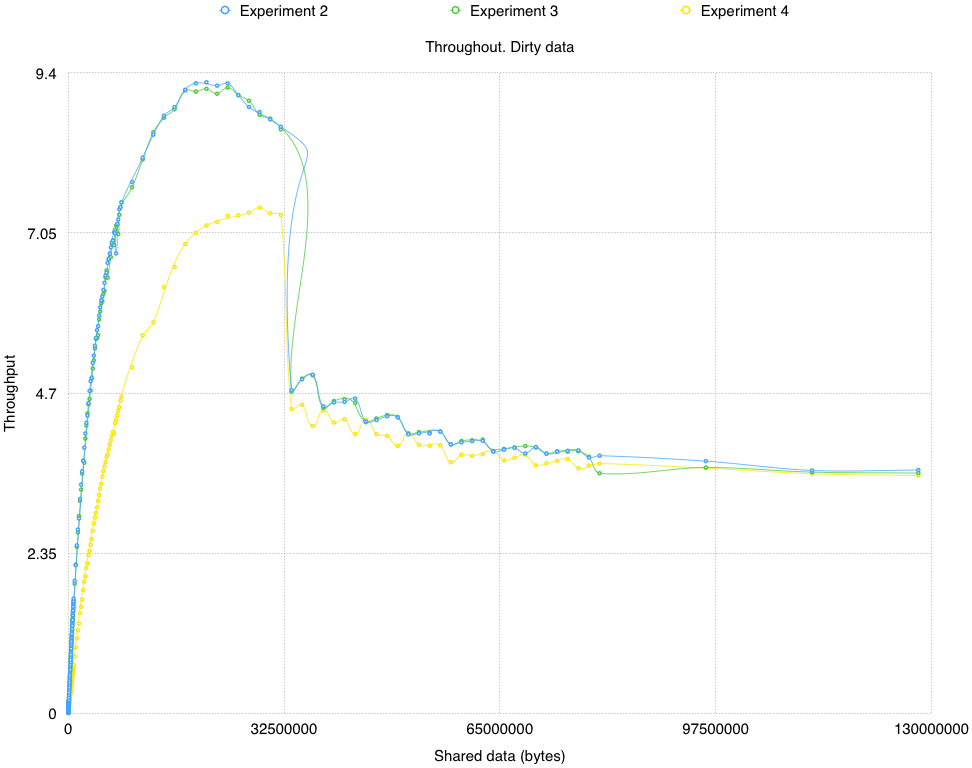
\includegraphics[width=145mm]{6/App_experiment_1_dirty_throughput_ichec.png}
\caption{Xeon E5-2695 v2: throughput of copying data in inter-thread communication (Experiments 2-4)}
\label{App_experiment_1_throughput_dirty_ichec}
\end{figure}

Both graphs exhibit decrease of throughput when the amount of shared between threads data exceeds 33600064 bytes (32.0435 MB). The fact that such behaviour was observed and on both systems with different architectures was not anticipated. The graph \ref{App_experiment_1_throughput_dirty_ichec} also shows ``waves" after reaching the 32.0435 MB mark. It is expected that all data larger than the size of Level 3 cache (30 MB) should be placed in the main memory, provided that it is smaller than the size of main memory. Therefore, no fluctuations could be expected.

As with results achieved by running the cycle-level experiments, detailed unfiltered results of first three runs of all iterations of the experiments with an indication of the numbers of interrupts and minor page faults that were recorded while running the experiments may be found in the following appendices:

\begin{itemize}
  \item Experiment 2 executed on the Xeon 5130: appendix \ref{app:app-level-results-2-nuim};
  \item Experiment 2 executed on the Xeon E5-2695 v2: appendix \ref{app:app-level-results-2-ichec};
  \item Experiment 3 executed on the Xeon 5130: appendix \ref{app:app-level-results-3-nuim};
  \item Experiment 3 executed on the Xeon E5-2695 v2: appendix \ref{app:app-level-results-3-ichec};
  \item Experiment 4 executed on the Xeon 5130: appendix \ref{app:app-level-results-4-nuim};
  \item Experiment 4 executed on the Xeon E5-2695 v2: appendix \ref{app:app-level-results-4-ichec}.
\end{itemize}

% \begin{figure}[!htb]
% \centering
% \includegraphics[width=145mm]{6/App_experiment_1_dirty_time_nuim.png}
% \caption{Results from the application-level experiment (time, unfiltered data). On the Xeon 5130. \hl{PLOT IN R}}
% \label{App_experiment_1_time_dirty_nuim}
% \end{figure}

% \begin{figure}[!htb]
% \centering
% \includegraphics[width=145mm]{6/App_experiment_1_dirty_time_ichec.png}
% \caption{Results from the application-level experiment (time, unfiltered data). On the Xeon E5-2695 v2. \hl{PLOT IN R}}
% \label{App_experiment_1_time_dirty_ichec}
% \end{figure}

Similar to the cycle-level experiments, running the application-level experiments within the experimental environment built for this project could not be configured in a way that would allow to receive accurate and fully-filtered data. Nevertheless, due to the nature of the application-level experiments that were run in the scope of this research, timing results that together with duration of the actual experiments also incorporate overhead caused by the operating system, may also be seen as satisfactory. More specifically, page faults, interrupts and other unwanted processes take considerably less time than the actual tests. Filtered data may be ignored as it was impossible to find a way to control the overhead imposed by the OS.

Finally, the overhead of the Operating System was measured for all three cases of inter-thread communication (described in Section \ref{taxonomy}). Such measurement was done by executing experiments with no data exchanged between two threads, i.e. only overhead of creating threads, creating a mutex, joining threads, and freeing memory was recorded. Each experiment was performed 1000 times and standard deviation (SD) was also calculated. Table \ref{overheadTable} gives a summary of the amount of overhead and its standard deviation (in nano-seconds) of performing the aforementioned operations. The standard deviation in all cases is not large: 1 -- 4\%.

\begin{table*}
\caption{Overhead of inter-thread communication}
\centering 
\begin{tabular}{llll}
             & Experiment 2 & Experiment 3 & Experiment 4 \\
Xeon 5130 (overhead) & 291408       & 297691       & 699229       \\
Xeon 5130 (SD) & 6320      & 5095       & 11694      \\
Xeon E5-2695 v2 (overhead) & 413963       & 415428       & 1073144 \\
Xeon E5-2695 v2 (SD) & 10130       & 12584       & 37449 
\end{tabular}
\label{overheadTable}
\end{table*}

\section{Measuring Duration of Interrupts and Minor Page Faults}
\label{resultsDurationIntPf}

Section \ref{modelsection} outlines the equations associated with the model. The duration of interrupts and minor page faults is measured because such data is needed to parametrise the model. Measured values are utilised to define $I_{ics}$ and $I_{pf\_min}$. Refer to appendix \ref{app:durationIntNuim} for the output of the programme \textit{test\_time\_int\_pf} for the Xeon 5130 (measured in nano-seconds). ``Num 1" should be ignored, it is used to avoid compiler optimisation. Appendix \ref{app:durationIntIchec} presents output of the application \textit{test\_time\_int\_pf} executed on the Xeon E5-2695 v2. As in the previous case, ``Num 1" should be ignored, it is used to avoid compiler optimisation. This test reported that an interrupt takes more than twice more time on this processor than on the Xeon 5130: 322826 ns (standard deviation: 17043 ns). Page faults are two times faster if compared to what is observed on the Xeon 5130: 21733 ns (standard deviation: 3162 ns). The results are presented in table \ref{intpfTable}.

\begin{table*}
\caption{Average duration of interrupts and minor page faults}
\centering 
\begin{tabular}{lll}
                            & Interrupt & Minor page fault \\
Xeon 5130 (duration)        & 153694       & 42666  \\
Xeon 5130 (SD)              & 175825      & 2471    \\
Xeon E5-2695 v2 (duration)  & 322826       & 21733 \\
Xeon E5-2695 v2 (SD)        & 17043     & 3162
\end{tabular}
\label{intpfTable}
\end{table*}

It may be observed that on average one interrupt takes 153694 ns (standard deviation: 175825 ns) and one minor page fault takes 42666 ns (standard deviation: 2471 ns). These figures represent unacceptable amounts of time in the case of cycle-level experiments.

% ---------------------------------------------------------------------------
%: ----------------------- end of thesis sub-document ------------------------
% ---------------------------------------------------------------------------

% this file is called up by thesis.tex
% content in this file will be fed into the main document

\chapter{Evaluation of Results} % top level followed by section, subsection
\label{discussionChapter}

% ----------------------- paths to graphics ------------------------

% change according to folder and file names
\ifpdf
    \graphicspath{{7/figures/PNG/}{7/figures/PDF/}{7/figures/}}
\else
    \graphicspath{{7/figures/EPS/}{7/figures/}}
\fi


% ----------------------- contents from here ------------------------

In this chapter the evaluation is performed in three steps: 1) data measured by executing cycle- and application-level experiments is described visually and the plotted graphs are discussed; 2) the model is quantified and updated with values applicable to both processors used in the study; 3) the predicted behaviour of the model is compared to what was measured in a real-life setting.

\section{Deriving Parameters in the Model}

In all of the experiments the results included page faults and interrupt events, which obscured the underlying performance data, as discussed in section \ref{sec:cycle_results}. In figures \ref{Cycle_experiment_dirty_nuim_small} and \ref{Cycle_experiment_dirty_ichec_small}, one would expect to have ``jumps" where written/read data hits the sizes of levels of cache found in the used hardware, but no such events were registered. Instead, abnormalities in other places where they were not expected could be observed, as described in section \ref{sec:cycle_results}. Cache/main memory latency measurements from lmbench suite were used instead. Such results may be used to quantify the model that is described in chapter \ref{chapterModel}.

\subsection{Deriving Latency of Cache and Main Memory}

Because write-back caches are used, latency of reading data is equal to latency of writing data, as described in equation \ref{eq:model5}. The equations \ref{eq:discussion3} and \ref{eq:discussion4} assign measured values of latency to corresponding parameters of the final equations. Values of latency are taken from table \ref{lmbenchTable}. Values are measured in nano-seconds. Cache lines in both processors are 64 B in size. The equation \ref{eq:discussion3} describes latency of accessing cache and main memory in the Xeon 5130. The lines in equation \ref{eq:discussion3} represent:

\begin{enumerate}
  \item Applying a measured with lmbench value of L1 cache latency for the Xeon 5130 to the parameters that represent latency of writing and reading data from/to L1 cache.
  \item Applying a measured with lmbench value of L2 cache latency for the Xeon 5130 to the parameters that represent latency of writing and reading data from/to L2 cache.
  \item Applying a measured with lmbench value of latency of main memory for the Xeon 5130 to the parameters that represent latency of writing and reading data from/to main memory.
  \item Applying measured values of latency for the Xeon 5130 into the cost of writing the amount of memory that can fit into Level 1 cache.
\end{enumerate}

In this equation $lat_{WriteL1\_Xeon5130}$ and $lat_{ReadL1\_Xeon5130}$ are values of latency or writing and reading data from Level 1 cache respectively; $lat_{WriteL2\_Xeon5130}$ and $lat_{ReadL2\_Xeon5130}$ –- Level 2 cache; $lat_{WriteMem\_Xeon5130}$ = $lat_{ReadMem\_Xeon5130}$ –- main memory. $l1w_{Xeon5130}$ and $l1r_{Xeon5130}$ indicate latency of writing and reading data that can fit into L1 cache respectively. The size of \textit{long} (quantum of data exchanged) is 8 bytes on a 64-bit Linux system.

\begin{equation}\label{eq:discussion3}
\begin{split}
1.\; lat_{WriteL1\_Xeon5130} = lat_{ReadL1\_Xeon5130} = 1.5 \\
2.\; lat_{WriteL2\_Xeon5130} = lat_{ReadL2\_Xeon5130} = 7 \\
3.\; lat_{WriteMem\_Xeon5130} = lat_{ReadMem\_Xeon5130} = 100 \\
4.\; l1w_{Xeon5130} = l1r_{Xeon5130} = (n/8 - n/64) * 1.5 \\ 
\end{split}
\end{equation}

The lines in equation \ref{eq:discussion4} represent:

\begin{enumerate}
  \item Applying a measured with lmbench value of L1 cache latency for the Xeon E5-2695 v2 to the parameters that represent latency of writing and reading data from/to L1 cache.
  \item Applying a measured with lmbench value of L2 cache latency for the Xeon E5-2695 v2 to the parameters that represent latency of writing and reading data from/to L2 cache.
  \item Applying a measured with lmbench value of L3 cache latency for the Xeon E5-2695 v2 to the parameters that represent latency of writing and reading data from/to L3 cache.
  \item Applying a measured with lmbench value of latency of main memory for the Xeon E5-2695 v2 to the parameters that represent latency of writing and reading data from/to main memory.
  \item Applying measured values of latency for the Xeon E5-2695 v2 into the cost of writing the amount of memory that can fit into Level 1 cache.
\end{enumerate}

Names of the parameters in equation \ref{eq:discussion4} follow the same convention as in equation \ref{eq:discussion3}. However, in case of equation \ref{eq:discussion4}, because the Xeon E5-2695 v2 also has Level 3 cache, latency of writing and reading data from that level of cache is noted as $lat_{WriteL3\_XeonE5}$ and $lat_{ReadL3\_XeonE5}$ for latency of writing and reading data from Level 3 cache respectively.

\begin{equation}\label{eq:discussion4}
\begin{split}
1.\; lat_{WriteL1\_XeonE5} = lat_{ReadL1\_XeonE5} = 1.25 \\
2.\; lat_{WriteL2\_XeonE5} = lat_{ReadL2\_XeonE5} = 3.75 \\
3.\; lat_{WriteL3\_XeonE5} = lat_{ReadL3\_XeonE5} = 15.5 \\
4.\; lat_{WriteMem\_XeonE5} = lat_{ReadMem\_XeonE5} = 60 \\
5.\; l1w_{XeonE5} = l1r_{XeonE5} = (n/8 - n/64) * 1.25 \\ 
\end{split}
\end{equation}

\subsection{Applying Sizes of Cache and Memory to the Model}

The model contains parameters that indicate sizes of different levels of memory. The lines in equation \ref{eq:discussion5} indicate:

\begin{enumerate}
  \item Size of L1 cache in the Xeon 5130.
  \item Size of L2 cache in the Xeon 5130.
\end{enumerate}

These values are taken from the table \ref{xeonTable}, the sizes are indicated in bytes there. This data is assigned to values $l_{L1\_Xeon5130}$ and $l_{L2\_Xeon5130}$, which indicate sizes of Level 1 and Level 2 caches in the Xeon 5130 respectively.

\begin{equation}\label{eq:discussion5}
\begin{split}
1.\; l_{L1\_Xeon5130} = 32768 \\
2.\; l_{L2\_Xeon5130} = 4194304 \\
\end{split}
\end{equation}

The lines in equation \ref{eq:discussion6} outline:

\begin{enumerate}
  \item Size of L1 cache in the Xeon E5-2695 v2.
  \item Size of L2 cache in the Xeon E5-2695 v2.
  \item Size of L3 cache in the Xeon E5-2695 v2.
\end{enumerate}

$l_{L1\_XeonE5}$, $l_{L2\_XeonE5}$, and $l_{L3\_XeonE5}$ indicate sizes of Level 1, Level2, and Level 3 caches in the Xeon E5-2695 v2.

\begin{equation}\label{eq:discussion6}
\begin{split}
1.\; l_{L1\_XeonE5} = 32768 \\
2.\; l_{L2\_XeonE5} = 262144 \\
3.\; l_{L3\_XeonE5} = 30720000 \\
\end{split}
\end{equation}

\subsection{Deriving Amount of Overhead from the OS}

The amount of overhead from the OS depends on the kind of inter-thread communication that takes place. Data is taken from table \ref{overheadTable}. The lines in equations \ref{eq:discussion7}, \ref{eq:discussion70}, \ref{eq:discussion700}, \ref{eq:discussion7000} represent:

\begin{enumerate}
  \item Overhead from the OS for Type 1 inter-thread communication on the Xeon 5130.
  \item Overhead from the OS for Type 2 inter-thread communication on the Xeon 5130.
  \item Overhead from the OS for Type 3 inter-thread communication on the Xeon 5130.
\end{enumerate}

$Control_{1\_Xeon5130}$ and $Control_{1\_XeonE5}$ indicate how many nano-seconds need to be spent on supplementary processes that take place in Type 1 communication, measured in Experiment 2. Then, $Control_{2\_Xeon5130}$ and $Control_{2\_XeonE5}$ show the overhead from the OS in case of Type 2 communication, it was recorded in Experiment 3. Lastly, $Control_{3\_Xeon5130}$ and $Control_{3\_XeonE5}$ outline the amount of overhead generated by the OS for Type 3 communication, this data was measured by conducting Experiment 4. Each of these parameters represents a sum of overhead caused by exiting the writing thread, transitioning to the reading thread, entering the reading thread, and interference of the OS (e.g. $Control_{exitTh1\_1\_Xeon5130} + Control_{tt\_1\_Xeon5130} + Control_{enterTh2\_1\_Xeon5130} + I_{1\_Xeon5130}$). These figures were measured by performing experiments with no data exchanged between threads. $I_{pf\_min_1\_Xeon5130}$, $I_{pf\_min_2\_Xeon5130}$, and $I_{pf\_min_3\_Xeon5130}$ indicate overhead caused by the occurrence of minor page faults. $I_{pf\_maj_1\_Xeon5130}$, $I_{pf\_maj_2\_Xeon5130}$, and $I_{pf\_maj_3\_Xeon5130}$ point to the impact of major page faults. Equations \ref{eq:discussion7} and \ref{eq:discussion8} show the non-deterministic part of the overhead from the OS, for both processors.

\begin{equation}\label{eq:discussion7}
\begin{split}
1.\; Control_{1\_Xeon5130} = Control_{exitTh1\_1\_Xeon5130} + Control_{tt\_1\_Xeon5130} \\ + Control_{enterTh2\_1\_Xeon5130} + I_{pf\_min_1\_Xeon5130} + I_{pf\_maj_1\_Xeon5130}  = 291408 \\
2.\; Control_{2\_Xeon5130} = Control_{exitTh1\_2\_Xeon5130} + Control_{tt\_2\_Xeon5130} \\ + Control_{enterTh2\_2\_Xeon5130} + I_{pf\_min_2\_Xeon5130} + I_{pf\_maj_2\_Xeon5130}= 297691 \\
3.\; Control_{3\_Xeon5130} = Control_{exitTh1\_3\_Xeon5130} + Control_{tt\_3\_Xeon5130} \\ + Control_{enterTh2\_3\_Xeon5130} + I_{pf\_min_3\_Xeon5130} + I_{pf\_maj_3\_Xeon5130} = 699229 \\
\end{split}
\end{equation}

The lines in equation \ref{eq:discussion8}, \ref{eq:discussion80}, \ref{eq:discussion800}, \ref{eq:discussion8000} represent:

\begin{enumerate}
  \item Overhead from the OS for Type 1 inter-thread communication on the Xeon E5-2695 v2.
  \item Overhead from the OS for Type 2 inter-thread communication on the Xeon E5-2695 v2.
  \item Overhead from the OS for Type 3 inter-thread communication on the Xeon E5-2695 v2.
\end{enumerate}

A similar naming convention is used in the description of overhead for the Xeon E5-2695 v2. Two minor page faults occurred when this data was collected for all three types of inter-thread communication (due to opening files, as discussed in section \ref{OSinterference}). No major page faults, and no interrupts/context switches were detected when this data was measured. Moreover, analysis of results showed that the occurrence of minor and major page faults has stable nature and they can be seen as deterministic data. 

\begin{equation}\label{eq:discussion8}
\begin{split}
1.\; Control_{2\_XeonE5} = Control_{exitTh1\_1\_XeonE5} + Control_{tt\_1\_XeonE5} \\ + Control_{enterTh2\_1\_XeonE5} + I_{pf\_min_1\_XeonE5} + I_{pf\_maj_1\_XeonE5} = 413963 \\
2.\; Control_{3\_XeonE5} = Control_{exitTh1\_2\_XeonE5} + Control_{tt\_2\_XeonE5} \\ + Control_{enterTh2\_2\_XeonE5} + I_{pf\_min_2\_XeonE5} + I_{pf\_maj_2\_XeonE5} = 415428 \\
3.\; Control_{3\_XeonE5} = Control_{exitTh1\_3\_XeonE5} + Control_{tt\_3\_XeonE5} \\ + Control_{enterTh2\_3\_XeonE5} + I_{pf\_min_3\_XeonE5} + I_{pf\_maj_3\_XeonE5} = 1073144 \\
\end{split}
\end{equation}

These are the average readings of overhead. Closer look at results reported in section \ref{results_app_experiments} shows that a number of page faults increases dramatically when memory is written into main memory (refer to appendices \ref{app:app-level-results-2-nuim}, \ref{app:app-level-results-2-ichec}, \ref{app:app-level-results-3-nuim}, \ref{app:app-level-results-3-ichec}, \ref{app:app-level-results-4-nuim}, and \ref{app:app-level-results-4-ichec}). More specifically, in case of the Xeon 5130, instead of two minor page faults per sub-experiment, on average of one page fault occurs per 4094 B of data exchanged via main memory, for all three types of inter-thread communication. Therefore, additional $pf_{Xeon5130} * n / 4094 - (pf_{Xeon5130} * 2)$ need to be added to the total amount of overhead, where $pf_{Xeon5130}$ indicates the duration of one page fault. Duration of two page faults needs to be subtracted, since this information is already taken into account in equation \ref{eq:discussion7}.

Similarly, more interrupts and context switches are generated when main memory is used: on average one interrupt/context switch is registered for each 49727 B of data exchanged. The model can be refined to cater for this behaviour recorded in a real-life setting. Equation \ref{eq:discussion70} shows a refined vision of the amount of overhead from the OS expected on Xeon 5130.

\begin{equation}\label{eq:discussion70}
\begin{split}
1.\; Control_{1\_Xeon5130} = \begin{cases}291408 & 0 \leq n \leq l_{L2\_Xeon5130} \\ 291408 + pf_{Xeon5130} * n / 4094 \\ - (pf_{Xeon5130} * 2) + int_{Xeon5130} * n / 49727 & n > l_{L2\_Xeon5130}\end{cases} \\
2.\; Control_{2\_Xeon5130} = \begin{cases}297691 & 0 \leq n \leq l_{L2\_Xeon5130} \\ 297691 + pf_{Xeon5130} * n / 4094 \\ - (pf_{Xeon5130} * 2) + int_{Xeon5130} * n / 49727 & n > l_{L2\_Xeon5130}\end{cases} \\
3.\; Control_{3\_Xeon5130} = \begin{cases}699229 & 0 \leq n \leq l_{L2\_Xeon5130} \\ 699229 + pf_{Xeon5130} * n / 4094 \\ - (pf_{Xeon5130} * 2) + int_{Xeon5130} * n / 49727 & n > l_{L2\_Xeon5130}\end{cases} \\
\end{split}
\end{equation}

On the Xeon E5-2695 v2, a number of interrupts generated when data is written into main memory is less predictable. On average one page fault per 103107 bytes and one interrupt per 15400020 bytes of data written into main memory occur on that server. Equation \ref{eq:discussion80} outlines a refined vision of the amount of overhead from the OS expected on Xeon E5-2695 v2. Hence, in case of the Xeon E5-2695 v2, additional $pf_{XeonE5} * n / 103107 - (pf_{XeonE5} * 2)$ must be added to the total amount of overhead, where $pf_{XeonE5}$ indicates the duration of one minor page fault on that system. Duration of two page faults needs to be subtracted, it has already been taken into account in equation \ref{eq:discussion8}.

\begin{equation}\label{eq:discussion80}
\begin{split}
1.\; Control_{1\_XeonE5} = \begin{cases}413963 & 0 \leq n \leq l_{L2\_XeonE5} \\ 413963 + pf_{XeonE5} * n / 103107 \\ - (pf_{XeonE5} * 2) + int_{XeonE5} * n / 15400020 & n > l_{L2\_XeonE5}\end{cases} \\
2.\; Control_{2\_XeonE5} = \begin{cases}415428 & 0 \leq n \leq l_{L2\_XeonE5} \\ 415428 + pf_{XeonE5} * n / 103107 \\ - (pf_{XeonE5} * 2) + int_{XeonE5} * n / 15400020 & n > l_{L2\_XeonE5}\end{cases} \\
3.\; Control_{3\_XeonE5} = \begin{cases}1073144 & 0 \leq n \leq l_{L2\_XeonE5} \\ 699229 + pf_{XeonE5} * n / 103107 \\ - (pf_{XeonE5} * 2) + int_{XeonE5} * n / 15400020 & n > l_{L2\_XeonE5}\end{cases} \\
\end{split}
\end{equation}

Section \ref{resultsDurationIntPf} shows results of the experiment that measures the duration of interrupts and page faults on both CPUs. Page faults take different lengths of time. One minor page fault on average takes $pf_{Xeon5130} = 42666$ on the Xeon 5130 and $pf_{XeonE5} = 21733$ on the Xeon E5-2695 v2; the standard division is 2471.3 and 3162.3 respectively. This value is rather large, but it is negligible in a real-world environment.

The duration of interrupts cannot be seen as a constant as well, as was reported in section \ref{resultsDurationIntPf}. One interrupt on average takes $int_{Xeon5130} = 153694$ on the Xeon 5130 and $int_{XeonE5} = 322826$\hl on the Xeon E5-2695 v2; the standard division is 175825.8 and 17043.3 respectively. These numbers also incorporate overhead caused by context switches. This cost is noticeable, but it can be disregarded in a real-world environment. These values are incorporated into equations \ref{eq:discussion700} and \ref{eq:discussion800}. 
\begin{equation}\label{eq:discussion700}
\begin{split}
1.\; Control_{1\_Xeon5130} = \begin{cases}291408 & 0 \leq n \leq l_{L2\_Xeon5130} \\ 291408 + 42666 * n / 4094 \\ - (42666 * 2) + 153694 * n / 49727 & n > l_{L2\_Xeon5130}\end{cases} \\
2.\; Control_{2\_Xeon5130} = \begin{cases}297691 & 0 \leq n \leq l_{L2\_Xeon5130} \\ 297691 + 42666 * n / 4094 \\ - (42666 * 2) + 153694 * n / 49727 & n > l_{L2\_Xeon5130}\end{cases} \\
3.\; Control_{3\_Xeon5130} = \begin{cases}699229 & 0 \leq n \leq l_{L2\_Xeon5130} \\ 699229 + 42666 * n / 4094 \\ - (42666 * 2) + 153694 * n / 49727 & n > l_{L2\_Xeon5130}\end{cases} \\
\end{split}
\end{equation}

\begin{equation}\label{eq:discussion800}
\begin{split}
1.\; Control_{1\_XeonE5} = \begin{cases}413963 & 0 \leq n \leq l_{L2\_XeonE5} \\ 413963 + 21733 * n / 103107 \\ - (21733 * 2) + 322826 * n / 15400020 & n > l_{L2\_XeonE5}\end{cases} \\
2.\; Control_{2\_XeonE5} = \begin{cases}415428 & 0 \leq n \leq l_{L2\_XeonE5} \\ 415428 + 21733 * n / 103107 \\ - (21733 * 2) + 322826 * n / 15400020 & n > l_{L2\_XeonE5}\end{cases} \\
3.\; Control_{3\_XeonE5} = \begin{cases}1073144 & 0 \leq n \leq l_{L2\_XeonE5} \\ 699229 + 21733 * n / 103107 \\ - (21733 * 2) + 322826 * n / 15400020 & n > l_{L2\_XeonE5}\end{cases} \\
\end{split}
\end{equation}

These equations can be simplified. Also, $l_{L2\_Xeon5130}$, and $l_{L3\_XeonE5}$ are given. Equations \ref{eq:discussion7000} and \ref{eq:discussion8000} show the final estimation of the overhead imposed by the OS

\begin{equation}\label{eq:discussion7000}
\begin{split}
Control_{1\_Xeon5130} = \begin{cases}291408 & 0 \leq n \leq 4194304 \\ 206076 + 13.5124 * n & n > 4194304\end{cases} \\
Control_{2\_Xeon5130} = \begin{cases}297691 & 0 \leq n \leq 4194304 \\ 212359 + 13.5124 * n & n > 4194304\end{cases} \\
Control_{3\_Xeon5130} = \begin{cases}699229 & 0 \leq n \leq 4194304 \\ 613897 + 13.5124 * n & n > 4194304\end{cases} \\
\end{split}
\end{equation}

\begin{equation}\label{eq:discussion8000}
\begin{split}
Control_{1\_XeonE5} = \begin{cases}413963 & 0 \leq n \leq 30720000 \\ 370497 + 0.2309 * n & n > 30720000\end{cases} \\
Control_{2\_XeonE5} = \begin{cases}415428 & 0 \leq n \leq 30720000 \\ 371962 +  0.2309 * n & n > 30720000\end{cases} \\
Control_{3\_XeonE5} = \begin{cases}1073144 & 0 \leq n \leq 30720000 \\ 655763 +  0.2309 * n & n > 30720000\end{cases} \\
\end{split}
\end{equation}

One may also notice, that in all cases where caches are used, the first sub-experiment is an outlier: the amounts of generated interrupts and page faults are much higher than what is observed in consequent sub-experiments (refer to appendices \ref{app:app-level-results-2-nuim}, \ref{app:app-level-results-2-ichec}, \ref{app:app-level-results-3-nuim}, \ref{app:app-level-results-3-ichec}, \ref{app:app-level-results-4-nuim}, and \ref{app:app-level-results-4-ichec}). To simplify, since ten sub-experiments are conducted for each experiments, it can be neglected. Additionally, when data is written into cache, the occurrence of one interrupt can be seen in some sub-experiments, but not always. Such non-deterministic behaviour could not be explained, and it is ignored for simplicity.

\subsection{Quantified Model}

Equations \ref{eq:discussion1} and \ref{eq:discussion2} describe the total costs $d_{comm\_Xeon5130}$ and $d_{comm\_XeonE5}$ of communication between two threads that takes place on the Xeon 5130 and the Xeon E5-2695 v2s respectively. These equations take all three kinds of inter-thread communication into account. They are outlined in the taxonomy in section \ref{taxonomy}. A parameter $t$ indicates a type of inter-thread communication described.

\begin{equation}\label{eq:discussion1}
\begin{split}
d_{comm\_Xeon5130} = \begin{cases} n/8 * lat_{WriteL1\_Xeon5130} & n \leq l_{L1\_Xeon5130}\\n * lat_{WriteL2\_Xeon5130} & l_{L1\_Xeon5130} < n \leq l_{L2\_Xeon5130}\\n * lat_{WriteMem\_Xeon5130} & n > l_{L2\_Xeon5130}\end{cases} \\ + \begin{cases}Control_{1\_Xeon5130} & t = 1\\Control_{2\_Xeon5130} & t = 2\\Control_{3\_Xeon5130} & t = 3\end{cases} \\ + \begin{cases}n * lat_{ReadL1\_Xeon5130} & n \leq l_{L1\_Xeon5130}\\n * lat_{ReadL2\_Xeon5130} & l_{L1\_Xeon5130} < n \leq l_{L2\_Xeon5130}\\n * lat_{ReadMem\_Xeon5130} & n > l_{L2\_Xeon5130}\end{cases}
\end{split}
\end{equation}

\begin{equation}\label{eq:discussion2}
\begin{split}
d_{comm\_XeonE5} = \begin{cases} n/8 * lat_{WriteL1\_XeonE5} & n \leq l_{L1\_XeonE5}\\n * lat_{WriteL2\_XeonE5} & l_{L1\_XeonE5} < n \leq l_{L2\_XeonE5}\\n * lat_{WriteL3\_XeonE5} & l_{L2\_XeonE5} < n \leq l_{L3\_XeonE5}\\n * lat_{WriteMem\_XeonE5} & n > l_{L3\_XeonE5}\end{cases} \\ + \begin{cases}Control_{1\_XeonE5} & t = 1\\Control_{2\_XeonE5} & t = 2\\Control_{3\_XeonE5} & t = 3\end{cases} \\ + \begin{cases}n * lat_{ReadL1\_XeonE5} & n \leq l_{L1\_XeonE5}\\n * lat_{ReadL2\_XeonE5} & l_{L1\_XeonE5} < n \leq l_{L2\_XeonE5}\\n * lat_{ReadL3\_XeonE5} & l_{L2\_XeonE5} < n \leq l_{L3\_XeonE5}\\n * lat_{ReadMem\_XeonE5} & n > l_{L3\_XeonE5}\end{cases}
\end{split}
\end{equation}

Finally, by using the equations \ref{eq:discussion3}, \ref{eq:discussion4}, \ref{eq:discussion5}, \ref{eq:discussion6}, \ref{eq:discussion7000}, and \ref{eq:discussion8000}, a number of parameters in the equations \ref{eq:discussion1} and \ref{eq:discussion2} can be replaced by numeric values. After replacement, it becomes possible to derive two final equations \ref{eq:discussion9} and \ref{eq:discussion10} that describe data-sharing in inter-thread communication in two machines powered by the Intel Xeon 5130 and the Intel Xeon E5-2695 v2 processors. Words of type \textit{long} are used in the experiments, so $ns$ is equal to 8 (on both systems). $d_{comm\_Xeon5130}$ and $d_{comm\_XeonE5}$ are measures in nano-seconds.

% \begin{equation}\label{eq:discussion9}
% \begin{split}
% d_{comm\_Xeon5130} = \begin{cases} n * 1.5 & n \leq 32768\\n/64 * 7 + (n - n/64) * 1.5 & 32768 < n \leq 4194304\\n/64 * 100 + (n - n/64) * 1.5 & n > 4194304\end{cases} \\ + \begin{cases}\begin{cases}291408 & 0 \leq n \leq 4194304 \\ 206076 + 13.5124 * n & n > 4194304\end{cases} & t = 1\\\begin{cases}297691 & 0 \leq n \leq 4194304 \\ 212359 + 13.5124 * n & n > 4194304\end{cases} & t = 2\\\begin{cases}699229 & 0 \leq n \leq 4194304 \\ 613897 + 13.5124 * n & n > 4194304\end{cases} & t = 3 \end{cases} \\ + \begin{cases}n * 1.5 & n \leq 32768\\n/64 * 7 + (n - n/64) * 1.5 & 32768 < n \leq 4194304\\n/64 * 100 + (n - n/64) * 1.5 & n > 4194304\end{cases}
% \end{split}
% \end{equation}

\begin{equation}\label{eq:discussion9}
\begin{split}
d_{comm\_Xeon5130} = \begin{cases} n/8 * 1.5 & n \leq 32768\\n/64 * 7 + (n/8 - n/64) * 1.5 & 32768 < n \leq 4194304\\n/64 * 100 + (n/8 - n/64) * 1.5 & n > 4194304\end{cases} \\ + \begin{cases}\begin{cases}291408 & 0 \leq n \leq 4194304 \\ 206076 + 13.5124 * n & n > 4194304\end{cases} & t = 1\\\begin{cases}297691 & 0 \leq n \leq 4194304 \\ 212359 + 13.5124 * n & n > 4194304\end{cases} & t = 2\\\begin{cases}699229 & 0 \leq n \leq 4194304 \\ 613897 + 13.5124 * n & n > 4194304\end{cases} & t = 3 \end{cases} \\ + \begin{cases}n * 1.5 & n \leq 32768\\n/64 * 7 + (n/8 - n/64) * 1.5 & 32768 < n \leq 4194304\\n/64 * 100 + (n/8 - n/64) * 1.5 & n > 4194304\end{cases}
\end{split}
\end{equation}

\begin{equation}\label{eq:discussion10}
\begin{split}
d_{comm\_XeonE5} = \begin{cases} n/8 * 1.25 & n \leq 32768\\n/64 * 3.75 + (n/8 - n/64) * 1.25 & 32768 < n \leq 262144\\n/64 * 15.5 + (n/8 - n/64) * 1.25 & 262144 < n \leq 30720000\\n/64 * 60 + (n/8 - n/64) * 1.25 & n > 30720000\end{cases} \\ + \begin{cases}\begin{cases}413963 & 0 \leq n \leq 30720000 \\ 370497 + 0.2309 * n & n > 30720000\end{cases} & t = 1\\\begin{cases}415428 & 0 \leq n \leq 30720000 \\ 371962 +  0.2108 * n & n > 30720000\end{cases} & t = 2\\\begin{cases}1073144 & 0 \leq n \leq 30720000 \\ 655763 +  0.2108 * n & n > 30720000\end{cases} & t = 3\end{cases} \\ + \begin{cases}n * 1.25 & n \leq 32768\\n/64 * 3.75 + (n/8 - n/64) * 1.25 & 32768 < n \leq 262144\\n/64 * 15.5 + (n/8 - n/64) * 1.25 & 262144 < n \leq 30720000\\n/64 * 60 + (n/8 - n/64) * 1.25 & n > 30720000\end{cases}
\end{split}
\end{equation}

Moreover, equations \ref{eq:discussion9} and \ref{eq:discussion10} can be visualised on a 2D surface. Figures \ref{graph_model_nuim} and \ref{graph_model_ichec} plot the functions described by these two equations. It should be noted that blue and green lines that indicate communication of Type 1 and Type 2 respectively are co-aligned on the graph. The different in overhead caused by the OS in these two cases proved to be insignificant and it has no measurable impact. Figure \ref{graph_model_nuim} shows the delay of $d_{comm\_Xeon5130}$ against buffer size. Throughput ($n / d_{comm\_Xeon5130}$) is plotted to promote understanding of results. Note that the throughput increases with the size of the buffer, until it reaches a maximum value, which is determined by the access time to main memory. The slope of the curve changes as the buffer size reaches the L1 and L2 cache sizes of 32768 B and 4194304 B respectively.

\begin{figure}[ht!]
\centering
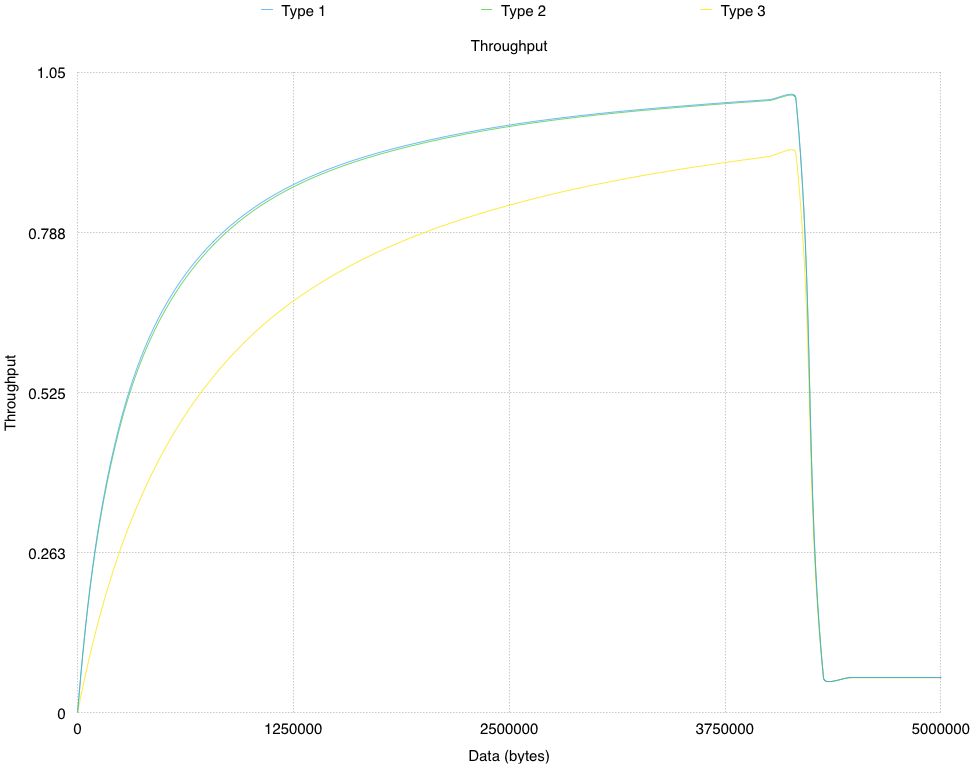
\includegraphics[width=145mm]{7/graph_model_nuim.png}
\caption{Xeon 5130: prediction of throughput of copying data in inter-thread communication}
\label{graph_model_nuim}
\end{figure}

Similarly, figure \ref{graph_model_ichec} renders throughput $n / d_{comm\_XeonE5}$. The throughput increases with the size of the buffer, until it reaches a maximum value, which is determined by the access time to main memory. The slope of the curve changes as the buffer size reaches the L1, L2, and L3 cache sizes of 32768 B, 262144 B and 32000064 B respectively.

\begin{figure}[ht!]
\centering
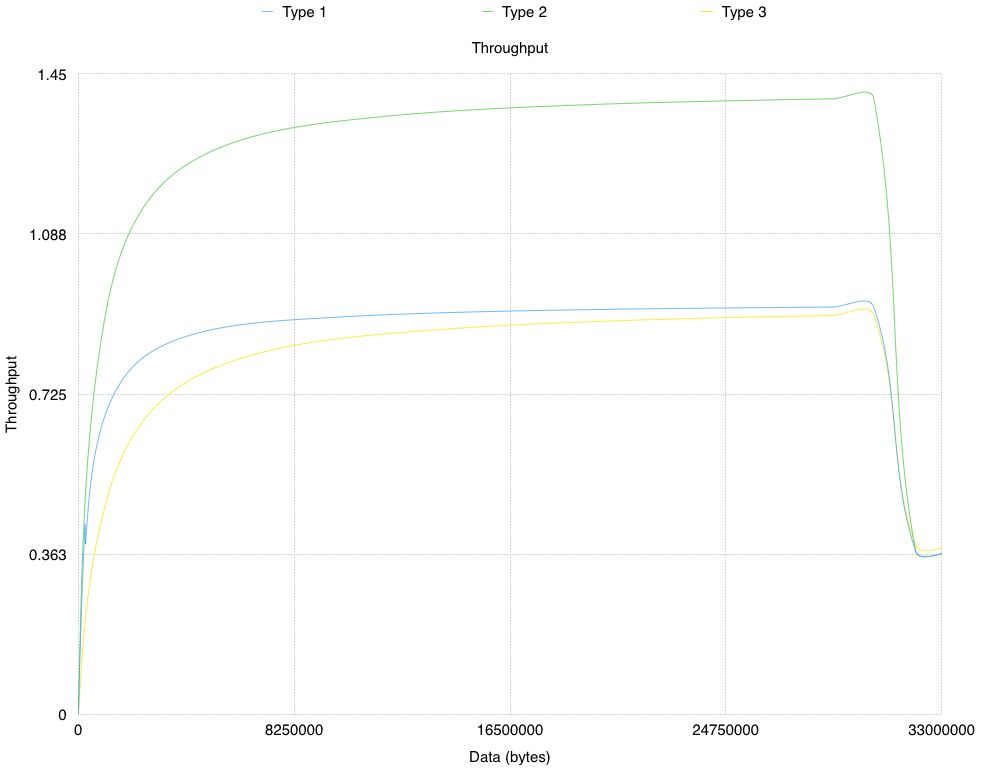
\includegraphics[width=145mm]{7/graph_model_ichec.png}
\caption{Xeon E5-2695 v2: prediction of throughput of copying data in inter-thread communication}
\label{graph_model_ichec}
\end{figure}

This model may be applied to inter-thread communication of any type in any multi-core system with similar to discussed in this project architecture with multiple levels of cache. The equations \ref{eq:discussion9} and \ref{eq:discussion10} and figures \ref{graph_model_nuim} and \ref{graph_model_ichec} presented in this section discuss the applicability of the model to two specific architectures: the Xeon 5130 and the Xeon E5-2695 v2. The next session discusses data that was measured by running the application-level experiments (described in section \ref{app_design}) and compares achieved results with the predictions made by quantifying the model.

\section{Evaluation of the Model}

Data measured through performing Experiment 2, Experiment 3, and Experiment 4 is used to verify the model's predictions of the impact of the cache on inter-thread communication. These experiments outline behaviour of the cache in a real-life setting.

As discussed in section \ref{results_app_experiments}, certain unexpected behaviour was observed when the amount of shared data exceeded 32.0435 MB while executing experiments on both the Xeon 5130 and the Xeon E5-2695 v2. The maximum value on the x-axis in the graph \ref{graph_model_nuim} is 4.75 MB and in case of the graph \ref{graph_model_ichec} it is 31.5MB. Nevertheless, as could be observed by examining the equations \ref{eq:discussion9} and \ref{eq:discussion10}, the function $d_{comm\_Xeon5130}$ has a linear nature for all values of $n$ where $n > 4194304$ (4194304 bytes is the size of the L2 caches). Similarly, the function $d_{comm\_XeonE5}$ also has a linear nature for all values of $n$ where $n > 30720000$ (30720000 bytes is the size of the L3 cache), and all lines on both graphs flatten out after $n$ reaches the size of the last level of cache.

To answer the \textit{RQ4}: cross-examining the graphs \ref{App_experiment_1_throughput_dirty_nuim} and \ref{App_experiment_1_throughput_dirty_ichec} that show throughput for both machines and the figure \ref{graph_model_nuim} and \ref{graph_model_ichec} that plot the equations of the model, shows that the developed model is capable of giving an accurate description of the impact of cache on data-sharing in inter-thread communication. Such model may be used in a cache-aware scheduler. However, there are a number of noticeable differences between the predictions of the model and the real-life results.

\subsection{Accuracy of the Model}

Figures from lmbench incorporate overhead caused by events like interrupts and and page faults. Hence values for latency measured from that benchmarking suite are always higher than (or equal to) the actual readings that can be observed in a laboratory setting where no overhead can be seen. This thesis focuses on the impact of the cache on inter-thread communication in multi-threaded applications that may be seen in the industry. One cannot totally isolate a multi-threaded programme and remove all overhead from the OS. Therefore, results from running experiments in a not fully-isolated environment are of high value. 

The main difference is in the magnitude of throughput. For example, the model shows that exchanging 1280064 bytes of data (1.22 MB) between two threads that reside on different cores of the same chip in the Xeon 5130 should take 1477750 ns, which implies that the value of throughput in this situation should be 0.87. Measuring this situation in the laboratory setting showed that such exchange takes 892488 ns, which is about 40\% times faster than the predicted value, and the reported value of throughput is 1.45.

The model proved to be overly-pessimistic. It could be caused by the inability of the laboratory setting to isolate the experiments from the overhead from the OS. Such advanced technologies as Intel's Advanced Smart Cache may also affect the results (discussed in section \ref{possibleeffects}), but modelling their behaviour is not in the scope of this research. Also, the values of latency that were measured by using lmbench cannot be fully trusted. The tool does not eliminate overhead caused by occurrence of such events as interrupts and page faults. Additionally, this study focuses on the average values of timing measurements. All experiments exhibited extremely large amounts of overhead during their execution, especially during first runs. An attempt to predict the amount of time taken by such events was undertaken, but, the high values of standard deviation reported for both interrupts/context switches and page faults (refer to section \ref{resultsDurationIntPf}) indicate that modelling behaviour of such events is overly-complicated and that it could not be performed in the given laboratory environment. A large decrease of throughput, when data that is shared between two threads exceeds the size of the last level of cache, was observed on both the Xeon 5130 and the Xeon E5-2695 v2. It is an expected result since latency of writing and reading data to/from main memory is much larger than may be observed when caches are used.

The proposed model has a linear or close to linear format for all levels of memory discussed. The plots of data that were achieved by running the experiments have more unpredictable and much more complicated nature, especially in case of the Xeon E5-2695 v2.

\subsection{Implications for Scheduling}

To address the research questions \textit{RQ1} and \textit{RQ2}, the model was able to predict that allocating threads to different cores of the same chip does not yield any noticeable benefits in the writer/reader scenario outlined in the project. The measured result showed that throughput, which can be achieved by scheduling a thread on a different core of the same die, is almost fully identical to what may be measured by pinning both the writing and the reading threads on the same core that has a private Level 1 cache. Similarly, on both graphs \ref{App_experiment_1_throughput_dirty_nuim} and \ref{App_experiment_1_throughput_dirty_ichec}, the lines that represent throughput of communication between threads that are executed by different chips are distinctly ``under" the lines that show throughput achieved during communication of Type 1 and Type 2 nature.

Performance of all three types of scheduling (Type 1: both threads are placed on the same core; Type 2: threads are put on different cores on the same chip; Type 3: threads are scheduled on different chips), as measured in the experiments, can be compared visually. Graphs \ref{thread-placement-nuim} and \ref{thread-placement-ichec} shows the impact of placement of threads for all three cases on both machines. The blue line (Type 1) serves as a base case. Other two lines (green for Type 2 and yellow for Type 3) show the impact relative to the base case, i.e. the differences in latency of scheduling two threads. If the difference is negative, one may conclude that the base case (Type 1) scheduling algorithms has an advantage, it is faster. Both plots feature the moving average trending lines to support understanding of the relations.

\begin{figure}[ht!]
\centering
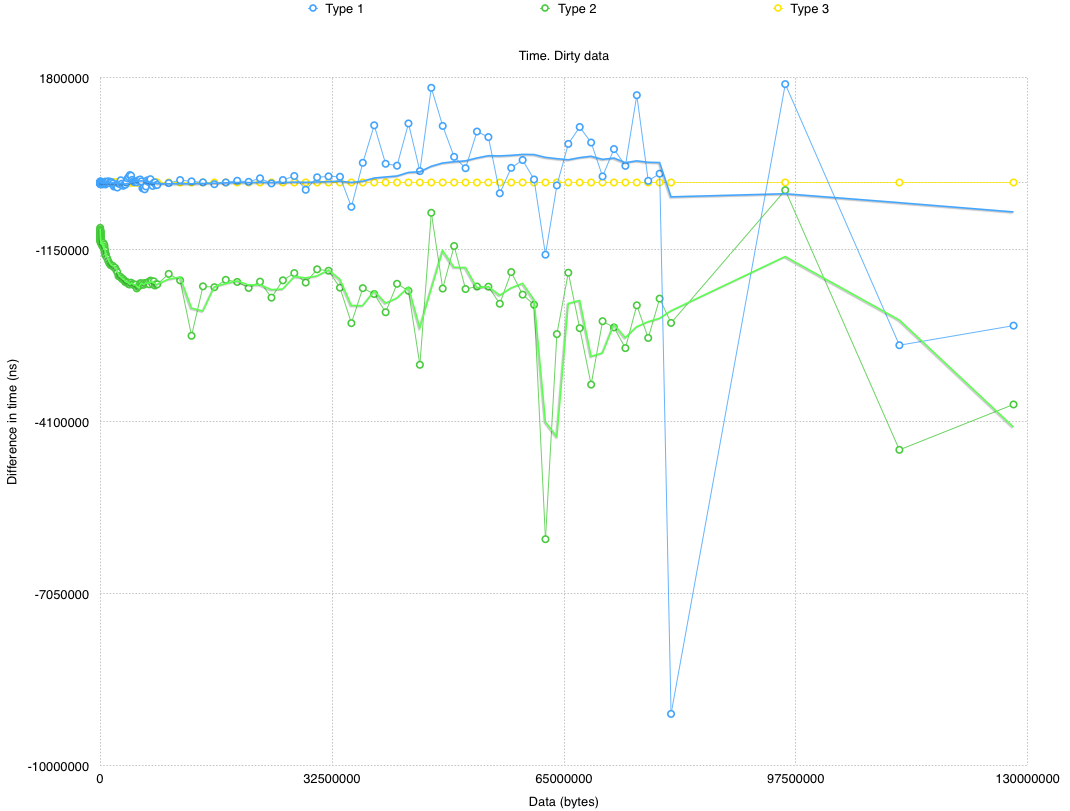
\includegraphics[width=145mm]{7/thread-placement-nuim.png}
\caption{Performance of three ways of scheduling threads, Xeon 5130}
\label{thread-placement-nuim}
\end{figure}

Figure \ref{thread-placement-nuim} shows that the impact of scheduling threads that are engaged in active exchange of data on different cores of the same chip is small (difference: 7.9 $\mu$s or 5\%); in case of placing threads on difference dies, the overhead is large (difference: 1.3 ms or 37\%). Both of these values were measured for the buffer size that is equal to the size of L2 cache in the CPU. There is no significant difference between scheduling threads on the same core and on different cores inside of one chip when less than 30 MB of data is exchanged between threads. When this threshold is reached, placing the receiving thread on a different core results in the increase of the speed of the programme by close. Scheduling the receiving thread on a different core in the same chip for more than around 70 MB of data exchanged between threads leads to the decreased speed of execution. 

Figure \ref{thread-placement-ichec} shows that the same conclusion may be derived: the impact of placing threads on different cores of the same chip in the described scenario is small (difference: 8.9 $\mu$s or 1\%) and scheduling threads on different chips if costly (difference: 1.6 ms or 15\%). Both of these values were measured for the buffer size that is equal to the size of L3 cache in the CPU. Both graphs exhibit positive and negative impact for Type 2 and Type 3 scheduling algorithms: it may be explained by the interference of the OS. A few outliers that are seen on the graphs are also caused by the interference of the Operating System. Examining the figures shows that scheduling both the sending and the receiving threads on different chips has a large impact on the speed of execution. The model gives similar predictions.

\begin{figure}[ht!]
\centering
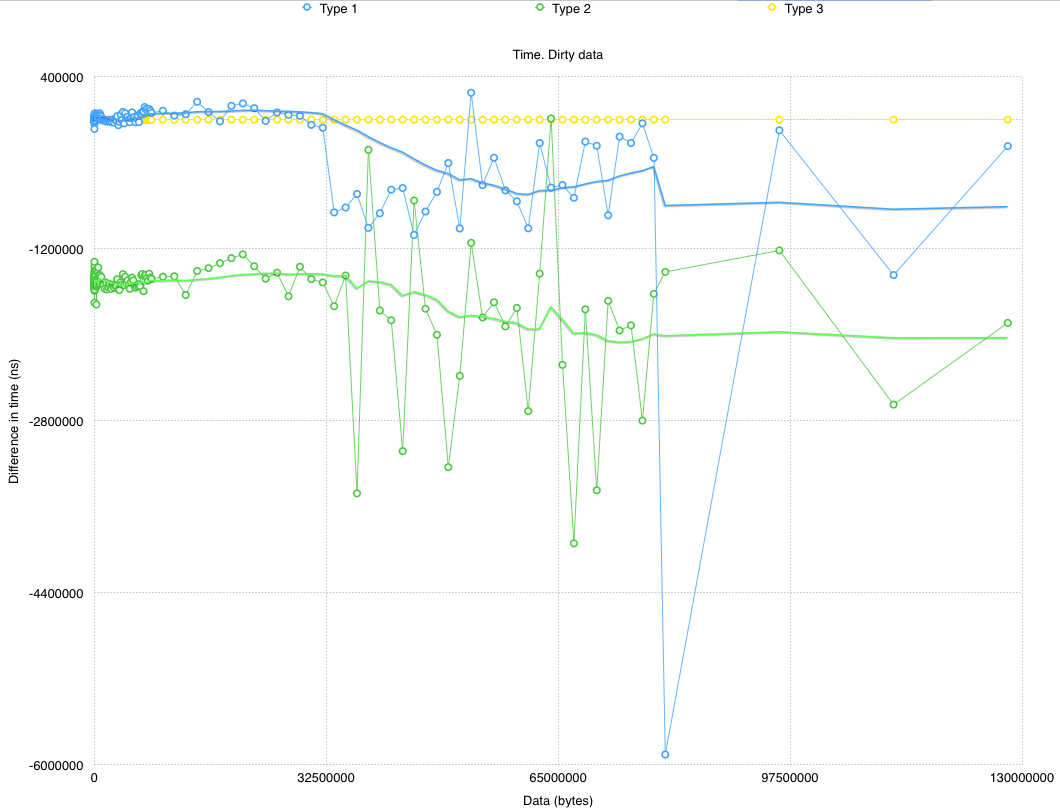
\includegraphics[width=145mm]{7/thread-placement-ichec.png}
\caption{Performance of three ways of scheduling threads, Xeon E5-2695 v2}
\label{thread-placement-ichec}
\end{figure}

It implies that executing threads that share a large amount of data on different processor chips results in decreased performance, and decreases speed of execution. Therefore, \textit{RQ} may be answered: yes, in a situation where a ``sending" and a ``receiving" threads exchange data, a scheduler should take where a receiving thread is scheduled into account.

Cache does have a large impact on the speed of programmes that have threads that are executed by different units of computation (cores or processor chips). To answer the research question \textit{RQ3}, the results received in this study may be used to provide a grounding for creation of a cache-aware scheduler that by using a theoretical model, such as the one proposed in the study, will be able to increase the speed of execution of multi-threaded programmes that have threads that are engaged in inter-thread communication. However, the proposed model needs to be fine-tuned and such aspects of cache as associativeness, differences in latency of reading and writing data and pipelining must be incorporated into the equations. There are a number of possible effects that the model does not cater for.

\section{Possible Effects not Included in the Model}
\label{possibleeffects}

The model focuses on Write-back caches (described in section \ref{cacheLit}). In a Write-through cache, data is mostly read from main memory. A reader in the sender-reader scenario discussed in the thesis would be almost guaranteed to read information, that is exchanged between threads, from main memory, and not from caches. The cache size becomes irrelevant to the speed of a programme.

One technique that is employed in many modern-day computers is data prefetching (described in section \ref{cacheLit}). It is not clear if such technology was enabled on the servers used in the study. Table \ref{prefetching1} shows what the fetch cycle would look like on the Xeon 5130 (with an assumption that the read instructions are pipelined from the i-cache\footnote{Instruction cache.}, and the biggest load comes from d-cache\footnote{Data cache.} reads) if the data cache prefetching is active. Optimum pipleining is assumed.

\begin{table*}[h]
\caption{Fetch cycle with active data prefetching on Xeon 5130}
\begin{tabular}{ll}
Time & Activity                                                                                         \\
0    & CPU read. Cache miss. Start cache line fetch from Level 2 (2 cache lines)                               \\
7.0  & First cache line fetch complete. Read complete (8 bytes) \\
 & Next read instruction starts execution \\
8.5  & Read complete (8 bytes)                                                                          \\
10.0 & Read complete (8 bytes)                                                                          \\
11.5 & Read complete (8 bytes). Cache miss on next read                                                 \\
13.0 & Second cache line complete. Read complete (8 bytes) \\
 & Next read instruction starts execution      \\
14.0 & Read complete (8 B)                                                                              \\
16.0 & Read complete (8 bytes)                                                                          \\
17.5 & Read complete (8 bytes)                                                                         
\end{tabular}
\label{prefetching1}
\end{table*}

Table \ref{prefetching2} shows a fetch cycle for a single cache line. Again, optimum pipleining is assumed.

\begin{table*}[h]
\caption{Single line fetch with no active data prefetching on Xeon 5130}
\begin{tabular}{ll}
Time & Activity                                                                                 \\
0    & CPU read. Cache miss. Start cache line fetch from Level 2 (1 cache line)                        \\
7.0  & Cache line fetch complete. Read complete (8 bytes)\\
 & Next read instruction starts execution \\
8.5  & Read complete (8 bytes)                                                                  \\
10.0 & Read complete (8 bytes)                                                                  \\
11.5 & Read complete (8 bytes). Cache miss on next read                                          \\
18.5 & Cache line fetch complete. Read complete (8 bytes)\\
 & Next read instruction starts execution \\
20.0 & Read complete (8 bytes)                                                                  \\
21.5 & Read complete (8 bytes)                                                                  \\
23.0 & read complete (8 bytes). Cache miss                                                  
\end{tabular}
\label{prefetching2}
\end{table*}

This means that reading 64 bytes (1 cache line) will take 18.5 ns as opposed to 23.0 ns. Hence model can be closer to the real-world results, it is less ``pessimistic". In this case the reported by the model latency is 10 - 20\% smaller than what is measured in the experiments.

Modern Intel processors also utilise the \textit{Advanced Smart Cache} technology \cite{Doweck2006}. This feature allows high bandwidth applications to borrow bandwidth of Level 1 to Level 2 cache from another core with a shared L2 cache. The hardware asks to allocate the full L2 or L3 cache to the application, if the other unit of computation is idle. It enables to reduce the cache miss ratio. Intel reports that it allows to achieve a constant rate of 2 clock-cycles per operation on one cache line \cite{Doweck}. In reality, is is not always a case because of other processes that take place in the system. Table \ref{prefetching3} shows what a fetch cycle would look like in this case (optimum pipelining is assumed).

\begin{table*}[h]
\caption{Fetch cycle when Advanced Smart Cache is enabled on Xeon 5130}
\begin{tabular}{ll}
Time & Activity                                                                                 \\
0    & CPU read. Cache miss. Start cache line fetch from Level 2 (fetching 2 cache \\
 & lines at once using the other core's bandwidth)                   \\
7.0  & Fetch of both cache lines completes. Read complete (8 bytes)\\
 & Next read instruction starts execution \\
8.5  & Read complete (8 bytes)                                                                  \\
10.0 & Read complete (8 bytes)                                                                  \\
11.5 & Read complete (8 bytes)                                          \\
18.5 & Read complete (8 bytes) \\
20.0 & Read complete (8 bytes)                                                                  \\
21.5 & Read complete (8 bytes)                                                                  \\
23.0 & Read complete (8 bytes)                                                  
\end{tabular}
\label{prefetching3}
\end{table*}

Then, instruction pipelining (instruction parallelism), where multiple instructions can be executed at the same time, may influence the behaviour of the model. Because optimum pipelining is assumed in the model, instruction pipelining is unlikely to be a factor in the performance of the model. Parallel instruction execution does not allow faster throughput that is supported by the cache; it is not a significant factor for the accuracy of the model. The cache bus may also be an additional factor.

\section{Survey of Similar Results}

A number of similar to was is described in the thesis experiments are reported in an article \cite{Molka2009a}. It investigates the latency of cache on a Nehelam architecture\footnote{A 45--nm architecture that was used by Intel during 2008 -- 2011.}. The finding reported in the article cannot be used to compare what is descried in this thesis since the Woodcrest\footnote{A 65--nm architecture that was used by Intel during 2006 -- 2008.} and Ivy Bridge\footnote{A 22--nm architecture that is currently used by Intel.} architectures are utilised in the experimental environment. Authors of \cite{KentMilfeldKazushigeGotoAviPurkayastha2007} also discuss results of a number of benchmarks that evaluate speed of multi-threaded programmes. They focus on the changes in the architecture of CPUs that are caused by increasing clock speed and usage of multiple cores. Both shared and independent cache systems are evaluated. It was reported that the locality of data in independent cache systems has to be ensured by operations that can cost as many as 5000 clock cycles each. It is a very large overhead for such operation.

Data that is reported from the experiments has a dependency on the figures of cache latency measured with lmbench. As described in section \ref{results_lmbench}, such numbers could not be fully trusted, due to the closed nature and the age of the benchmark. A report of similar measurements performed with this tool may be found in \cite{Prakash2007}. The paper reports memory-load latency for the Intel Core 2 Duo E6400 processor. Despite the difference in the architectures, the curves of graphs reported in the publication can be related to the findings in this project. The findings are similar to what is reported in this thesis.

Modelling behaviour of cache is a difficult undertaking \cite{Shen2000,Putigny2014}. The paper \cite{Putigny2014} discusses that automatic hardware mechanisms (such as prefetchers and cache coherence protocols) improve performance, but they also make modelling of the impact of the cache more difficult. Many sources provide rules for compiler optimization through analysing data locality by means of computing stack distances\footnote{\textit{Stack distance} -- a depth of a stack, that a reference needs to be extracted from.} \cite{Vera2004,Cacaval2003}, such analysis is easier to conduct, since behaviour of the aforementioned optimisation techniques can be ignored, but it yields limited conclusions.

% ---------------------------------------------------------------------------
% ----------------------- end of thesis sub-document ------------------------
% ---------------------------------------------------------------------------               % discussion of results


% this file is called up by thesis.tex
% content in this file will be fed into the main document

\chapter{Conclusions and Future Work} % top level followed by section, subsection

% ----------------------- paths to graphics ------------------------

% change according to folder and file names
\ifpdf
    \graphicspath{{8/figures/PNG/}{8/figures/PDF/}{8/figures/}}
\else
    \graphicspath{{8/figures/EPS/}{8/figures/}}
\fi

% ----------------------- contents from here ------------------------

This project evaluated the impact of cache on inter-thread communication in multi-threaded environments. Then, it assessed whether a scheduler needs to take such impact into account, when receiving threads are scheduled. This study involved creation of a model that describes inter-thread communication. Additionally, a taxonomy of such communication in multi-core systems was developed. Five experiments were designed to provide information necessary to quantify and verify the model. Two workstations that are powered by multi-chip processors Intel Xeon 5130 and Intel Xeon E5-2695 v2 were chosen for executing the experiments. The processors have different memory hierarchies, which allowed to receive results that permitted to test the validity of the model in different environments.

A scenario described in the thesis, where a ``sending" thread (producer) writes data and a ``receiving" thread (consumer) reads data is possible in a real-life setting. The findings show that in such situation \textit{scheduling the receiving thread on a separate chip decreases the speed of execution of a multi-threaded programme} (by up to 37\% on Xeon 5130 and by up to 15\% on Xeon E5-2695 v2). \textit{Scheduling both threads on different cores of the same chip does not give any noticeable advantages}, i.e. the execution time is close to the base-case scenario where both threads are run on a single core (5\% difference on Xeon 5130 and 1\% difference on Xeon E5-2695 v2). Therefore, the fundamental conclusion may be defined as: \textit{in ``sender" - ``receiver" programmes, a scheduler needs to take where a receiving thread is scheduled into account}.

For both the Xeon 5130 and the Xeon E5-2695 v2, the model was able to describe throughput of inter-thread communication. The model is capable of outlining patterns of latency and throughput for all three types of communication as described in the taxonomy: 1) where two threads that have been scheduled to the same core exchange data; 2) when two threads that reside on two cores on the same die communicate with each other; 3) where two threads that have been put on two different chips exchange data.

The proposed model predicts close to linear nature for all levels of memory that it describes. Conducting experiments showed that in reality inter-thread communication is much more complicated and requires further modelling and analysis. Modelling cache behaviour is difficult \cite{Putigny2014}. Due to unavailability of detailed documentation of the underlying systems in modern-day processors, the performance model needs to abstract multiple aspects of the work of modern-day CPUs. Very little work on modelling of cache behaviour is done in the scientific community. Most only discuss simulations and provide no background analysis \cite{Heidelberger1990,Archibald1986,Zhao2011}. This thesis shows how difficult it is to model such behaviour.

Data measured in the experiments can be considered dependable due to its nature, the experiments were run directly on the hardware. Because of the time limitation, formal methods could not be used to verify dependability of the experimental environment and achieved results.

\section{Limitations}

The accuracy of measured data can be improved, if the experiments were run as real-time process, which would have involved recompiling the Linux kernel in the given setting. The laboratory set-up used for conducting the experiments did not permit to do that easily. Also, it is believed that utilisation of the parallelised version of the \textit{RDTSC} instruction -- \textit{RDTSCP} -- or deterministic performance counters \cite{Weaver2013} will improve accuracy of measuring time. It will increase the level of dependability of achieved results, and it may permit usage of results that were measured in Experiment 1 (the overhead from the OS could not be eliminated, and the results were too ``noisy" to be used). The accuracy and precision of results could be improved if direct access to the servers was granted.

This work discusses write-back caches. The reported results and predictions of the model will not hold for write-through caches (another commonly-used cache architecture), since the underlying behaviour of such caches is fundamentally different. When a write-through cache is used, data is written to caches and main memory, as opposed to just caches; it is not discussed in the model.

Further, the proposed model ignores the aspect of cache associativity. It describes behaviour of only direct mapped caches. Adding support for fully associative and n-way set associative caches will improve the applicability of the model and the accuracy of scheduling decisions made based on its predictions.

\section{Future Work}

The key aim of any future work should focus on performing a similar study in a more complicated environment. This project focused on the case where a receiving threads runs immediately after a sending thread. The model may be used as a base for development of a more complete mathematical description of the processes that take place when multiple threads exchange information in a multi-core environment. Future work needs to extend reported results by performing experiments with thousands or millions of receiving and sending threads. A scenario that may commonly be seen in the Openet's area of expertise: solutions for analytics of telecommunications systems. The model also needs to be refined to provide more precise predictions that yield more accurate scheduling decisions. The refinement may include support for a larger number of memory hierarchies, prefetching, instruction parallelism, as well as other advanced techniques employed in modern-day processors. Such refinement will allow to create a more general model that will be applicable to a larger range of hardware.

Further work may also involve testing the model with other scenarios of inter-thread communication and finishing the cross-platform support of the experimental environment (receiving data on different systems will be beneficial for development of a scheduler that can be run on different platforms). Additionally, the described experiments can be run in set ups that have distinctly different, to what is used in the study, hardware. One may decide to choose processors from other than Intel manufactures (e.g. AMD), since they often organise computer memory differently.

Then, to improve dependability of the system and data that is measured in the experiments, a number of tools that are used in the industry and research may be used \cite{Woodcock2009}. In particular, VeriFast\footnote{\url{http://people.cs.kuleuven.be/~bart.jacobs/verifast/}} may be utilised in the project, as it is currently one of the front-runners in the industry \cite{Philippaerts2013} that has support for semi-automatic verification of software written in C. It will allow to prove that the code behind the experimental environment and the experiments is reliable and bug-free, which in turn will increase the dependability of received results.

The author plans to continue work on this project, fine-tune the proposed model by performing the described experiments in other settings and develop a cache-aware scheduler that could be deployed to Linux-based systems. Such further work will allow to measure the applicability of such scheduler and see whether the results correlate to what is reported in the thesis.

% ---------------------------------------------------------------------------
%: ----------------------- end of thesis sub-document ------------------------
% ---------------------------------------------------------------------------        % conclusion



% --------------------------------------------------------------
%:                  BACK MATTER: appendices, refs,..
% --------------------------------------------------------------

% the back matter: appendix and references close the thesis


%: ----------------------- bibliography ------------------------

% The section below defines how references are listed and formatted
% The default below is 2 columns, small font, complete author names.
% Entries are also linked back to the page number in the text and to external URL if provided in the BibTex file.

% PhDbiblio-url2 = names small caps, title bold & hyperlinked, link to page 
\begin{multicols}{2} % \begin{multicols}{ # columns}[ header text][ space]
\begin{tiny} % tiny(5) < scriptsize(7) < footnotesize(8) < small (9)

\bibliographystyle{Latex/Classes/PhDbiblio-url2} % Title is link if provided
\renewcommand{\bibname}{References} % changes the header; default: Bibliography

\bibliography{9_backmatter/references} % adjust this to fit your BibTex file

\end{tiny}
\end{multicols}

% --------------------------------------------------------------
% Various bibliography styles exit. Replace above style as desired.

% in-text refs: (1) (1; 2)
% ref list: alphabetical; author(s) in small caps; initials last name; page(s)
%\bibliographystyle{Latex/Classes/PhDbiblio-case} % title forced lower case
%\bibliographystyle{Latex/Classes/PhDbiblio-bold} % title as in bibtex but bold
%\bibliographystyle{Latex/Classes/PhDbiblio-url} % bold + www link if provided

%\bibliographystyle{Latex/Classes/jmb} % calls style file jmb.bst
% in-text refs: author (year) without brackets
% ref list: alphabetical; author(s) in normal font; last name, initials; page(s)

%\bibliographystyle{plainnat} % calls style file plainnat.bst
% in-text refs: author (year) without brackets
% (this works with package natbib)


% --------------------------------------------------------------

%: Declaration of originality
\cleardoublepage\makeatletter\@openrightfalse\makeatother
\begin{appendices}

\chapter{Source code of \textit{pagefaults\_fopen.c}}
\label{app:listingTestPagefault}

\begin{lstlisting}[
language=C
]
#include <stdio.h>
#include <stdlib.h>
#include <unistd.h>
#include <string.h>

unsigned long long get_page_fault(int choice);
char * file_to_string(char *f);

struct proc_stats {
	int pid;			// %d
	char comm[256];		// %s
	char state;			// %c
	int ppid;			// %d
	int pgrp;			// %d
	int session;		// %d
	int tty_nr;			// %d
	int tpgid;			// %d
	unsigned long flags;	// %lu
	unsigned long long minflt;	// %lu
	unsigned long long cminflt;	// %lu
	unsigned long long majflt;	// %lu
	unsigned long long cmajflt;	// %lu
	unsigned long utime;	// %lu
	unsigned long stime; 	// %lu
	long cutime;		// %ld
	long cstime;		// %ld
	long priority;		// %ld
	long nice;			// %ld
	long num_threads;		// %ld
	long itrealvalue;		// %ld
	unsigned long starttime;	// %lu
	unsigned long vsize;	// %lu
	long rss;			// %ld
	unsigned long rlim;		// %lu
	unsigned long startcode;	// %lu
	unsigned long endcode;	// %lu
	unsigned long startstack;	// %lu
	unsigned long kstkesp;	// %lu
	unsigned long kstkeip;	// %lu
	unsigned long signal;	// %lu
	unsigned long blocked;	// %lu
	unsigned long sigignore;	// %lu
	unsigned long sigcatch;	// %lu
	unsigned long wchan;	// %lu
	unsigned long nswap;	// %lu
	unsigned long cnswap;	// %lu
	int exit_signal;		// %d
	int processor;		// %d
	unsigned long rt_priority;	// %lu
	unsigned long policy;	// %lu
	unsigned long long delayacct_blkio_ticks;	// %llu
};

int main(int argc, const char ** argv) {
	unsigned long long pageFaultsB = get_page_fault(1);

	// Read file
	FILE *fp;

	// Open file.
	if ((fp = fopen("/proc/interrupts", "r")) == NULL) {
		return (-1);
	}

	//Close the file if still open.
	if (fp) {
		fclose(fp);
	}
	// Finished reading file

	unsigned long long pageFaultsA = get_page_fault(1);

	printf("1st time /proc/interrupts: Before: %llu After:
	    %llu\n", pageFaultsB, pageFaultsA);

	pageFaultsB = get_page_fault(1);

	// Open file.
	if ((fp = fopen("/proc/interrupts", "r")) == NULL) {
		return (-1);
	}

	//Close the file if still open.
	if (fp) {
		fclose(fp);
	}
	// Finished reading file

	pageFaultsA = get_page_fault(1);

	printf("2nd time /proc/interrupts: Before: %llu After:
	    %llu\n", pageFaultsB, pageFaultsA);

	pageFaultsB = get_page_fault(1);

	// Open file.
	if ((fp = fopen("/proc/iomem", "r")) == NULL) {
		return (-1);
	}

	//Close the file if still open.
	if (fp) {
		fclose(fp);
	}
	// Finished reading file

	pageFaultsA = get_page_fault(1);

	printf("1st time /proc/iomem: Before: %llu After:
	    %llu\n", pageFaultsB, pageFaultsA);

	pageFaultsB = get_page_fault(1);

	// Open file.
	if ((fp = fopen("/proc/iomem", "r")) == NULL) {
		return (-1);
	}

	//Close the file if still open.
	if (fp) {
		fclose(fp);
	}
	// Finished reading file

	pageFaultsA = get_page_fault(1);

	printf("2nd time /proc/iomem: Before: %llu After:
	    %llu\n", pageFaultsB, pageFaultsA);

	char * str1 = file_to_string("/proc/interrupts");
	char * str2;


	while (strcmp(str1, str2) != 0) {
		pageFaultsB = get_page_fault(1);
		str2 = file_to_string("/proc/interrupts");
		pageFaultsA = get_page_fault(1);
	}

	printf("/proc/interrupts changed: Before: %llu After:
	    %llu\n", pageFaultsB, pageFaultsA);
}

int read_stat(char * filename, int pid, struct proc_stats *s) {
#ifndef __APPLE__
	const char *format =
		"%d %s %c %d %d %d %d %d %lu %lu %lu %lu %lu %lu %lu
		   %ld %ld %ld %ld %ld %ld %lu %lu %ld %lu %lu %lu
		   %lu %lu %lu %lu %lu %lu %lu %lu %lu %lu %d %d %lu
		   %lu %llu";
	FILE *fp;

	fp = fopen(filename, "r");
	if (fp) {
		if (42
		== fscanf(fp, format, &s->pid, s->comm, &s->state,
	    &s->ppid, &s->pgrp, &s->session, &s->tty_nr,
	    &s->tpgid, &s->flags, &s->minflt, &s->cminflt,
	    &s->majflt, &s->cmajflt, &s->utime, &s->stime,
		&s->cutime, &s->cstime, &s->priority, &s->nice,
		&s->num_threads, &s->itrealvalue,
		&s->starttime, &s->vsize, &s->rss, &s->rlim,
		&s->startcode, &s->endcode, &s->startstack,
		&s->kstkesp, &s->kstkeip, &s->signal, &s->blocked,
		&s->sigignore, &s->sigcatch, &s->wchan, &s->nswap,
		&s->cnswap, &s->exit_signal, &s->processor,
		&s->rt_priority, &s->policy, 
		&s->delayacct_blkio_ticks)) {
			if (fp) {
				fclose(fp);
			}
			return 1;
		} else {
			if (fp) {
				fclose(fp);
			}
			return 0;
		}
	} else {
		return 0;
	}
#else
	return -1;
#endif
}

// 1 - minor, 2 - major
unsigned long long get_page_fault(int choice) {
#ifndef __APPLE__
	struct proc_stats statsData;
	int self = getpid(); // Process ID

	char buf[256];
	sprintf(buf, "/proc/%d/stat", self);

	// Read data from the stats file
	read_stat(buf, self, &statsData);

	if (choice == 1) {
		return statsData.minflt;
//		return statsData->cminflt);

	} else if (choice == 2) {
		return statsData.majflt;
//	    return statsData->cmajflt;
	}

#else
	return -1;
#endif
}

// For storing contents of the file.
static char result[8][8 * 1024]; 
// Counter of how many files have been stored in result.
static int cycle = 0; 

char * file_to_string(char *f) {
	FILE *fp;
	char temp[512];

	cycle++;
	if (cycle == 8)
		cycle = 0;

	// Open file.
	if ((fp = fopen(f, "r")) == NULL) {
		return (char *) (-1);
	}

	// Initialise the result
	result[cycle][0] = 0;

	// Search for str and extract numeric.
	while (fgets(temp, 512, fp) != NULL) {
		strcat(result[cycle], temp);
	}

	// Check if there is a memory leak. 
	if (strlen(result[cycle]) > 8 * 1024) {
		printf("Memory error - strlen(result)==%lu,
		    file size==%d\n", strlen(result[cycle]),
		    8 * 1024);
		if (fp) {
			fclose(fp);
		}
		exit(1);
	}

	//Close the file if still open.
	if (fp) {
		fclose(fp);
	}

	return &result[cycle][0];
}
\end{lstlisting}

\chapter{Source code of \textit{clock-gettime\_test.c}}
\label{app:listingTestClockGetTime}

\begin{lstlisting}[
language=C
]
#include <stdio.h>
#include <stdlib.h>
#include <unistd.h>
#include <signal.h>
#include <inttypes.h>
#include <cpuid.h>
#include <sys/prctl.h>
#include <linux/prctl.h>
#include <time.h>

// Get the process' ability to use the
// timestamp counter instruction
#ifndef PR_GET_TSC
#define PR_GET_TSC 25
#define PR_SET_TSC 26
// Allow the use of the timestamp counter
# define PR_TSC_ENABLE 1 
// Throw a SIGSEGV instead of reading the TSC
# define PR_TSC_SIGSEGV	2 
#endif

#define LOOPS 1024

const char *tsc_names[] = { [0] = "[not set]",
    [PR_TSC_ENABLE] = "PR_TSC_ENABLE",
    [PR_TSC_SIGSEGV] = "PR_TSC_SIGSEGV", };

void sigsegv_cb(int sig) {
	int tsc_val = 0;

	printf("[ SIG_SEGV ]\n");
	printf("prctl(PR_GET_TSC, &tsc_val); ");
	fflush(stdout);

	if (prctl(PR_GET_TSC, &tsc_val) == -1)
		perror("prctl");

	printf("tsc_val == %s\n", tsc_names[tsc_val]);
	printf("prctl(PR_SET_TSC, PR_TSC_ENABLE)\n");
	fflush(stdout);
	if (prctl(PR_SET_TSC, PR_TSC_ENABLE) == -1)
		perror("prctl");

	printf("clock_gettime() == ");
}

int main(int argc, char **argv) {
	int tsc_val = 0;
	struct timespec r1, r2, r3, r4, temp;
	struct timespec rs[LOOPS];
	int i, j;
    
    // Make sure there is no I/O pending from
    // this process
	sleep(1); 
	get_time(&r1);
	get_time(&r2);
	get_time(&r3);
	get_time(&r4);
	// This (might) ensure that we have a full
	// time quantum to execute in - as we get
    // re-scheduled after the sleep
	usleep(10); 
	// the next few instructions get pre-loaded
	// into i-cache
	get_time(&r1);
	get_time(&r2);
	get_time(&r3);
	get_time(&r4);

	printf("%llu %llu %llu %llu\n", (unsigned long long)
	    r1.tv_nsec, (unsigned long long) r2.tv_nsec, 
	    (unsigned long long) r3.tv_nsec,
	    (unsigned long long) r4.tv_nsec);
	printf("%llu %llu %llu\n", (unsigned long long)
	    (r2.tv_nsec - r1.tv_nsec), (unsigned long long)
	    (r3.tv_nsec - r2.tv_nsec), (unsigned long long)
	    (r4.tv_nsec - r3.tv_nsec));

	printf("clock_gettime() == ");
	fflush(stdout);

    // Make sure there is no I/O pending from this process
	sleep(1); 
	// Use 2 loops to preload the i-cache and makes sure 
	// there will be no page faults on the rs array
	for (j = 0; j < 2; j++) {
		for (i = 0; i < LOOPS; i++) {
			get_time(&rs[i]);
		}
	}
	for (i = 1; i < LOOPS; i++)
		printf("%llu ", (unsigned long long)
		    rs[i].tv_nsec - rs[i - 1].tv_nsec);

	printf("\n");
	fflush(stdout);
	exit(EXIT_SUCCESS);
}

//  Get time in nano-seconds
int get_time(struct timespec *timeStruct) {
	if (clock_gettime(CLOCK_MONOTONIC, timeStruct) == -1) {
		perror("clock getres");
		return 0;
	}
	return 1;
}
\end{lstlisting}

\chapter{Source code of the function \textit{void test\_rdtsc(void)}}
\label{app:listingTestRDTSC}

\begin{lstlisting}[
language=C
]
// Test rdtsc
void test_rdtsc(void) {
	// With CPUID
	printf("TEST OF RDTSC with CPUID\n");

	unsigned long long t[32], prev;
	int i;
	for (i = 0; i < 32; i++)
		t[i] = rdtsc_old(1);

	prev = t[0];
	for (i = 1; i < 32; i++) {
		printf("%llu [%llu]\n", t[i], t[i] - prev);
		prev = t[i];
	}

	printf("Total=%llu\n", t[32 - 1] - t[0]);

	// Without CPUID
	printf("\nTEST OF RDTSC without CPUID\n");

	for (i = 0; i < 32; i++)
		t[i] = rdtsc_old(0);

	prev = t[0];
	for (i = 1; i < 32; i++) {
		printf("%llu [%llu]\n", t[i], t[i] - prev);
		prev = t[i];
	}

	printf("Total=%llu\n", t[32 - 1] - t[0]);
}
\end{lstlisting}

\chapter{Bash code for running lmbench on the Xeon E5-2695 v2}
\label{app:listingLmbenchICHEC}

\begin{lstlisting}[
language=bash
]
#!/bin/bash
#PBS -l nodes=1:ppn=24
#PBS -l walltime=5:00:00
#PBS -N lmbench
#PBS -A nuim01
#PBS -r n
#PBS -j oe
#PBS -m bea
#PBS -M pavlo.bazilinskyy@gmail.com

cd $PBS_O_WORKDIR
OS=x86_64-linux-gnu
CONFIG=CONFIG.r1i1n5
RESULTS=results/$OS
BASE=../$RESULTS/`uname -n`
EXT=0

if [ ! -f "../bin/$OS/$CONFIG" ]
then    echo "No config file?"
        exit 1
fi
. ../bin/$OS/$CONFIG

if [ ! -d ../$RESULTS ]
then    mkdir -p ../$RESULTS
fi
RESULTS=$BASE.$EXT
while [ -f $RESULTS ]
do      EXT=`expr $EXT + 1`
        RESULTS=$BASE.$EXT
done

cd ../bin/$OS
PATH=.:${PATH}; export PATH
export SYNC_MAX
export OUTPUT
lmbench $CONFIG 2>../${RESULTS}

if [ X$MAIL = Xyes ]
then    echo Mailing results
        (echo ---- $RESULTS ---
        cat ../$RESULTS) | mail pavlo.bazilinskyy@gmail.com
fi
exit 0
\end{lstlisting}


\chapter{Source code of the main function of \textit{void test\_time\_int\_pf.c}}
\label{app:listingTestInterrupt}

\begin{lstlisting}[
language=C
]
int main(int argc, const char ** argv) {
	int k;
	long sum;
	struct timespec start, stop;
	int run = 10;

	// Record times of experiments in the run.
	unsigned long long *time = malloc(sizeof(
	    unsigned long long) * run);
	if (time == NULL) {
		printf("Error with allocating space for the array\n");
		exit(1);
	}

	// Caculate the average duration of an interrupt
	printf("INTERRUPTS\n\ntime,num\n");
	int i = 0;
	for (i = 0; i < run; ++i) {
		unsigned long long interruptsBefore;
		unsigned long long interruptsAfter;

		// Warmup
		interruptsAfter = search_in_file(
		    "/proc/interrupts", "LOC:", 1);
		interruptsBefore = interruptsAfter;

		while (interruptsBefore == interruptsAfter)
			interruptsBefore = search_in_file("
			    /proc/interrupts", "LOC:", 1);

		// Create interrupts
		do {
		    // Record time before causing the interrupt
			get_time_ns(&start);
			interruptsAfter = search_in_file(
			    "/proc/interrupts", "LOC:", 1);
		} while (interruptsAfter - interruptsBefore != 1);
        
        // Record time after causing the interrupt
		get_time_ns(&stop);
    
        // How many interrupts occurred
		int numInterrupts = interruptsAfter -
		    interruptsBefore;
		    
		// Record time with interrupts
		unsigned long long timeWithInterupts =
		    calculate_time_ns(start, stop);

		printf("%d,%llu\n", timeWithInterupts, numInterrupts);
		// Record time difference over a number of interrupts
		time[i] = timeWithInterupts / numInterrupts;
	}
	printf("1 interrupt takes (average from %d runs):
	    %llu\n", run, average_time(time, run));

	// Caculate the average duration of a page fault
	printf("\nPAGE FAULTS\n\ntime,num\n");
	for (i = 0; i < run; ++i) {
		unsigned long long pfBefore;
		unsigned long long pfAfter;

		// Warmup
		struct proc_stats stat_file =
		    get_page_fault_file();
		pfAfter = get_page_fault(stat_file, 1);
		pfBefore = pfAfter;

		while (pfBefore == pfAfter) {
			stat_file = get_page_fault_file();
			pfBefore = get_page_fault(stat_file, 1);
		}
        
        // Record time before causing a page fault
		get_time_ns(&start);

		// Create page faults
		do {
			stat_file = get_page_fault_file();
			pfAfter= get_page_fault(stat_file, 1);
		}while (pfAfter - pfBefore == 0);
    
        // Record time after causing a page fault
		get_time_ns(&stop); 

        // How many minor page faults occurred
		int numPf = pfAfter - pfBefore;
		// Record time with page faults
		unsigned long long timeWithPf =
		    calculate_time_ns(start, stop);
    
        // Record time difference over a number of page faults
		printf("%d,%llu\n", timeWithPf, numPf);
		time[i] = timeWithPf / numPf;
	}
	printf("1 interrupt takes (average from %d runs):
	    %llu\n", run, average_time(time, run));

	free(time);
	return sum;
}
}

\end{lstlisting}


\chapter{Source code of the experiment with threads residing on the same core}
\label{app:listingExperiment2}

\begin{lstlisting}[
language=C
]
/*
 * EXPERIMENT 2
 *
 */
void experiment_2(int n) {
	// Aligned array for manipulating data
	long *testAr = align_long_array(sizeof(long) * n);

	// Wrap information that has to be passed to a pthread
	struct argStructType * argStruct = malloc(sizeof(
	    struct argStructType));
	argStruct->experimentId = 2;
	argStruct->n = n;
	argStruct->testAr = testAr;

	pthread_mutex_init(&mut, NULL); // Initialise the mutex.

	// Create pthreads
	rc = pthread_create(&thread1, NULL, e2_pthread_main1,
	    (void *) argStruct);
	if (rc) {
		printf("ERROR; return code from pthread_create()
		    is %d\n", rc);
		exit(-1);
	}

	// Join threads
	pthread_join(thread1, NULL);
	pthread_join(thread2, NULL);

	// Finish
	free(testAr);
	// Free memory allocated for generic argument struct
	free(argStruct); 
	pthread_mutex_destroy(&mut);
}

// Sender. This thread sends data
void *e2_pthread_main1(void * argStruct) {
    // Pin to the first core of the first CPU.
	pin_thread_to_core(0); 
    
    // Unpack arguments
	struct argStructType *args =
	    (struct argStructType *) argStruct; 	

    // Lock mutex.
	pthread_mutex_lock(&mut); 

    // Create the 2nd thread
	rc = pthread_create(&thread2, NULL, e2_pthread_main2,
	    (void *) argStruct);
	if (rc) {
		printf("ERROR; return code from pthread_create()
		    is %d\n", rc);
		exit(-1);
	}

	// Work with  shared data
	int i = 0;
	for (i = 0; i < args->n; ++i) {
		args->testAr[i] = 3l;
	}

	pthread_mutex_unlock(&mut); // Lock mutex.

	return ((void *) 1);
}

// Receiver. This thread receives data
void *e2_pthread_main2(void * argStruct) {
    // Pin to the first core of the first CPU.
	pin_thread_to_core(0); 
    
    // Unpack arguments
	struct argStructType *args =
	    (struct argStructType *) argStruct;

    // Lock mutex.
	pthread_mutex_lock(&mut); 

	// Work with  shared data
	int i = 0;
	long temp; // For assignment of values.
	for (i = 0; i < args->n; ++i) {
		temp = args->testAr[i];
	}
    
    // Lock mutex.
	pthread_mutex_unlock(&mut); 

	return ((void *) 1);
}

\end{lstlisting}

\chapter{Makefile used to run experiments}
\label{app:listingMakefile}

\begin{lstlisting}[
language=bash
]
CC =gcc
IFLAGS =-I
WFLAG1 = -Wall
WFLAG2 = -Werror
WFLAG3 = -Wextra
WFLAGS = $(WFLAG1)
OFLAGS = -g -O0
DFLAGS = # -Doptions
UFLAGS = # Set on make command line only
CFLAGS = $(SFLAGS) $(DFLAGS) $(IFLAGS) $(OFLAGS) $(WFLAGS) $(UFLAGS)
LIBS =
DEPS =test.h hr_timer.h file_worker.h conf.h experiments.h test_env.h
OBJ  =test.o hr_timer.o file_worker.o experiments.o test_env.o

UNAME_S := $(shell uname -s)
ifeq ($(UNAME_S),Linux)
	LIBS += -lrt -lpthread -lm
endif
ifeq ($(UNAME_S),Darwin)
	DEPS += clock_gettime_mac.h
	OBJ  += clock_gettime_mac.o
endif

%.o: %.c $(DEPS)
	$(CC) -c -g -o $@ $< $(CFLAGS) $(LIBS)

test: $(OBJ)
	$(CC) -o $@ $^ $(LIBS)

.PHONY: clean

clean:
	rm -f *.o *~
\end{lstlisting}

\chapter{Average duration of interrupts and minor page faults, Xeon 5130}
\label{app:durationIntNuim}

\begin{lstlisting}[
language=bash
]
INTERRUPTS
time,num
84547,1
154798,1
84397,1
84743,1
84797,1
96676,1
101176,1
650527,1
95336,1
99946,1
1 interrupt takes (average from 10 runs): 153694

PAGE FAULTS
time,num
42207,1
41603,1
41320,1
47684,1
41624,1
41336,1
41315,1
46944,1
41336,1
41293,1
1 page fault takes (average from 10 runs): 42666
\end{lstlisting}

\chapter{Average duration of interrupts and minor page faults, Xeon E5-2695 v2}
\label{app:durationIntIchec}

\begin{lstlisting}[
language=bash
]
INTERRUPTS
time,num
315246,1
332646,1
313228,1
314809,1
319510,1
314532,1
315445,1
318588,1
368649,1
315614,1
1 interrupt takes (average from 10 runs): 322826
PAGE FAULTS
time,num
19733,1
26440,1
19987,1
23632,1
18098,1
23189,1
18420,1
18427,1
25780,1
23624,1
1 page fault takes (average from 10 runs): 21733
\end{lstlisting}

\chapter{Results of Experiment 1, filtered data, Xeon 5130}
\label{app:cycle-level-results-clean-nuim}

Information on the numbers of interrupts and minor page faults for first three runs of each iteration of the experiment is given. Selected rows were removed. The original file that contains information on all 10 runs of each of 235 sub-experiments of each iteration of the experiment and presents data on the numbers of recorded major page faults, may be found at: \url{https://github.com/Hollgam/cache-mt/tree/master/results/nuim\_clean-1-0.csv}.

\csvautolongtable{9_backmatter/xeon_clean-1-0.csv}

\chapter{Results of Experiment 1, filtered data, Xeon E5-2695 v2}
\label{app:cycle-level-results-clean-ichec}

Information on the numbers of interrupts and minor page faults for first three runs of each iteration of the experiment is given. Selected rows were removed. The original file that contains information on all 10 runs of each of 235 sub-experiments of each iteration of the experiment and presents data on the numbers of recorded major page faults, may be found at: \url{https://github.com/Hollgam/cache-mt/tree/master/results/ichec\_clean-1-0.csv}.

\csvautolongtable{9_backmatter/ichech_xeon_clean-1-0.csv}

\chapter{Results of running the memory benchmark from lmbench}
\label{app:lmbench-results}

\csvautolongtable{9_backmatter/lmbench.csv}

\chapter{Results of Experiment 2, unfiltered data, Xeon 5130}
\label{app:app-level-results-2-nuim}

Information on the numbers of interrupts and minor page faults for first three runs of each iteration of the experiment is given. Selected rows were removed. The original file that contains information on all 10 runs of each of 235 sub-experiments of each iteration of the experiment and presents data on the numbers of recorded major page faults, may be found at: \url{https://github.com/Hollgam/cache-mt/tree/master/results/nuim\_dirty-2-0.csv}.

\csvautolongtable{9_backmatter/xeon_dirty-2-0.csv}

\chapter{Results of Experiment 2, unfiltered data, Xeon E5-2695 v2}
\label{app:app-level-results-2-ichec}

Information on the numbers of interrupts and minor page faults for first three runs of each iteration of the experiment is given. Selected rows were removed. The original file that contains information on all 10 runs of each of 235 sub-experiments of each iteration of the experiment and presents data on the numbers of recorded major page faults, may be found at: \url{https://github.com/Hollgam/cache-mt/tree/master/results/ichec\_dirty-2-0.csv}.

\csvautolongtable{9_backmatter/ichech_xeon_dirty-2-0.csv}

\chapter{Results of Experiment 3, unfiltered data, Xeon 5130}
\label{app:app-level-results-3-nuim}

Information on the numbers of interrupts and minor page faults for first three runs of each iteration of the experiment is given. Selected rows were removed. The original file that contains information on all 10 runs of each of 235 sub-experiments of each iteration of the experiment and presents data on the numbers of recorded major page faults, may be found at: \url{https://github.com/Hollgam/cache-mt/tree/master/results/nuim\_dirty-3-0.csv}.

\csvautolongtable{9_backmatter/xeon_dirty-3-0.csv}

\chapter{Results of Experiment 3, unfiltered data, Xeon E5-2695 v2}
\label{app:app-level-results-3-ichec}

Information on the numbers of interrupts and minor page faults for first three runs of each iteration of the experiment is given. Selected rows were removed. The original file that contains information on all 10 runs of each of 235 sub-experiments of each iteration of the experiment and presents data on the numbers of recorded major page faults, may be found at: \url{https://github.com/Hollgam/cache-mt/tree/master/results/ichec\_dirty-3-0.csv}.

\csvautolongtable{9_backmatter/ichech_xeon_dirty-3-0.csv}

\chapter{Results of Experiment 4, unfiltered data, Xeon 5130}
\label{app:app-level-results-4-nuim}

Information on the numbers of interrupts and minor page faults for first three runs of each iteration of the experiment is given. Selected rows were removed. The original file that contains information on all 10 runs of each of 235 sub-experiments of each iteration of the experiment and presents data on the numbers of recorded major page faults, may be found at: \url{https://github.com/Hollgam/cache-mt/tree/master/results/nuim\_dirty-4-0.csv}.

\csvautolongtable{9_backmatter/xeon_dirty-4-0.csv}

\chapter{Results of Experiment 4, unfiltered data, Xeon E5-2695 v2}
\label{app:app-level-results-4-ichec}

Information on the numbers of interrupts and minor page faults for first three runs of each iteration of the experiment is given. Selected rows were removed. The original file that contains information on all 10 runs of each of 235 sub-experiments of each iteration of the experiment and presents data on the numbers of recorded major page faults, may be found at: \url{https://github.com/Hollgam/cache-mt/tree/master/results/ichec\_dirty-4-0.csv}.

\csvautolongtable{9_backmatter/ichech_xeon_dirty-4-0.csv}

\end{appendices}

\let\cleardoublepage\savecleardoublepage

\end{document}
